\documentclass[12pt,a4paper]{report}
\usepackage{graphicx}
\usepackage{hyperref}
\usepackage[all]{hypcap}
\usepackage{times}
\usepackage{xcolor}
\usepackage{float}
\usepackage{tabulary}
\usepackage[top=3cm, bottom=3cm, left=3cm, right=2cm]{geometry}
\usepackage{amsmath}
\usepackage{subfigure}
\usepackage{fancyhdr}
\usepackage{tikz}
\usetikzlibrary{positioning, shapes.geometric}
% pdf configuration
\hypersetup{
    pdftoolbar=true,        % show Acrobat’s toolbar?
    pdfmenubar=true,        % show Acrobat’s menu?
    pdffitwindow=false,     % window fit to page when opened
    pdfstartview={FitH},    % fits the width of the page to the window
    pdftitle={Report of building a wireless communication system},    % title
    pdfsubject={Report},   % subject of the document
    colorlinks,
    linkcolor=violet,
    citecolor=blue,
    urlcolor=brown
}
% header configuration
\pagestyle{fancy}
\fancyhf{}
\rhead{\rightmark}
\lhead{\leftmark}
\cfoot{\thepage}

\begin{document}
    \title{Report of building a wireless communication system}

    \author{course code: B30SQ \\ by Yifei Jing, Xunyu Kai, Zhi Chai}
    \date{April, 2020}
    \maketitle
    \setlength\parindent{0pt}

    \cleardoublepage  
    \phantomsection  
    \addcontentsline{toc}{chapter}{Table of Contents}
    \tableofcontents

    \cleardoublepage  
    \phantomsection  
    \addcontentsline{toc}{chapter}{List of Figures}
    \listoffigures

    \cleardoublepage  
    \phantomsection  
    \addcontentsline{toc}{chapter}{List of Tables}
    \listoftables

\chapter{Introduction}
The aim of this project is to build a wireless communication system based on what is learn in the course \emph{B30SQ}.
The structure of a communication system is depicted in \hyperref[fig:system_structure]{Figure \ref*{fig:system_structure}}, which composes of a transmitter and a receiver between two computers.
The transmitter composes of a modulator, a frequency converter, an amplifier, and a patch antenna. The receiver includes a patch antenna, an amplifier, a frequency converter, and a demodulator.
In this project, the modulator is implemented using an integrated USB TTL converter, which simply transform the sequence of 0s and 1s from the computer onto electric signal with 0V indicating 0, and 3.3V indicating 1. The frequency converter is achieved using the integrated module.
The amplifiers contain the Low Noise amplifier designed as the first component to the receiver, the op-amps to provide the second level signal amplification at the receiver and the power amplification at the transmitter.
The type of the antenna is the patch antenna, as the principle is easy to be understood. The frequency converter at the receiver end is implemented using a low pass filer.

\begin{figure}[ht]
    \centerline{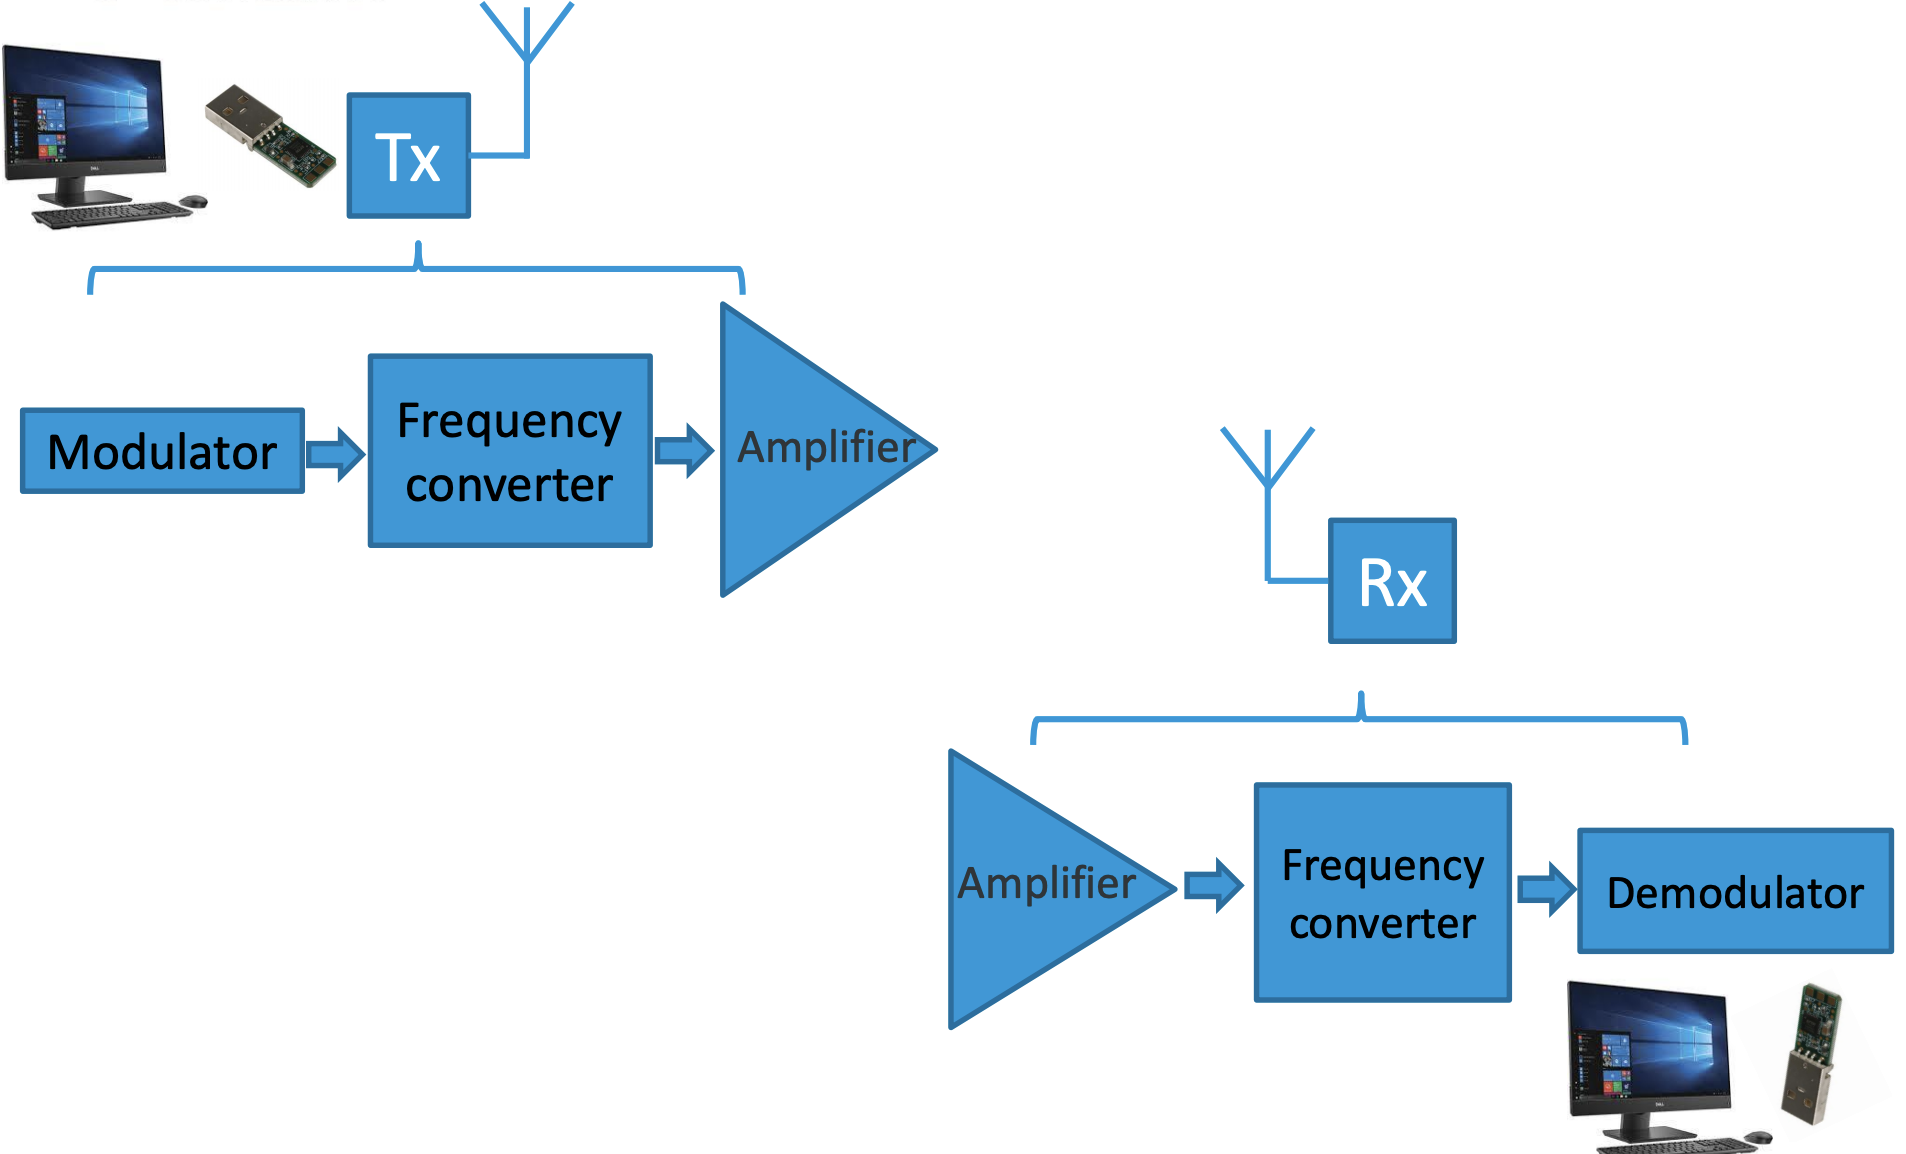
\includegraphics[scale=1]{system_structure}}
    \caption{The structure of a communication system}
    \label{fig:system_structure}
\end{figure}

\section{Operating frequencies}
For the choice of the frequency band, 2400Mhz-2500Mhz is chosen according to ISM: Frequency bands designated for Industrial, Scientific and Medical use.
The reason has been summarized in \hyperref[table:ofea]{Table \ref*{table:ofea}}.

\begin{table}[ht]
    \centering
    \begin{tabulary}{\linewidth}{|L |L| L|}
        \hline
        Frequency band & Standard & Estimation \\ 
        \hline
        433.05 - 434.79 MHz & 5.138 applies. Radiocommunication services must accept harmful interference from ISM. & Antenna size a bit impractical \\
        \hline
        2400 - 2500 MHz & 5.150 applies. Radiocommunication services must accept harmful interference from ISM & Available \\
        \hline
        5725 - 5785 MHz & 5.150 applies. Radiocommunication services must accept harmful interference from ISM. & Elevated cost \\
        \hline
        24.0 - 24.5 GHz & 5.150 applies. Radiocommunication services must accept harmful interference from ISM & Elevated cost and more challenging \\
        \hline
    \end{tabulary}
    \caption{Operating frequencies and estimation of availability}
    \label{table:ofea}
\end{table}

\section{Link budget}
The link budget of a transmitter and a receiver is:
\begin{equation}
    Link \, Budget = L_{FS}(dB) + G_{Tx}(dBi) + G_{Rx}(dBi)
\end{equation}

The term $L_{FS}$ is the free space loss:
\begin{equation}
    L_{FS}(dB) = 32.44 + 20\log{10}{(f(GHz))} + 20\log{10}{(d(meters))}
\end{equation}

Presuming the distance is in the range: $10cm - 2m$, $f = 2.45GHz$, then $L_{FS}$ is in the range $20.2dB - 30.7dB$.
Assuming the gain of the transmitter and the receiver are both $-6dBi$, then the link budget is in the range: $8.2dB - 18.7dB$.
For the requirements that the transmitter and the receiver should be $0dBm$,
\begin{equation}
    P_t(dBm) + G_t(dB) - Link \, Budget + G_r(dB) = P_r(dBm)
\end{equation}
is now re-arranged to: $G_t(dB) + G_r(dB) = Link \, Budget$. Assuming each gain stage is $20dB$, then one stage of amplifier at either transmitter or receiver should be enough.

\chapter{Patch antenna design}
The goal of this section is to design and optimize a quarter-wave matched micro-strip patch antenna fabricated on a FR4 substrate (Er = 4.3, tan(d) = 0.019, thickness = 1.6mm) at about 2.45 GHz.

\section{Concepts}
The principle of design a patched antenna is to achieve a $\lambda / 2$ resonator, as it is illustrated in \hyperref[fig:patch_principle]{Figure \ref*{fig:patch_principle}} that the reflection coefficient is 1 at the open circuit side, and it is approximately 1 on the other side with a thin linked signal feeder.

\begin{figure}[ht]
    \centerline{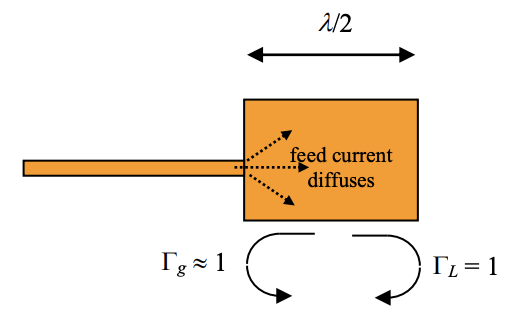
\includegraphics[scale=1.3]{patch_principle}}
    \caption{half-wavelength patch antenna}
    \label{fig:patch_principle}
\end{figure}

Therefore, it is necessary to have the length of the patch equal to $\lambda / 2$. However,  the electric fields are able to extend beyond
the physical edges of the patch as they curl downwards toward the ground plane. This effect called \emph{fringing}, and the result is that the patch appears to be electrically longer than its actual
physical length. Because of this, the required length of the patch, L, is given approximately by
the following equation:
\begin{equation}
    L = \frac{0.49 \lambda_0}{\sqrt{\epsilon_r}}
    \label{equ:patch_L}
\end{equation}
where $\epsilon_r$ is the dielectric constant of the substrate, and $\lambda_0$ is the wavelength in free space.

The top view of the patch antenna is shown in \hyperref[fig:top_view]{Figure \ref*{fig:top_view}}, which contains a $50 \Omega$ feed line, a quarter wave transformer, and the square patch with pre-calculated size.

\begin{figure}[ht]
    \centerline{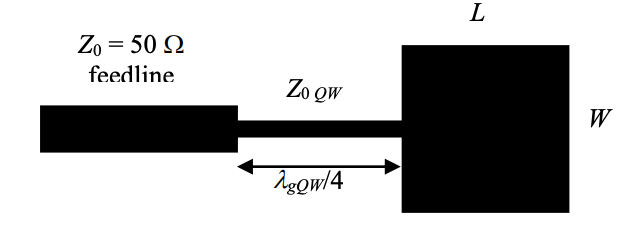
\includegraphics[scale=1.4]{top_view}}
    \caption{The top view of the patch antenna}
    \label{fig:top_view}
\end{figure}

The reason to add the quarter wave transformer is that the input impedance of the patch is very high. The impedance can be represented as \cite{input_impedance}:
\begin{equation}
    R_{IN} \approx 90 \bigg(\frac{\epsilon_r^2}{\epsilon_r - 1}\bigg) \bigg(\frac{L}{W} \bigg)^2
    \label{equ:patch_resistance}
\end{equation}

After calculating the value of $R_{IN}$, the impedance of the quarter wave transformer can be calculated from:

\begin{equation}
    Z_{0QW} = \sqrt{50R_{IN}}
    \label{equ:z0qw}
\end{equation}

\vspace{0.2cm}

The characteristic impedance of a transmission line obeys a complicated function of the line width $W$, the substrate height $h$, and the effective dielectric constant $\epsilon_{eff}$ \footnote{The equation of $\epsilon_{eff}$:\begin{equation}
    \epsilon_{eff} = \frac{\epsilon_r + 1}{2} + \frac{\epsilon_r - 1}{2} \bigg(\frac{\ln \frac{\pi}{2} + \frac{1}{\epsilon_r} \ln \frac{4}{\pi}}{\ln \frac{8h}{W}}\bigg)
    \label{equ:epsilon_eff}
\end{equation}}. For a given characteristic impedance $Z_0$, the required width of the transmission line is given by:

\begin{equation}
    W = \begin{cases}
        \frac{8h e^A}{e^{2A} - 2} &\text{valid when } W < 2h \\
        \frac{2h}{\pi}[B - 1 - \ln(2B - 1) + \frac{\epsilon_r - 1}{2 \epsilon_r} \{\ln(B - 1) + 0.39 - \frac{0.61}{\epsilon_r}\}] &\text{valid when } W > 2h
    \end{cases}
    \label{equ:w_calc}
\end{equation}

\vspace{0.2cm}

where

\begin{equation}
    A = \frac{Z_0}{60} \sqrt{\frac{\epsilon_r + 1}{2}} + \frac{\epsilon_r - 1}{\epsilon_r + 1}\bigg(0.23 + \frac{0.11}{\epsilon_r}\bigg)
    \label{equ:A}
\end{equation}
and

\begin{equation}
    B = \frac{377 \pi}{2 Z_0 \sqrt{\epsilon_r}}
    \label{equ:B}
\end{equation}

\section{Pre-lab tasks}
\begin{itemize}
    \item[1.] Calculate the required length $L$, width $W$, and the input resistance $R_{in}$ of a $2.5 \, GHz$ square patch antenna fabricated on FR4. \\
    From \hyperref[equ:patch_L]{Equation \ref*{equ:patch_L}}, L can be calculated from: $$L = \frac{0.49c}{\sqrt{\epsilon_r}f_0} = \frac{0.49 \cdot 3 \cdot 10^8}{\sqrt{4.3} \cdot 2.45 \cdot 10^9} = 2.89 \, cm,$$ where $c$ is the velocity of light, $f_0$ is the frequency: $2.45 GHz$.
    As it is a square patch, $W = L = 2.98 \, cm$. $R_{IN}$ can be calculated from \hyperref[equ:patch_resistance]{Equation \ref*{equ:patch_resistance}}: $$R_{IN} \approx 90 \bigg(\frac{4.3^2}{4.3 - 1}\bigg) = 504 \Omega$$
    \item[2.] Calculate the required characteristic impedance of the quarter wave transformer $Z_{0QW}$, its required width, its effective dielectric constant, its guided wavelength, and finally, its required length. \\
    From \hyperref[equ:z0qw]{Equation \ref*{equ:z0qw}}, $Z_{0QW} = \sqrt{50 \cdot 504} = 159 \Omega$. To calculate the width, use the first case of \hyperref[equ:w_calc]{Equation \ref*{equ:w_calc}}: $$A = \frac{159}{60} \sqrt{\frac{4.3 + 1}{2}} + \frac{4.3 - 1}{4.3 + 1} \bigg(0.23 + \frac{0.11}{4.3}\bigg) = 4.47,$$ $$W = \frac{8 \cdot 1.6 * e^{4.47}}{e^{2 \cdot 4.47 - 2}} = 1.08 mm$$
    The effective dielectric $\epsilon_{eff}$ can be calculated from \hyperref[equ:epsilon_eff]{Equation \ref*{equ:epsilon_eff}}: $$\epsilon_{eff} = \frac{4.3 + 1}{2} + \frac{4.3 - 1}{2} \bigg(\frac{\ln \frac{\pi}{2} + \frac{1}{4.3} \ln \frac{4}{\pi}}{\ln \frac{8 \cdot 1.6}{1.08}}\bigg) = 2.99$$
    To calculate the guided wavelength, first compute the phase velocity: $$v_{\phi} = \frac{1}{\sqrt{\mu\epsilon}} = \frac{c}{\sqrt{\mu_r \epsilon_r}} = \frac{3 \cdot 10^8}{\sqrt{2.99}} = 1.73 \cdot 10^8 \enspace m/s$$
    Then, $$\lambda_g = \frac{v_\phi}{f} = \frac{1.73 \cdot 10^8}{2.45 \cdot 10^9} = 0.12 \enspace m$$
    Therefore, the quarter-wavelength transformer could have the length: $L = \frac{\lambda_g}{4} = 3 \enspace cm$.
    \item[3.] Calculate the required width and the guided wavelength of the $50 \Omega$ feed line. \\
    To calculate the width of the feed line, use the second case of \hyperref[equ:w_calc]{Equation \ref*{equ:w_calc}}:
    $$B = \frac{377\pi}{2 \cdot 50 \cdot \sqrt{4.3}} = 5.71,$$ $$W = \frac{2 \cdot 1.6}{\pi}[5.71 - 1 - \ln(2 \cdot 5.71 - 1) + \frac{4.3 - 1}{2 \cdot 4.3} \{\ln(5.71 - 1) + 0.39 - \frac{0.11}{4.3}\}] = 3.11 \enspace mm$$
    The guided wavelength is the same as that of task 2. $\lambda_g = 0.12 \enspace m$.
\end{itemize}

% \section{Design with ADS}
% This sections introduces the procedures of the designation of the patch antenna using \emph{Keysight ADS}.
% The goal is to design and optimize a quarter-wave matched micro-strip patch antenna fabricated on a FR4 substrate operating at about 2.5GHz. The impedance match of the antenna must be better than -20 dB at the design frequency.
\section{Design and performance test}
The design of the patch antenna is under the aid of \emph{Keysight ADS}. The parameters have been well tunned during the process of simulation in the laboratory. Thus, it was expected the produced antenna would behave the same as what had been shown on the simulation results.
This section shows the produced antennas and their characteristics.

\hyperref[fig:antenna_photo]{Figure \ref*{fig:antenna_photo}} shows the antenna finally made. The two antennas are both based on the same project schematic, thus the performance should be the same.

\begin{figure}[ht]
    \centerline{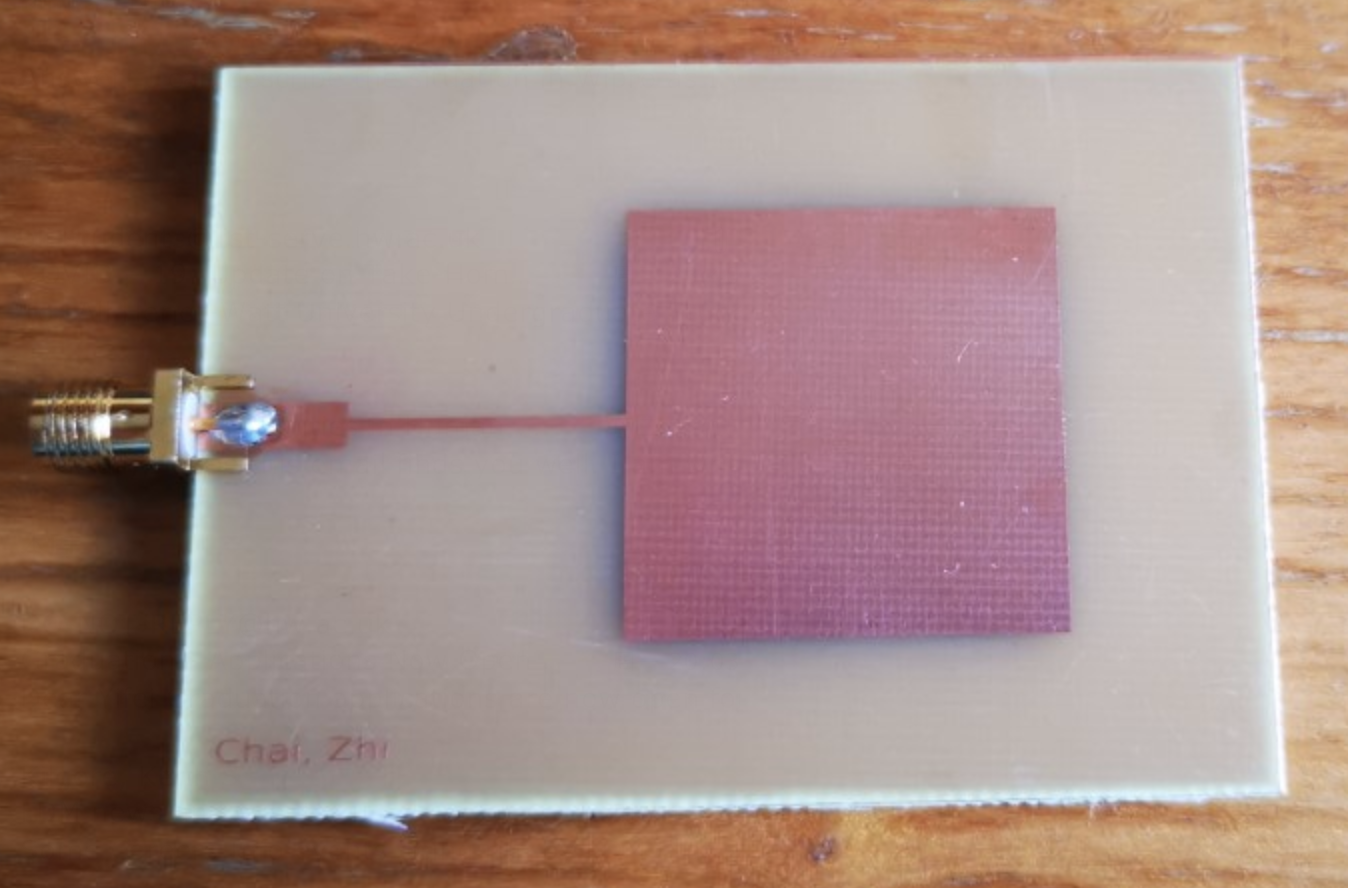
\includegraphics[scale=0.8]{antenna_photo}}
    \caption{Capture of successfully made antenna}
    \label{fig:antenna_photo}
\end{figure}

The performance of the antenna was tested through pocket VNA. Surprisingly, the performance of the two antennas are different, though they showed impedance match at around 2.45 GHz. \hyperref[fig:s11_antenna_1]{Figure \ref*{fig:s11_antenna_1}} and \hyperref[fig:s11_antenna_2]{Figure \ref*{fig:s11_antenna_2}} depict the $S_{11}$ property of the antennas. The match of impedance requires that the value of $S_{11}$ be smaller than -10 dB. Apparently, the two antennas have passed the this requirement. However, the second sample behaved much better.

\begin{figure}[ht]
    \centerline{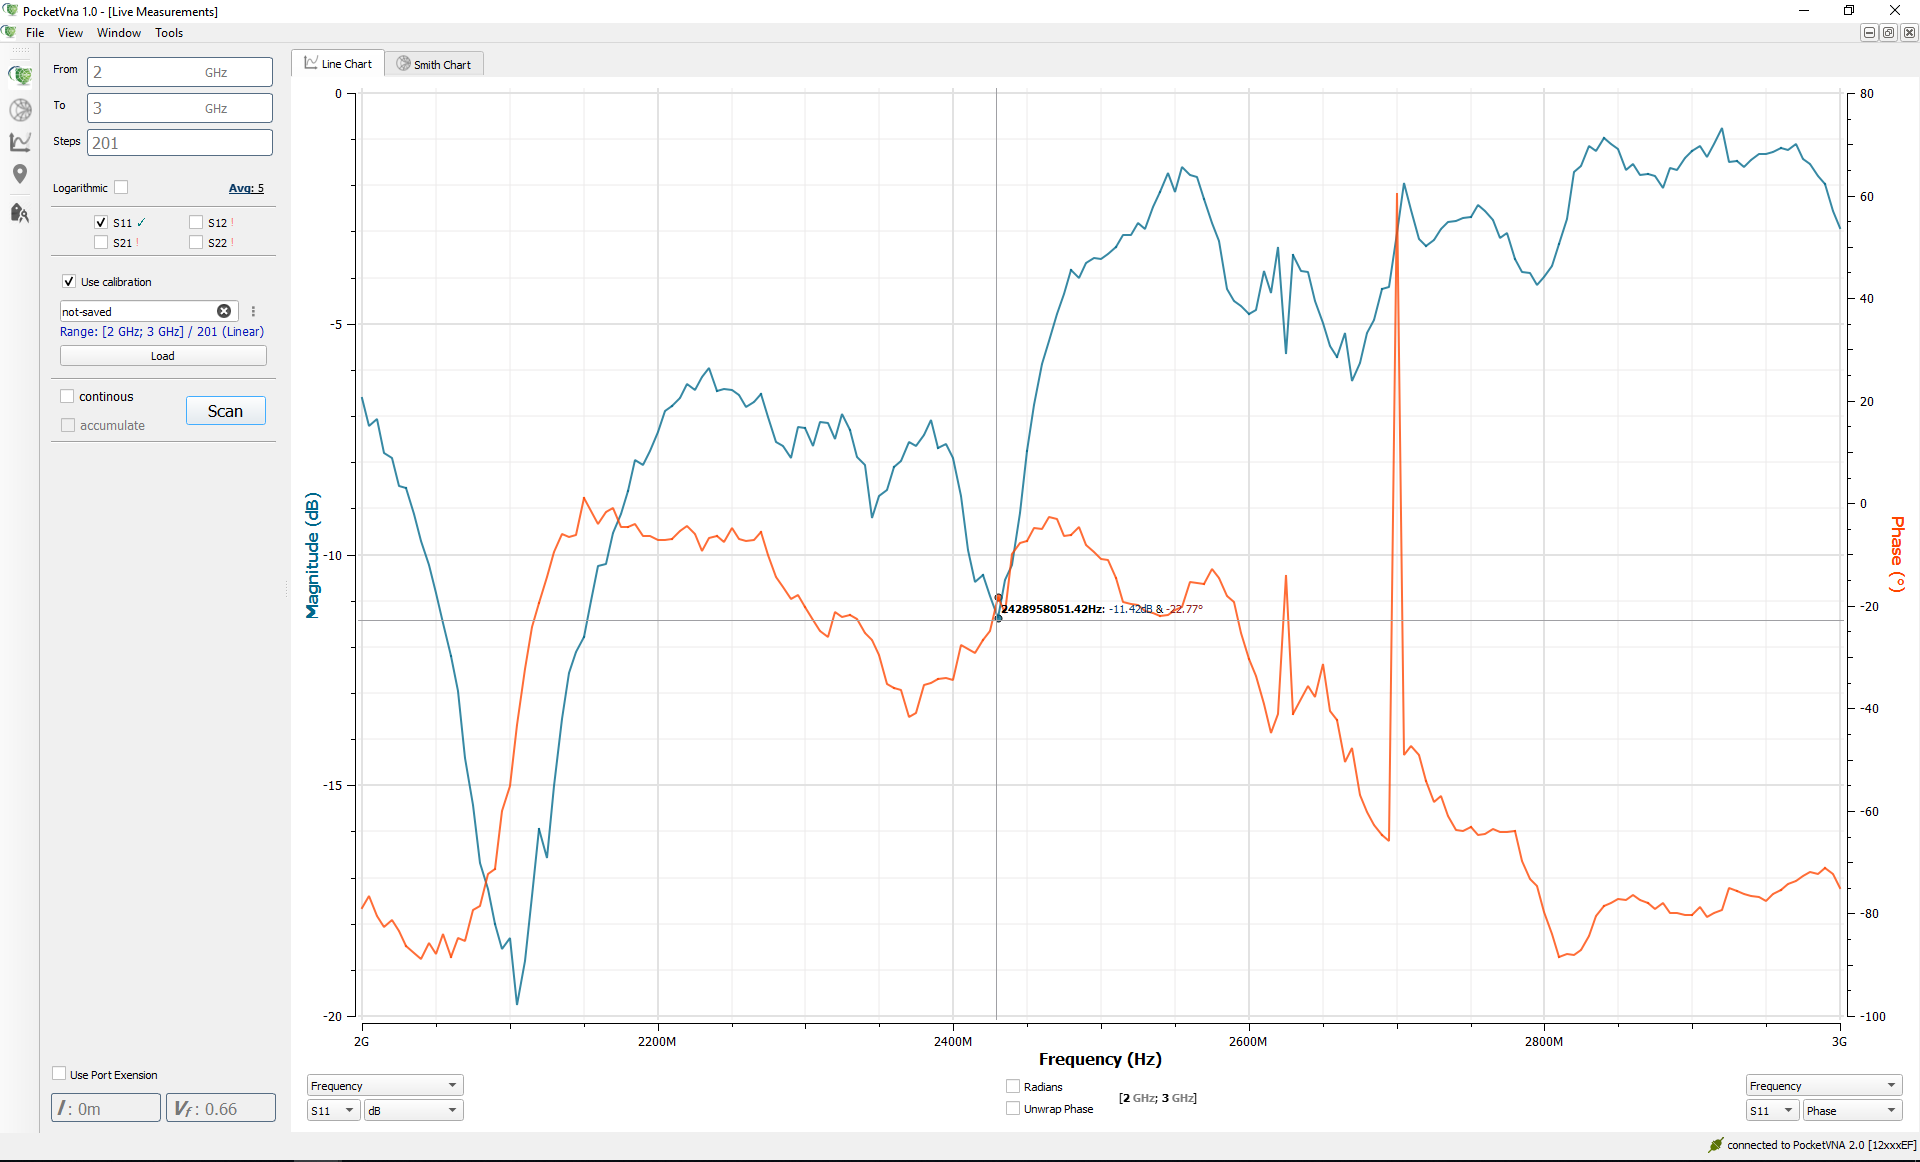
\includegraphics[scale=0.35]{s11_antenna_1}}
    \caption{$S_{11}$ of the first antenna}
    \label{fig:s11_antenna_1}
\end{figure}

\begin{figure}[ht]
    \centerline{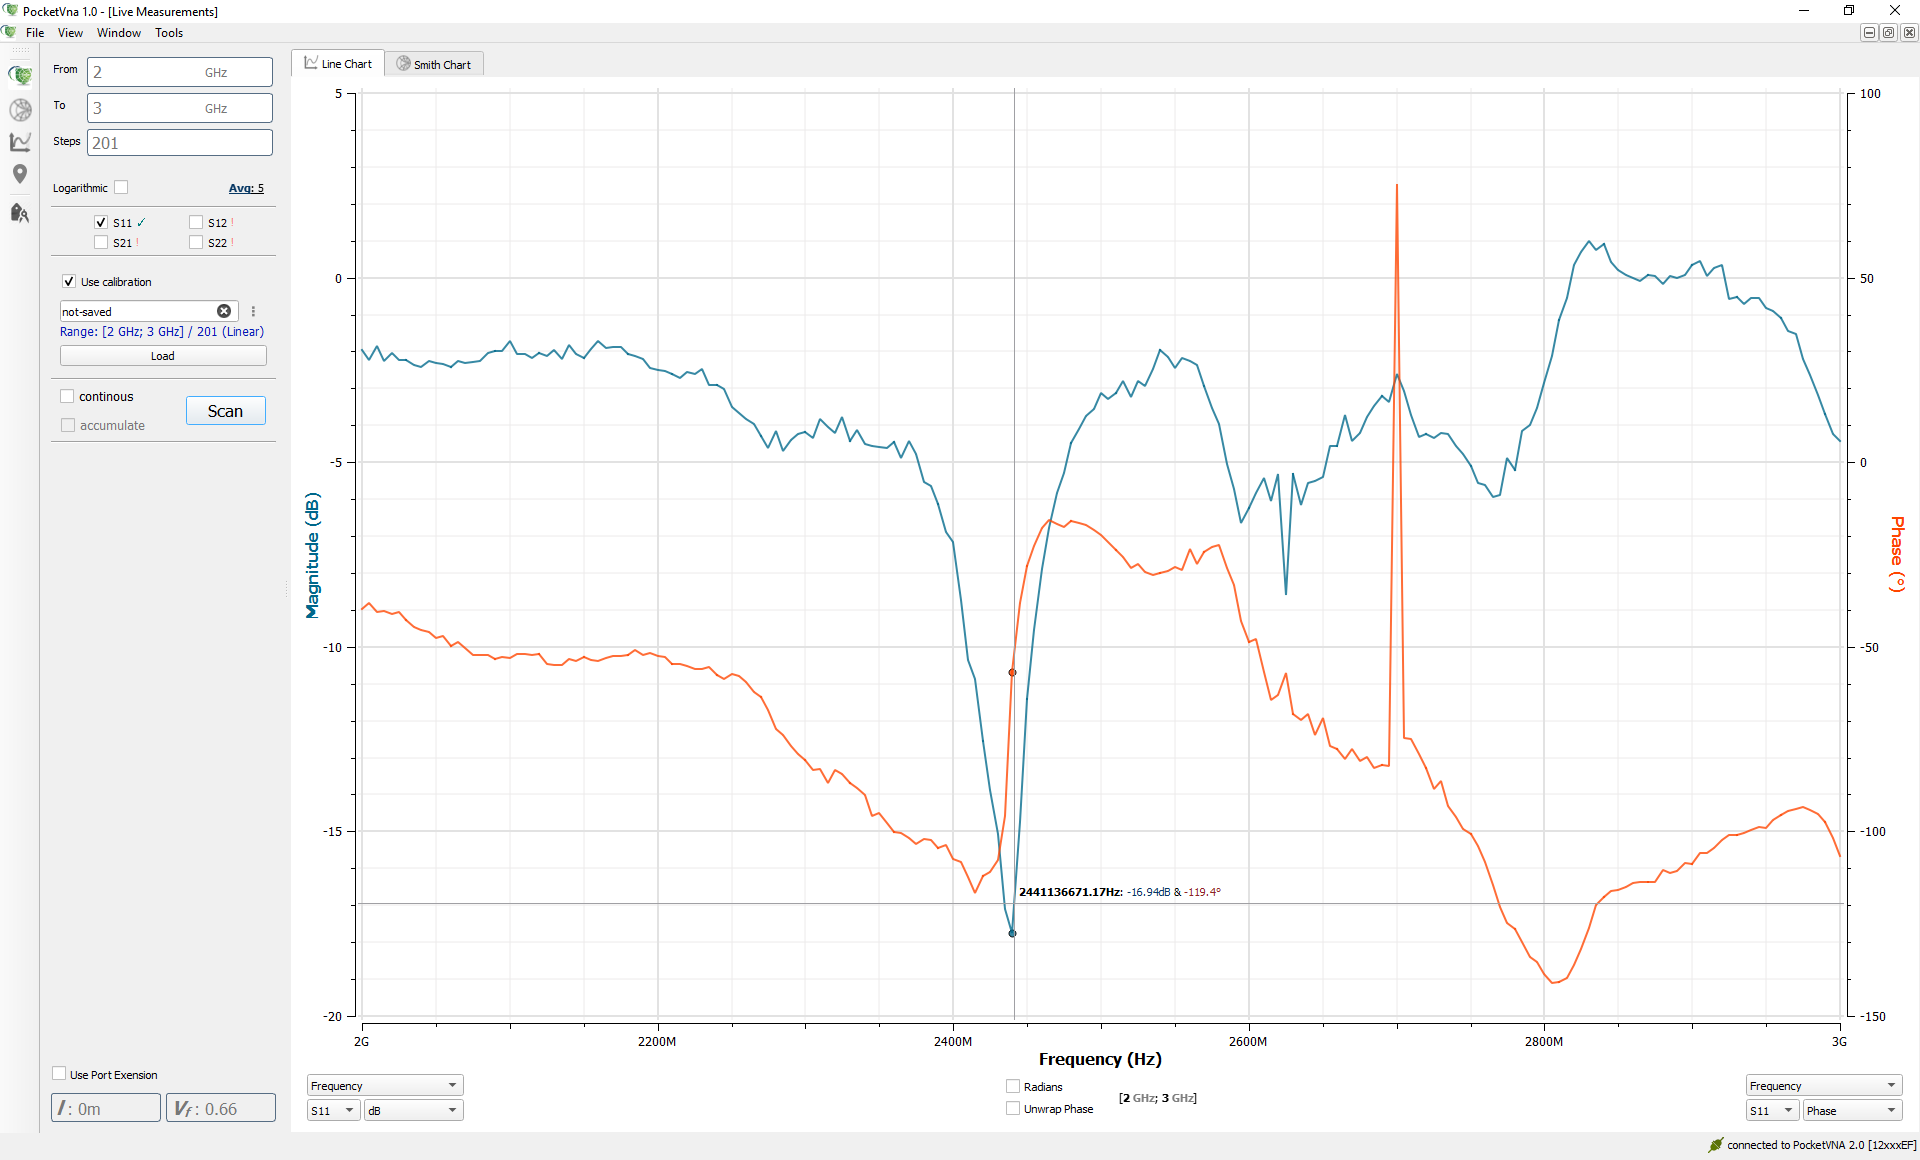
\includegraphics[scale=0.35]{s11_antenna_2}}
    \caption{$S_{11}$ of the second antenna}
    \label{fig:s11_antenna_2}
\end{figure}

\chapter{Amplifier design}
% Justify the MOSFET devices choice and describe sub-sequent unavailability of the device.
% You will be then showing only simulation results.
This section mainly describe the design of a low noise amplifier based on \textbf{ATF-58143}. 

The reason to choose this device is that:
\begin{itemize}
    \item[1.] It is available to buy: from \emph{farnell} or \emph{digikey}.
    \item[2.] It has a model than can be used in \emph{ADS}.
\end{itemize}

% To fill
The  DC-IV characterization schematic in ADS and results.

Show S parameters simulations over a wide frequency range for a given bias point, include
ADS schematic.

Show stability analysis before and after stabilization.

However, owing to some reasons, this device was no longer available at the time the laboratory was holding.
The new solution is to use a the Bipolar - RF transistor \textbf{BFU610}.\\
Here the simulation of \textbf{ATF-58143} will be given. The procedures of simulation will is given below.
\begin{itemize}
    \item Basic circuit construction of low noise amplifier
    \item Source-Load matching
    \item adding junctions and gaps
    \item output power test
\end{itemize}
\begin{figure}
    \centerline{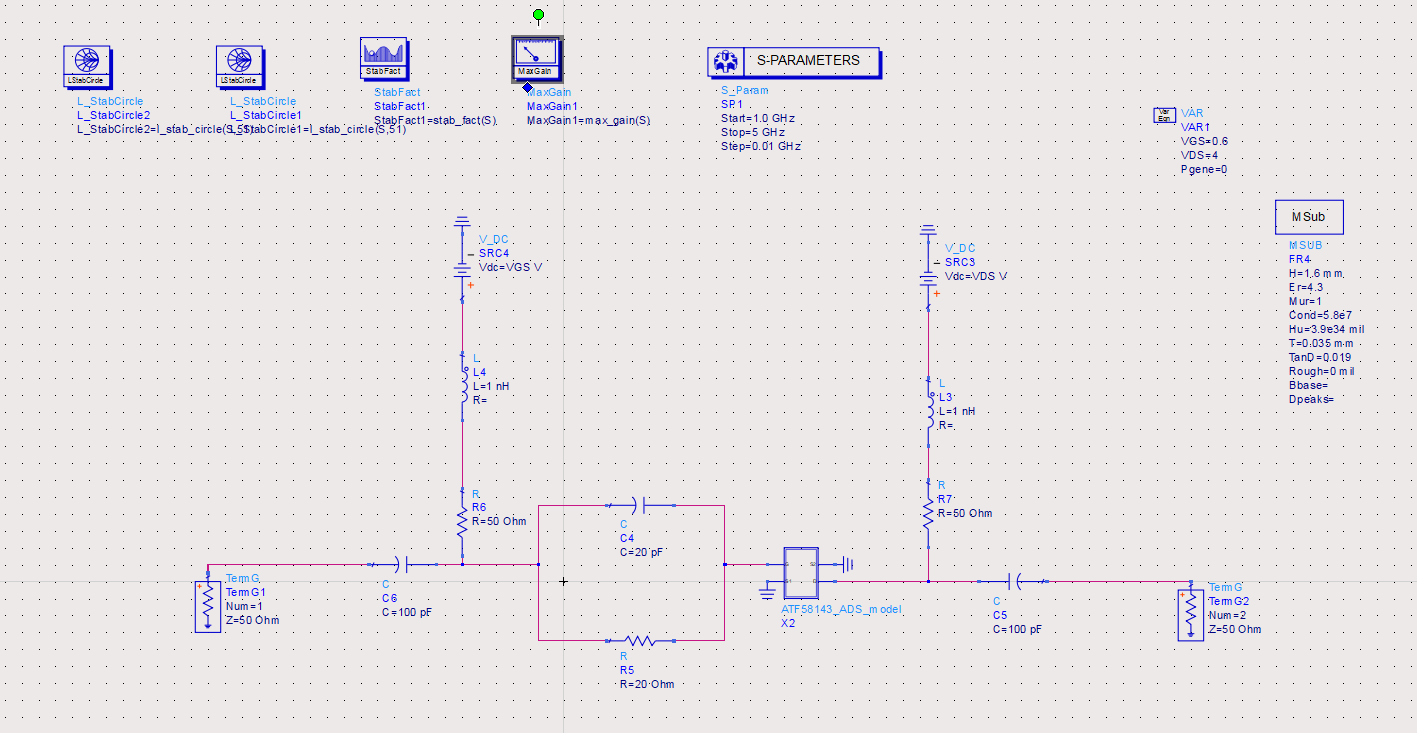
\includegraphics[scale=0.5]{LNABasicCicuit.PNG}}
    \caption{Basic structure of Low Noise Amplifier}
    \label{LNA}
\end{figure}
In \hyperref[LNA]{Figure \ref*{LNA}}, the capacitor, resistor and inductor separate DC and AC. Now the source and load is mismatch.
\begin{figure}
    \centerline{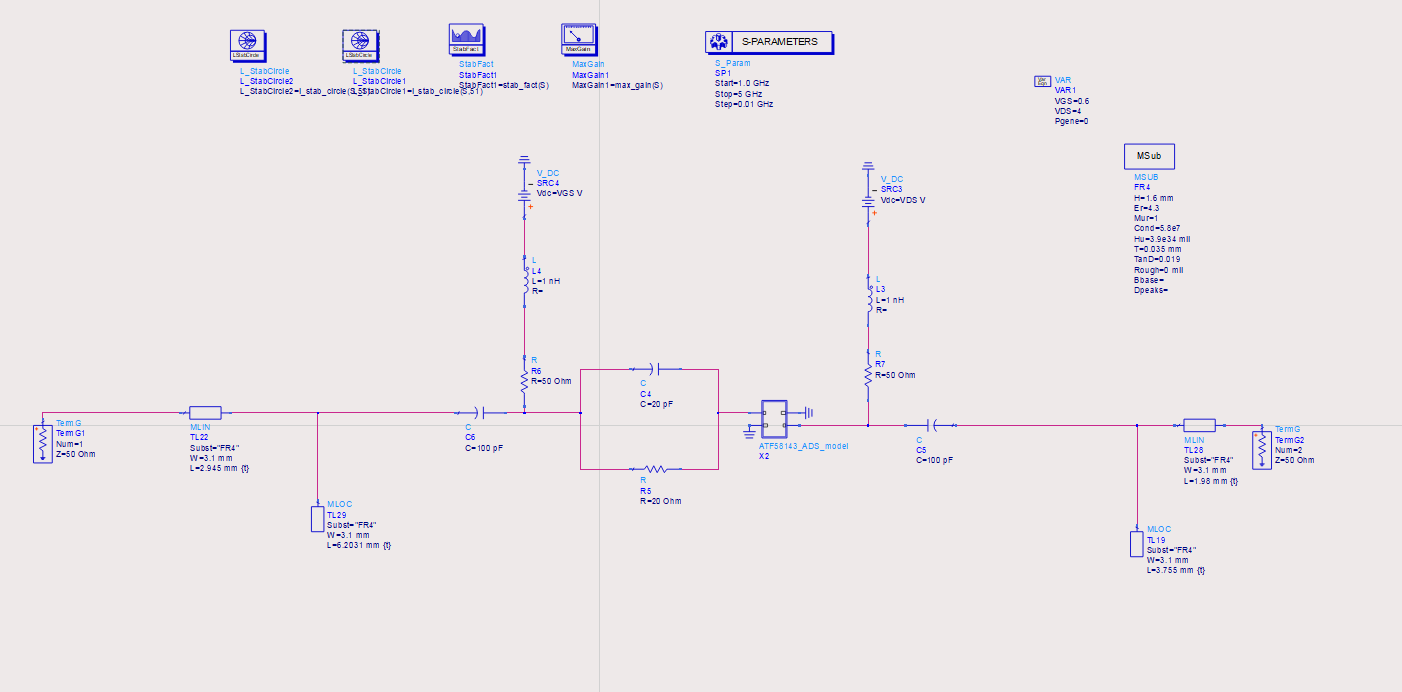
\includegraphics[scale=0.5]{FirstMatching.PNG}}
    \caption{Source Load Matching}
    \label{fm}
\end{figure}
\hyperref[fm]{Figure \ref*{fm}} shows the circuit after matching. $S_{21}$ is higher than the circuit without matching.\\
Junctions and gaps are needed since when printing the board, capacitors, inductors and resistors can not be printed on it. But the 
space should be given for them. Using gaps to simulate the spaces for those components. Using junctions to simulate the intersections.
\begin{figure}
    \centerline{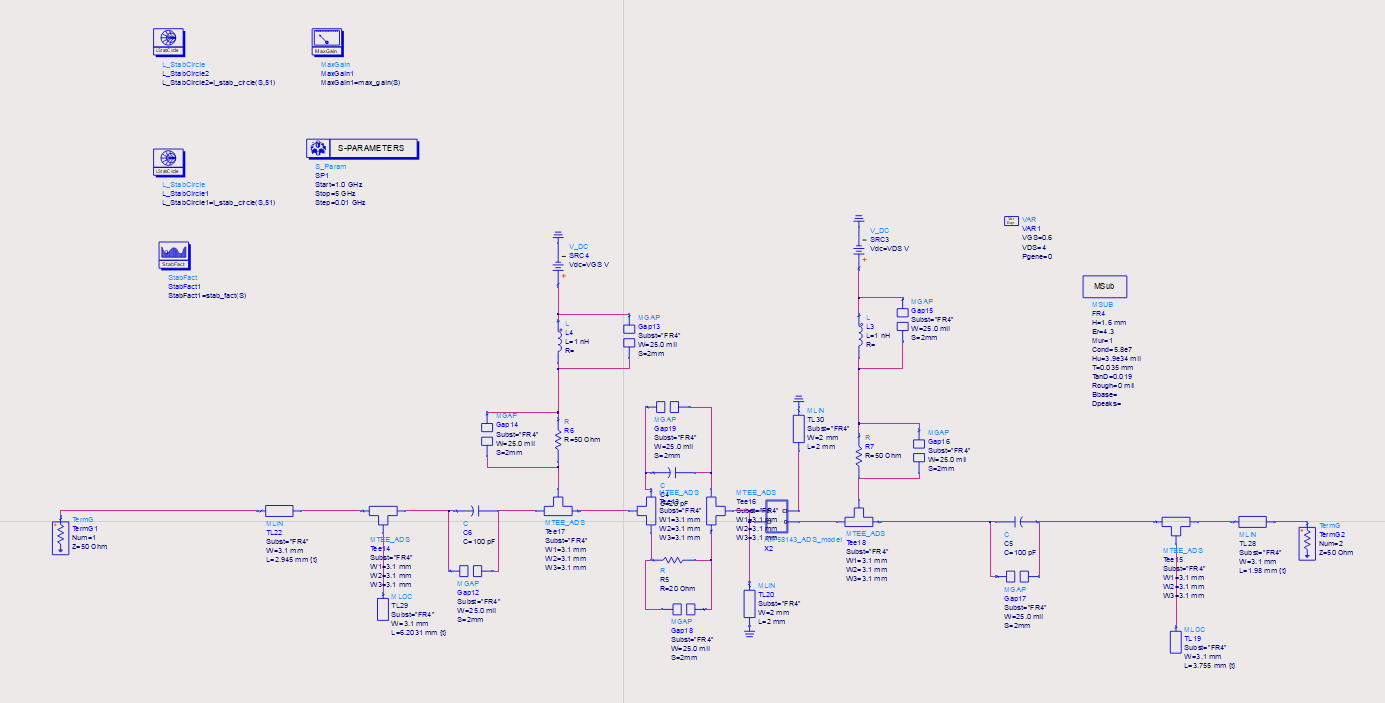
\includegraphics[scale=0.5]{Junctions_Added.PNG}}
    \caption{Circuit with T-Junctions and gaps}
    \label{junctions}
\end{figure}
\begin{figure}
    \centerline{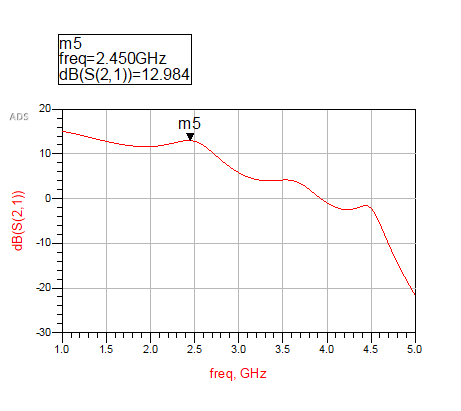
\includegraphics{Junctions_S21.PNG}}
    \caption{$S_{21}$ value}
    \label{S21}
\end{figure}
\hyperref[junctions]{Figure \ref*{junctions}} shows the circuit after adding T-junctions and gaps. \hyperref[S21]{Figure \ref*{S21}} shows the $S_{21}$ of this circuit. Output power test needs 
replace TermG with AC source and observe the $P_{in}$, $P_{out}$ relationship.
\begin{figure}
    \centerline{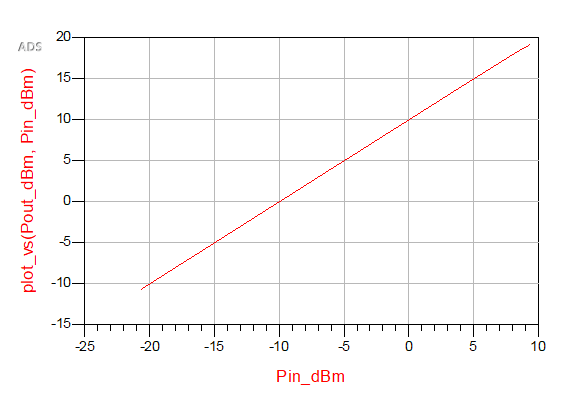
\includegraphics[]{P_inP_out.PNG}}
    \caption{$P_{in}$-$P_{out}$ relationship}
    \label{inout}
\end{figure}
\begin{figure}
    \centerline{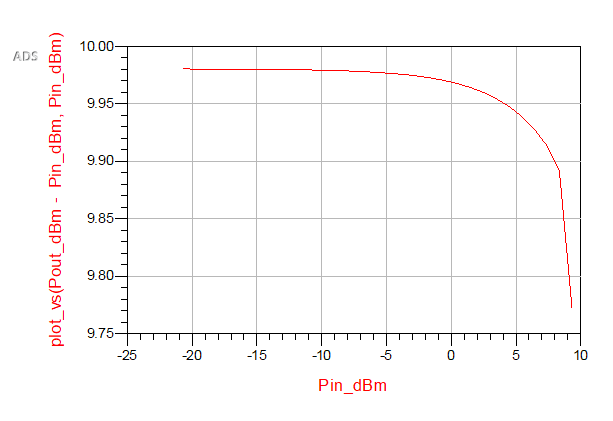
\includegraphics{P_inP_outSlope.PNG}}
    \caption{Linear region}
    \label{linearregion}
\end{figure}
\hyperref[inout]{Figure \ref*{inout}} shows the relationship between $P_{in}$ and $P_{out}$. From the graph, it satisfies the property of a linear amplifier. \hyperref[linearregion]{Figure \ref*{linearregion}} shows the 
linear amplification region of the low noise amplifier. Once beyond the linear region, output signal will have a distortion.
\chapter{Low Pass Filter}
In the receiver side. High frequency carrier needs to be filtered out. A low pass filter is applied at the receiver side. The circuit of low pass filter is given in \hyperref[fig:typical_detector_circuit]{Figure \ref*{fig:typical_detector_circuit}}.
\hyperref[LPFSimulationResult]{Figure \ref*{LPFSimulationResult}} shows the simulation results of the low pass filter. \hyperref[RealLPF]{Figure \ref*{RealLPF}} is the real low pass filter used in this wireless system. The difference between real
circuit and designed circuit is the real circuit does not contain capacitor. From \hyperref[fig:LPF2]{Figure \ref*{fig:LPF2}} to \hyperref[fig:LPF1K]{Figure \ref*{fig:LPF1K}} is the test result with 2Hz signal, 5Hz signal and 1KHz signal. Result is shown
on the oscilliscope.
% \begin{figure}[H]
%     \centerline{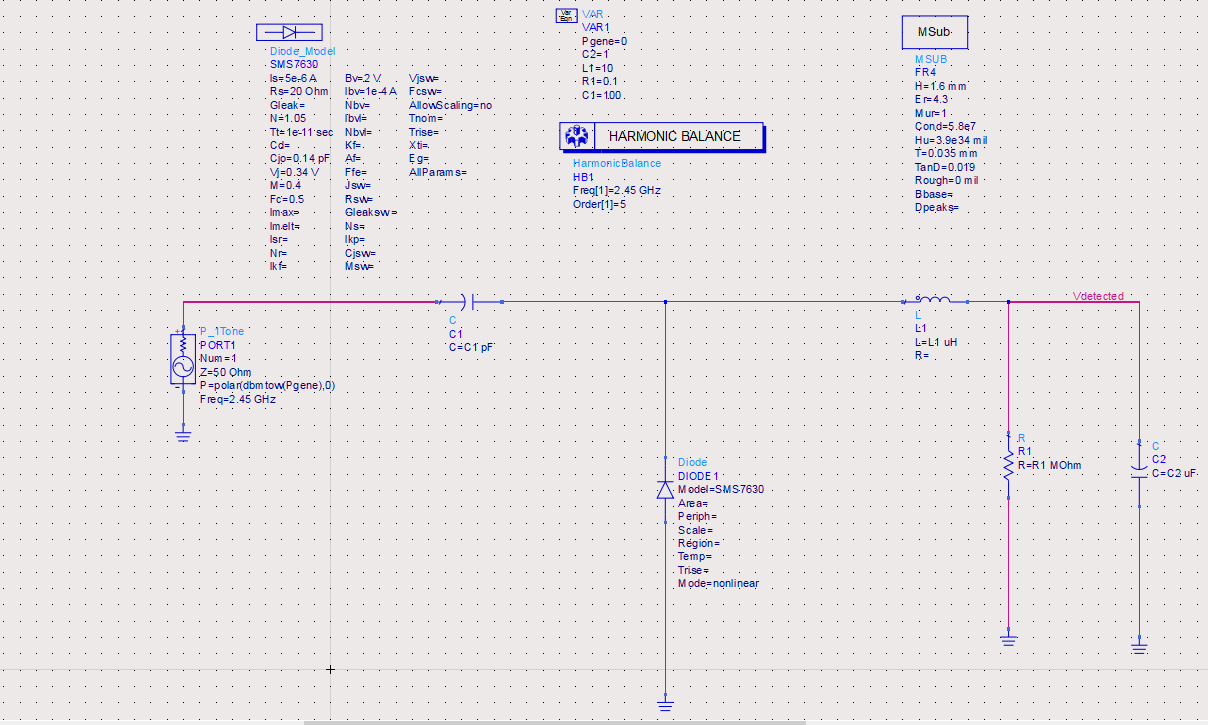
\includegraphics[scale=0.5]{LPF_circuit.PNG}}
%     \caption{Low pass filter circuit}
%     \label{LPF}
% \end{figure}
\begin{figure}[ht]
    \centerline{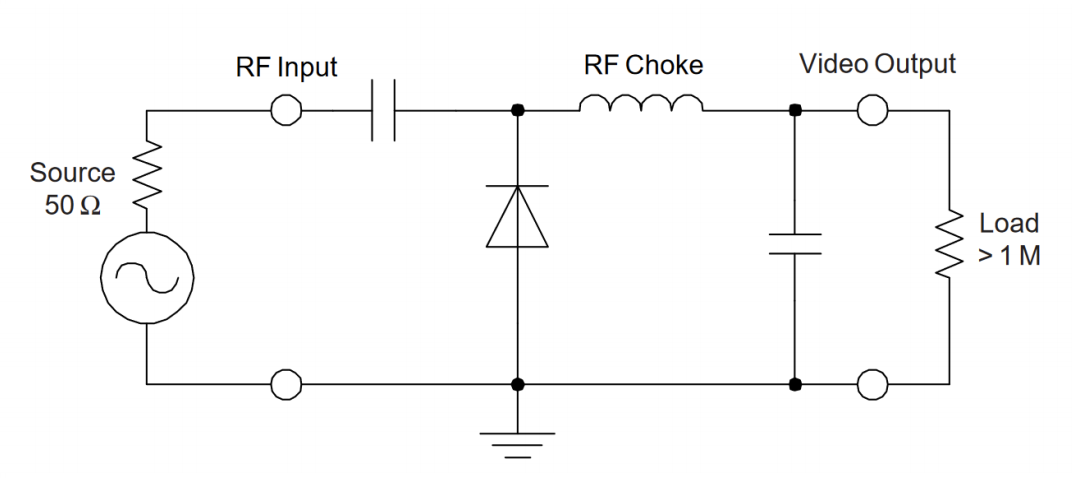
\includegraphics[scale=1]{typical_detector_circuit}}
    \caption{Circuit of a low pass filter}
    \label{fig:typical_detector_circuit}
\end{figure}

\begin{figure}[H]
    \centerline{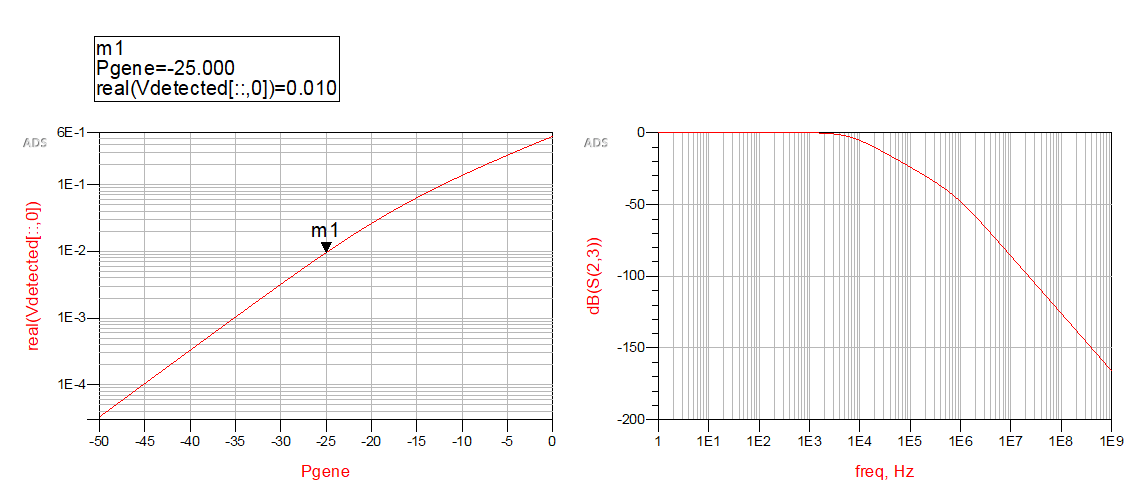
\includegraphics[scale=0.5]{LPF_SimulationResult.PNG}}
    \caption{Low pass filter simulation result}
    \label{LPFSimulationResult}
\end{figure}

\begin{figure}[H]
    \centerline{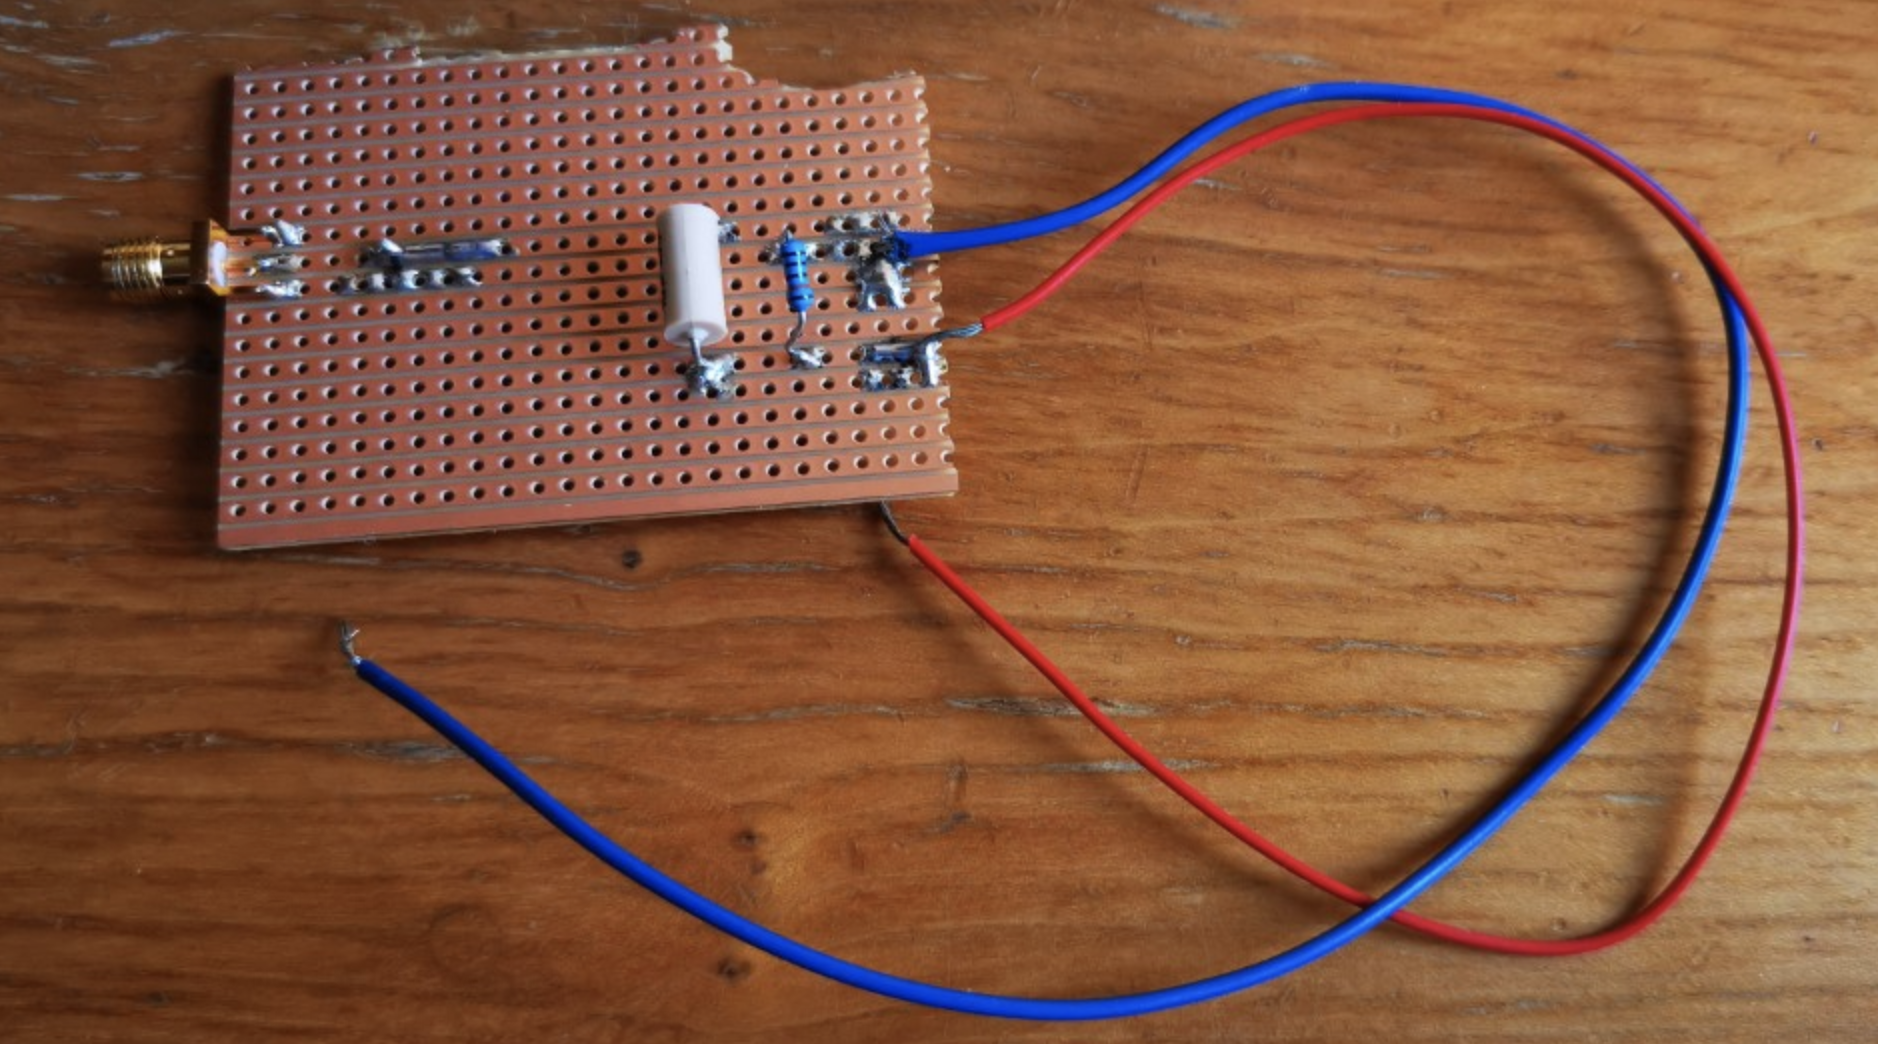
\includegraphics[scale=0.5]{rectifier.png}}
    \caption{Low pass filter(real circuit)}
    \label{RealLPF}
\end{figure}

\begin{figure}[H]
    \centerline{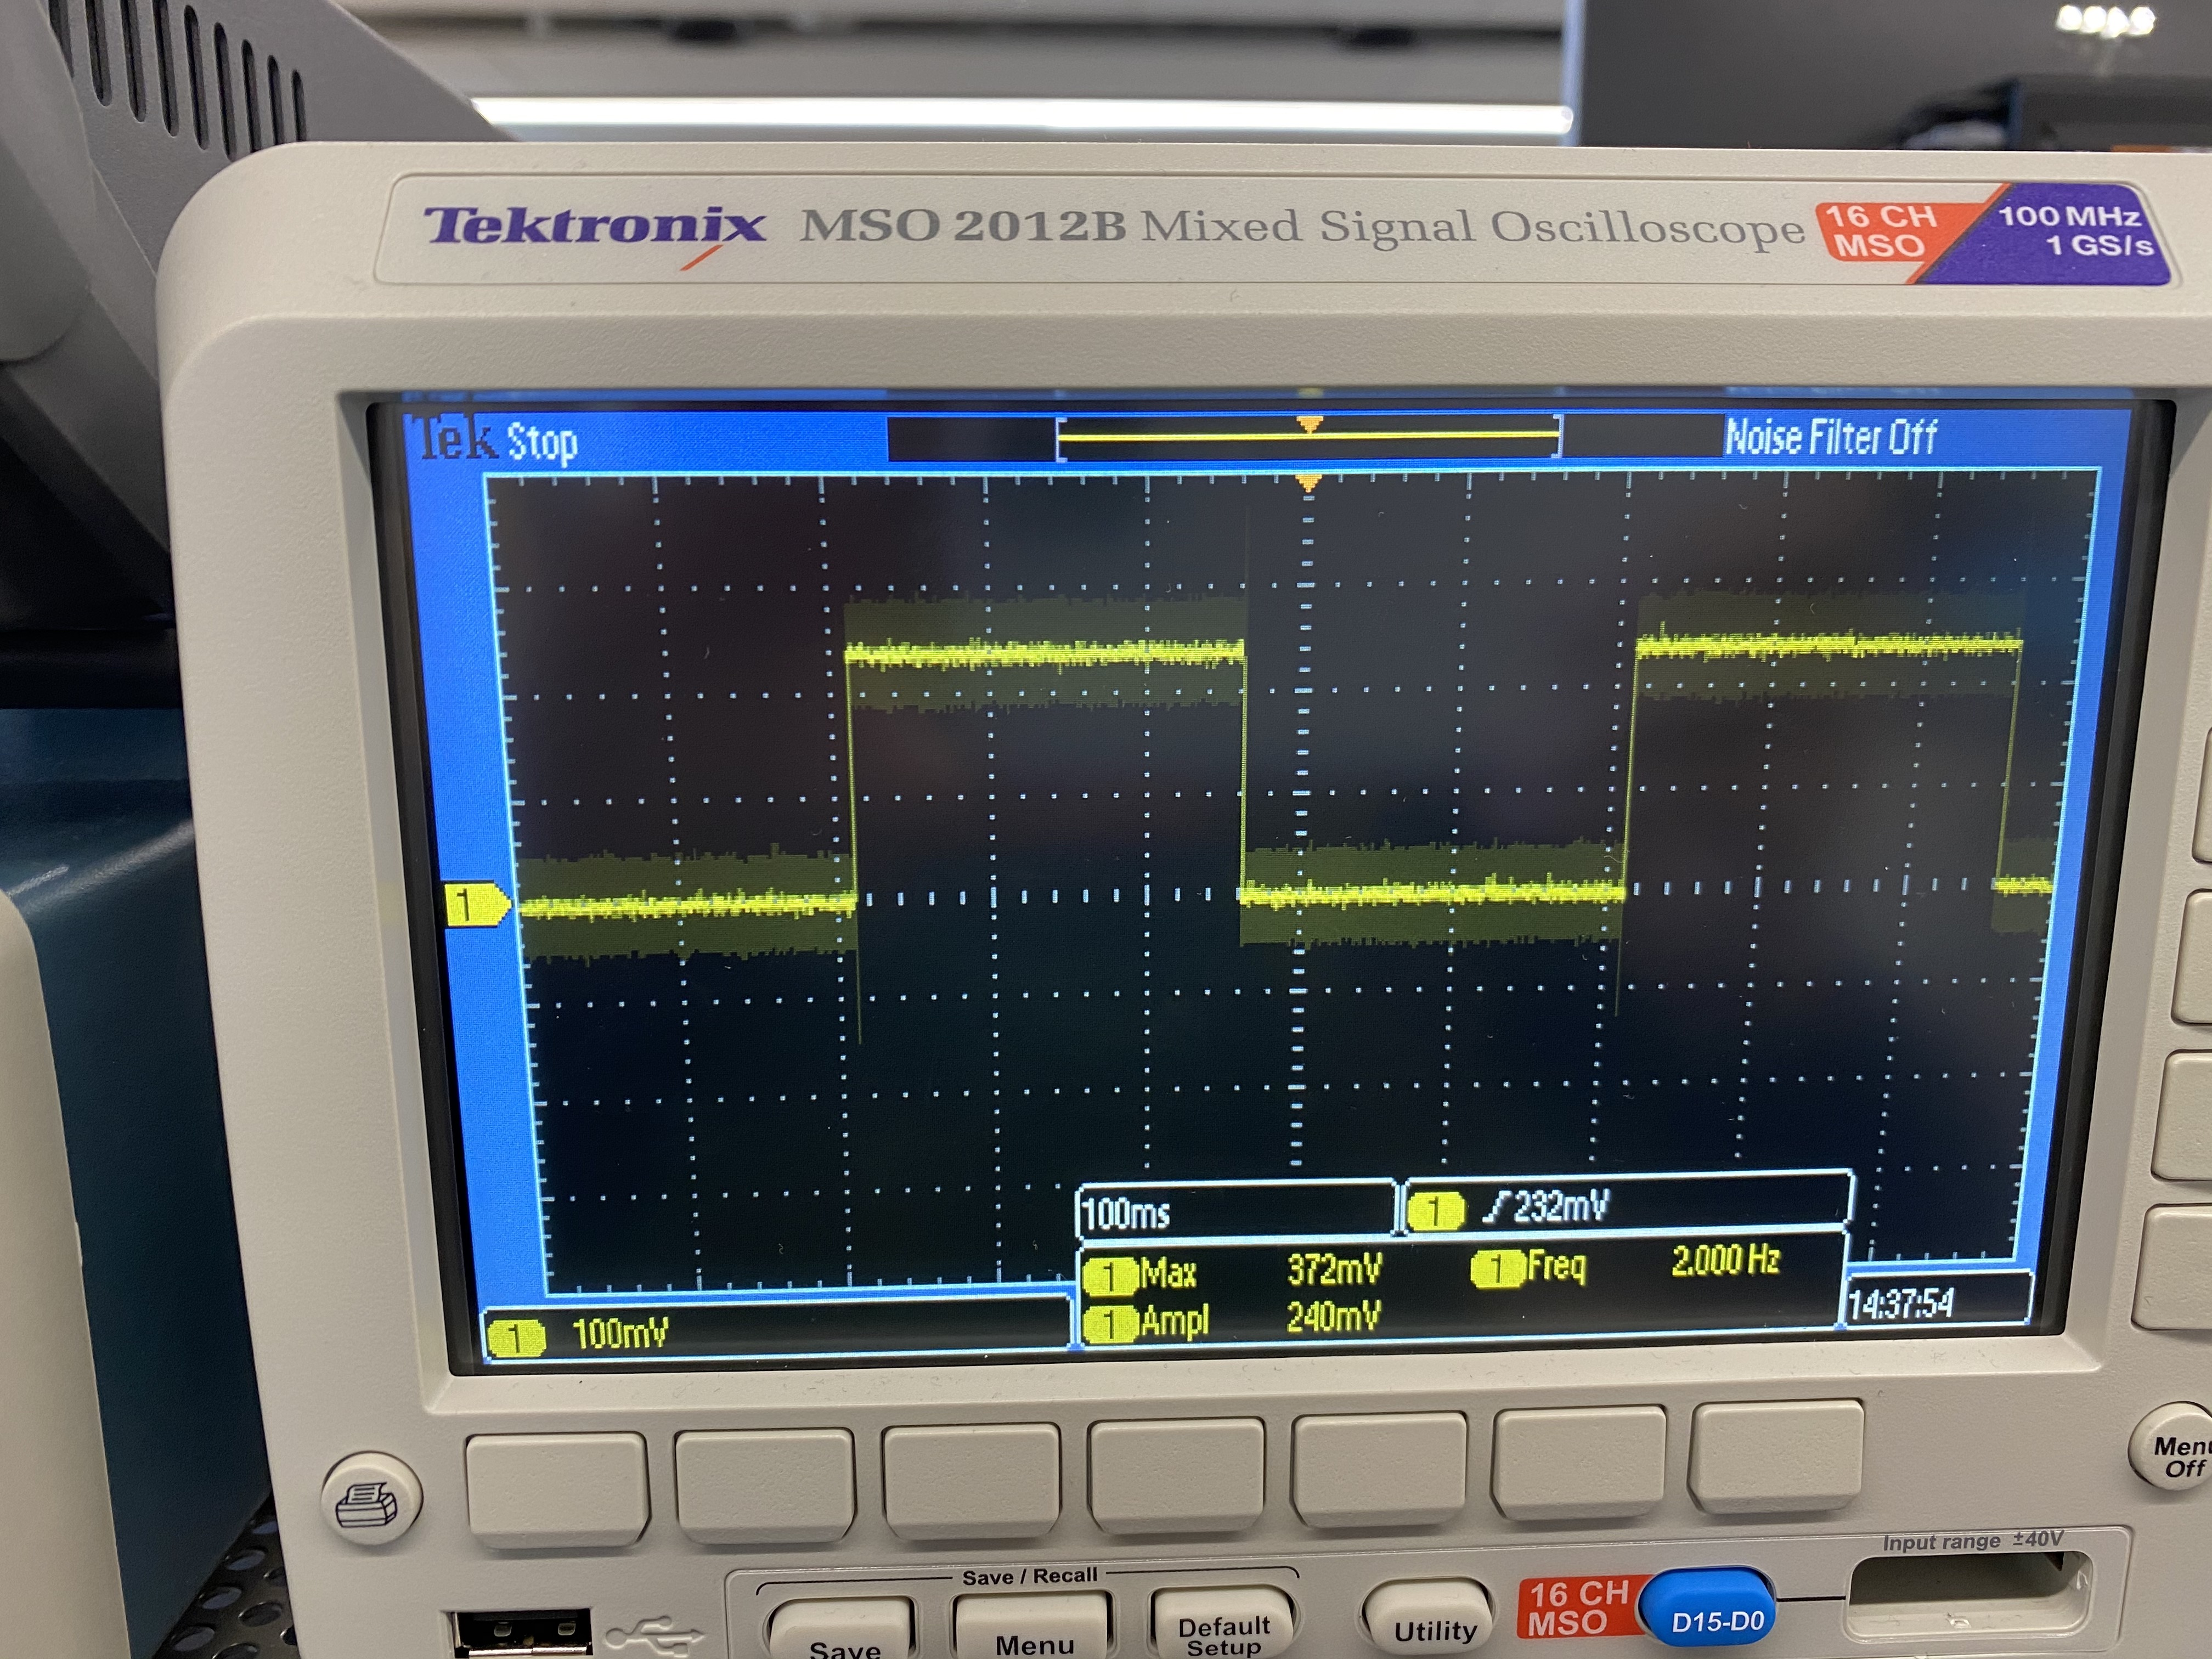
\includegraphics[scale=0.1]{LPFTest2Hz.PNG}}
    \caption{LPF test with 2Hz basband signal}
    \label{fig:LPF2}
\end{figure}

\begin{figure}[H]
    \centerline{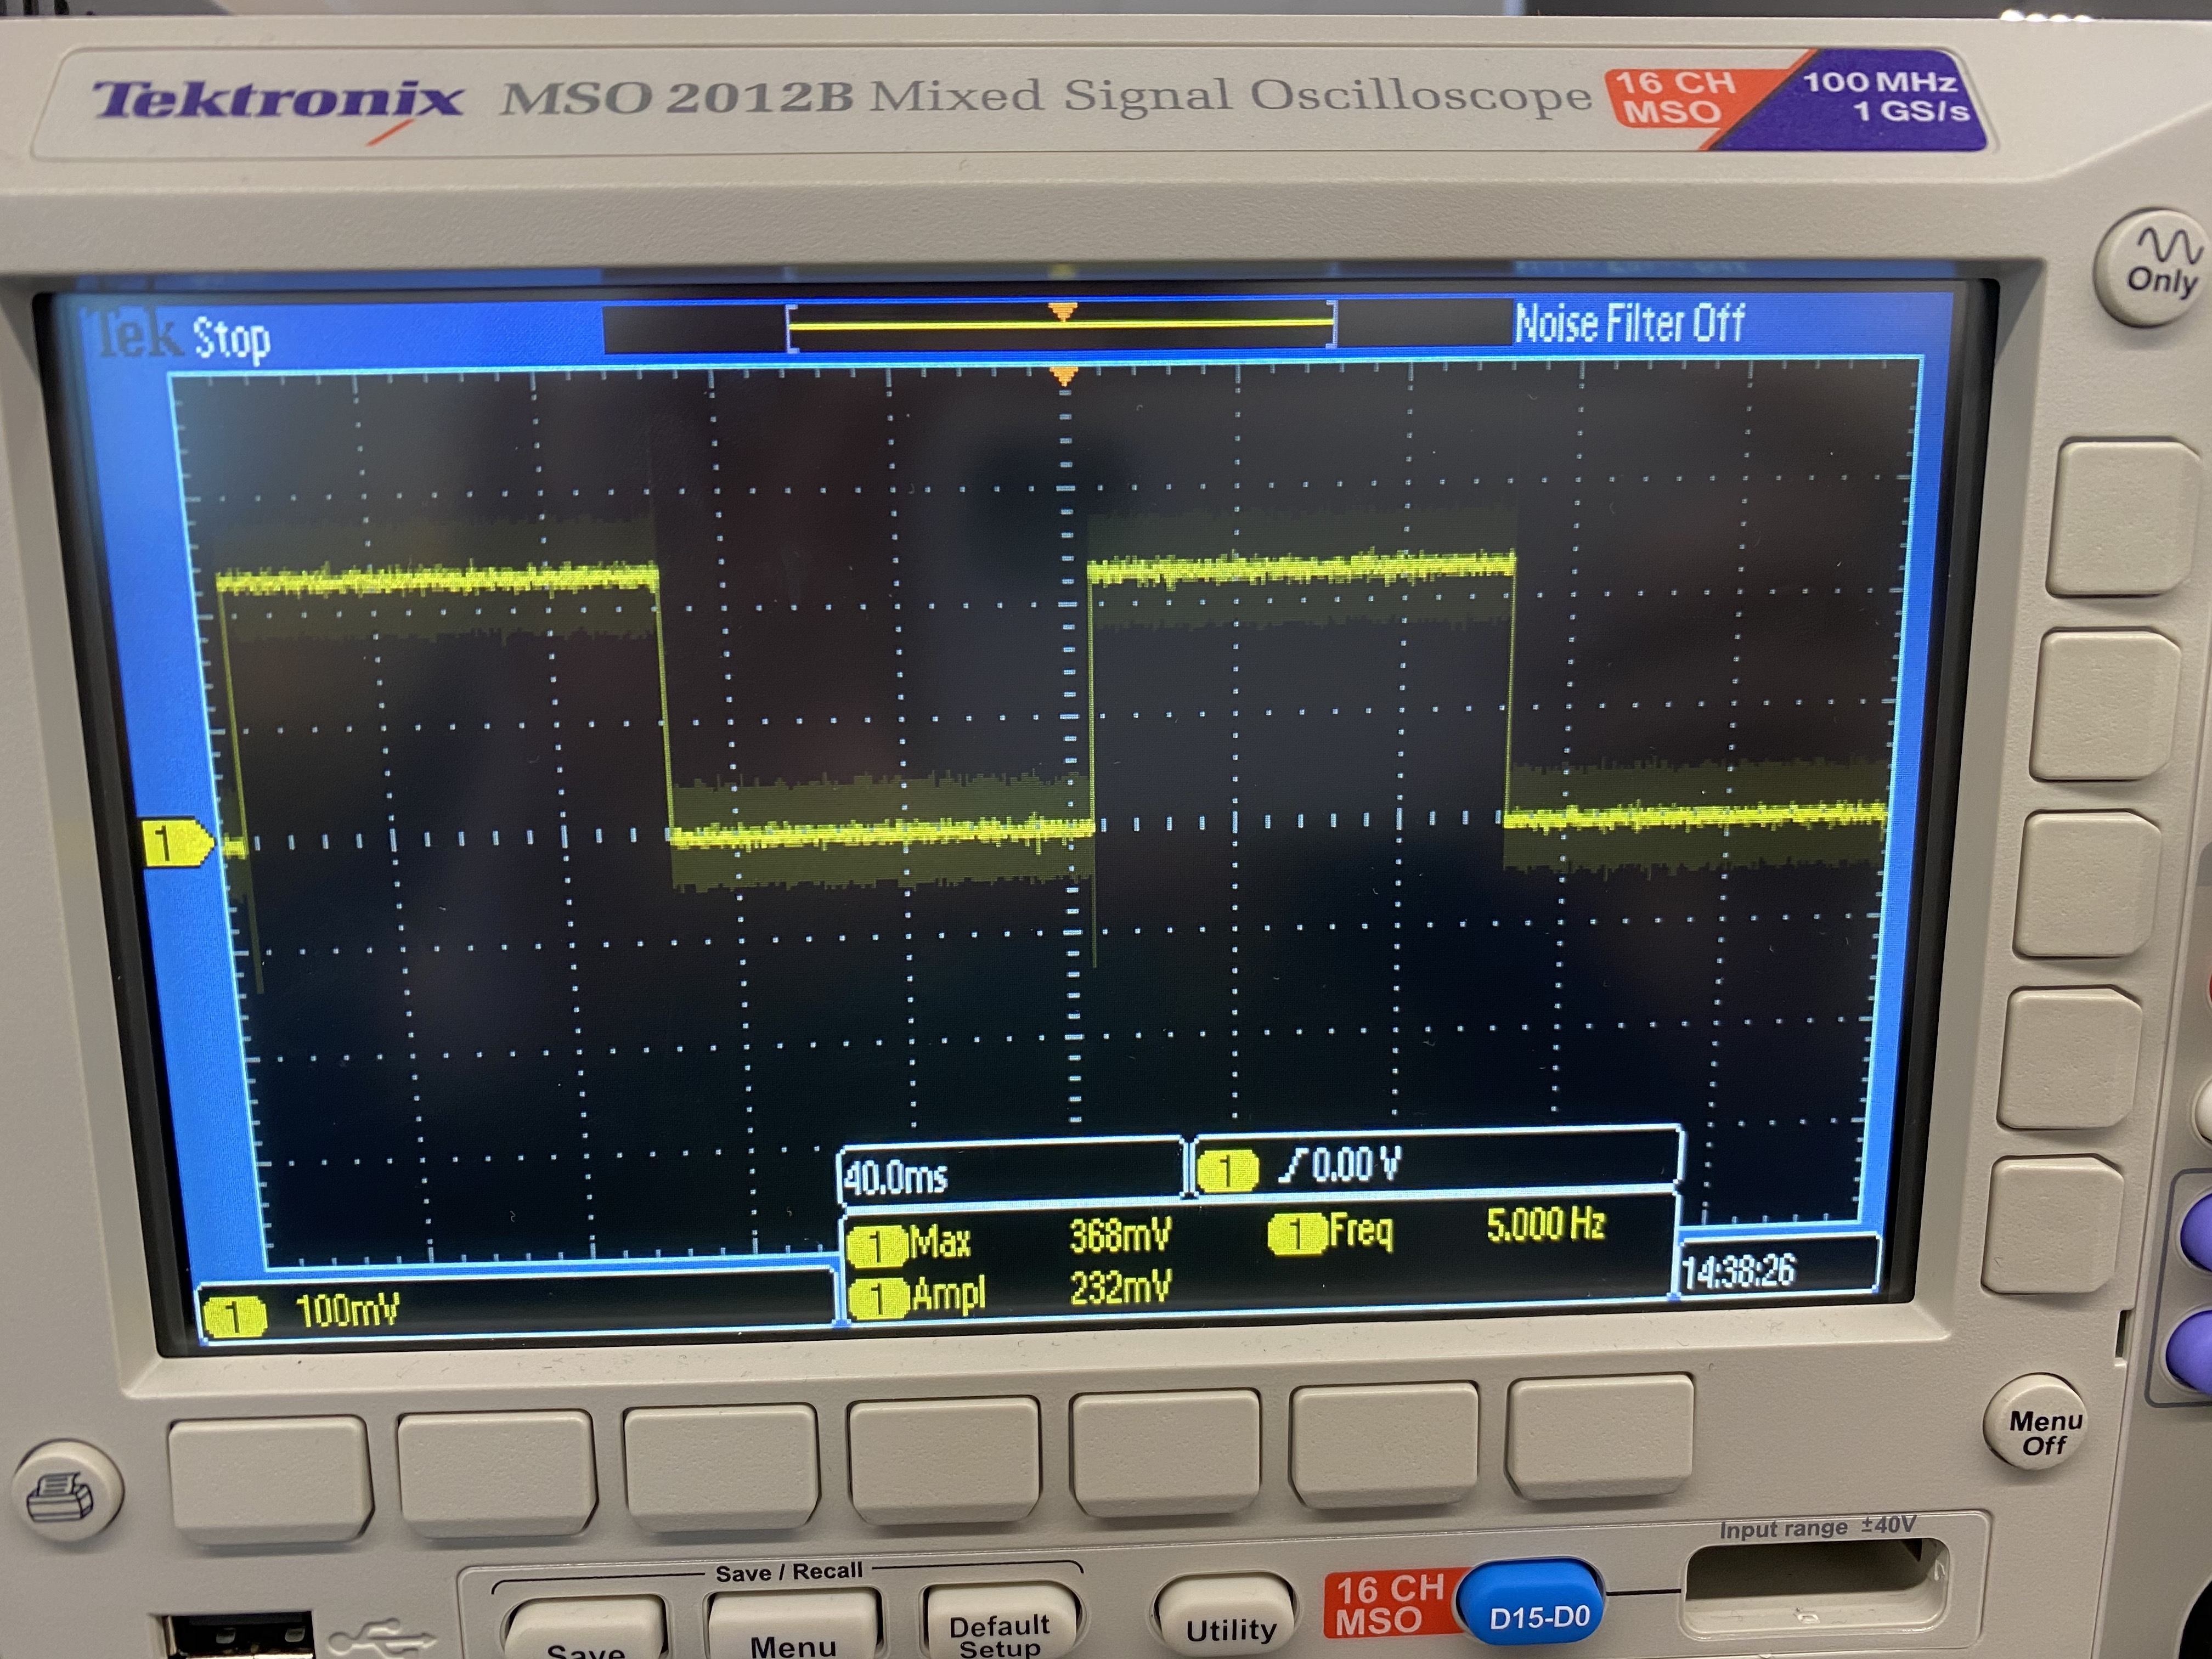
\includegraphics[scale=0.1]{LPFTest5Hz.PNG}}
    \caption{LPF test with 5Hz basband signal}
    \label{fig:LPF5}
\end{figure}

\begin{figure}[H]
    \centerline{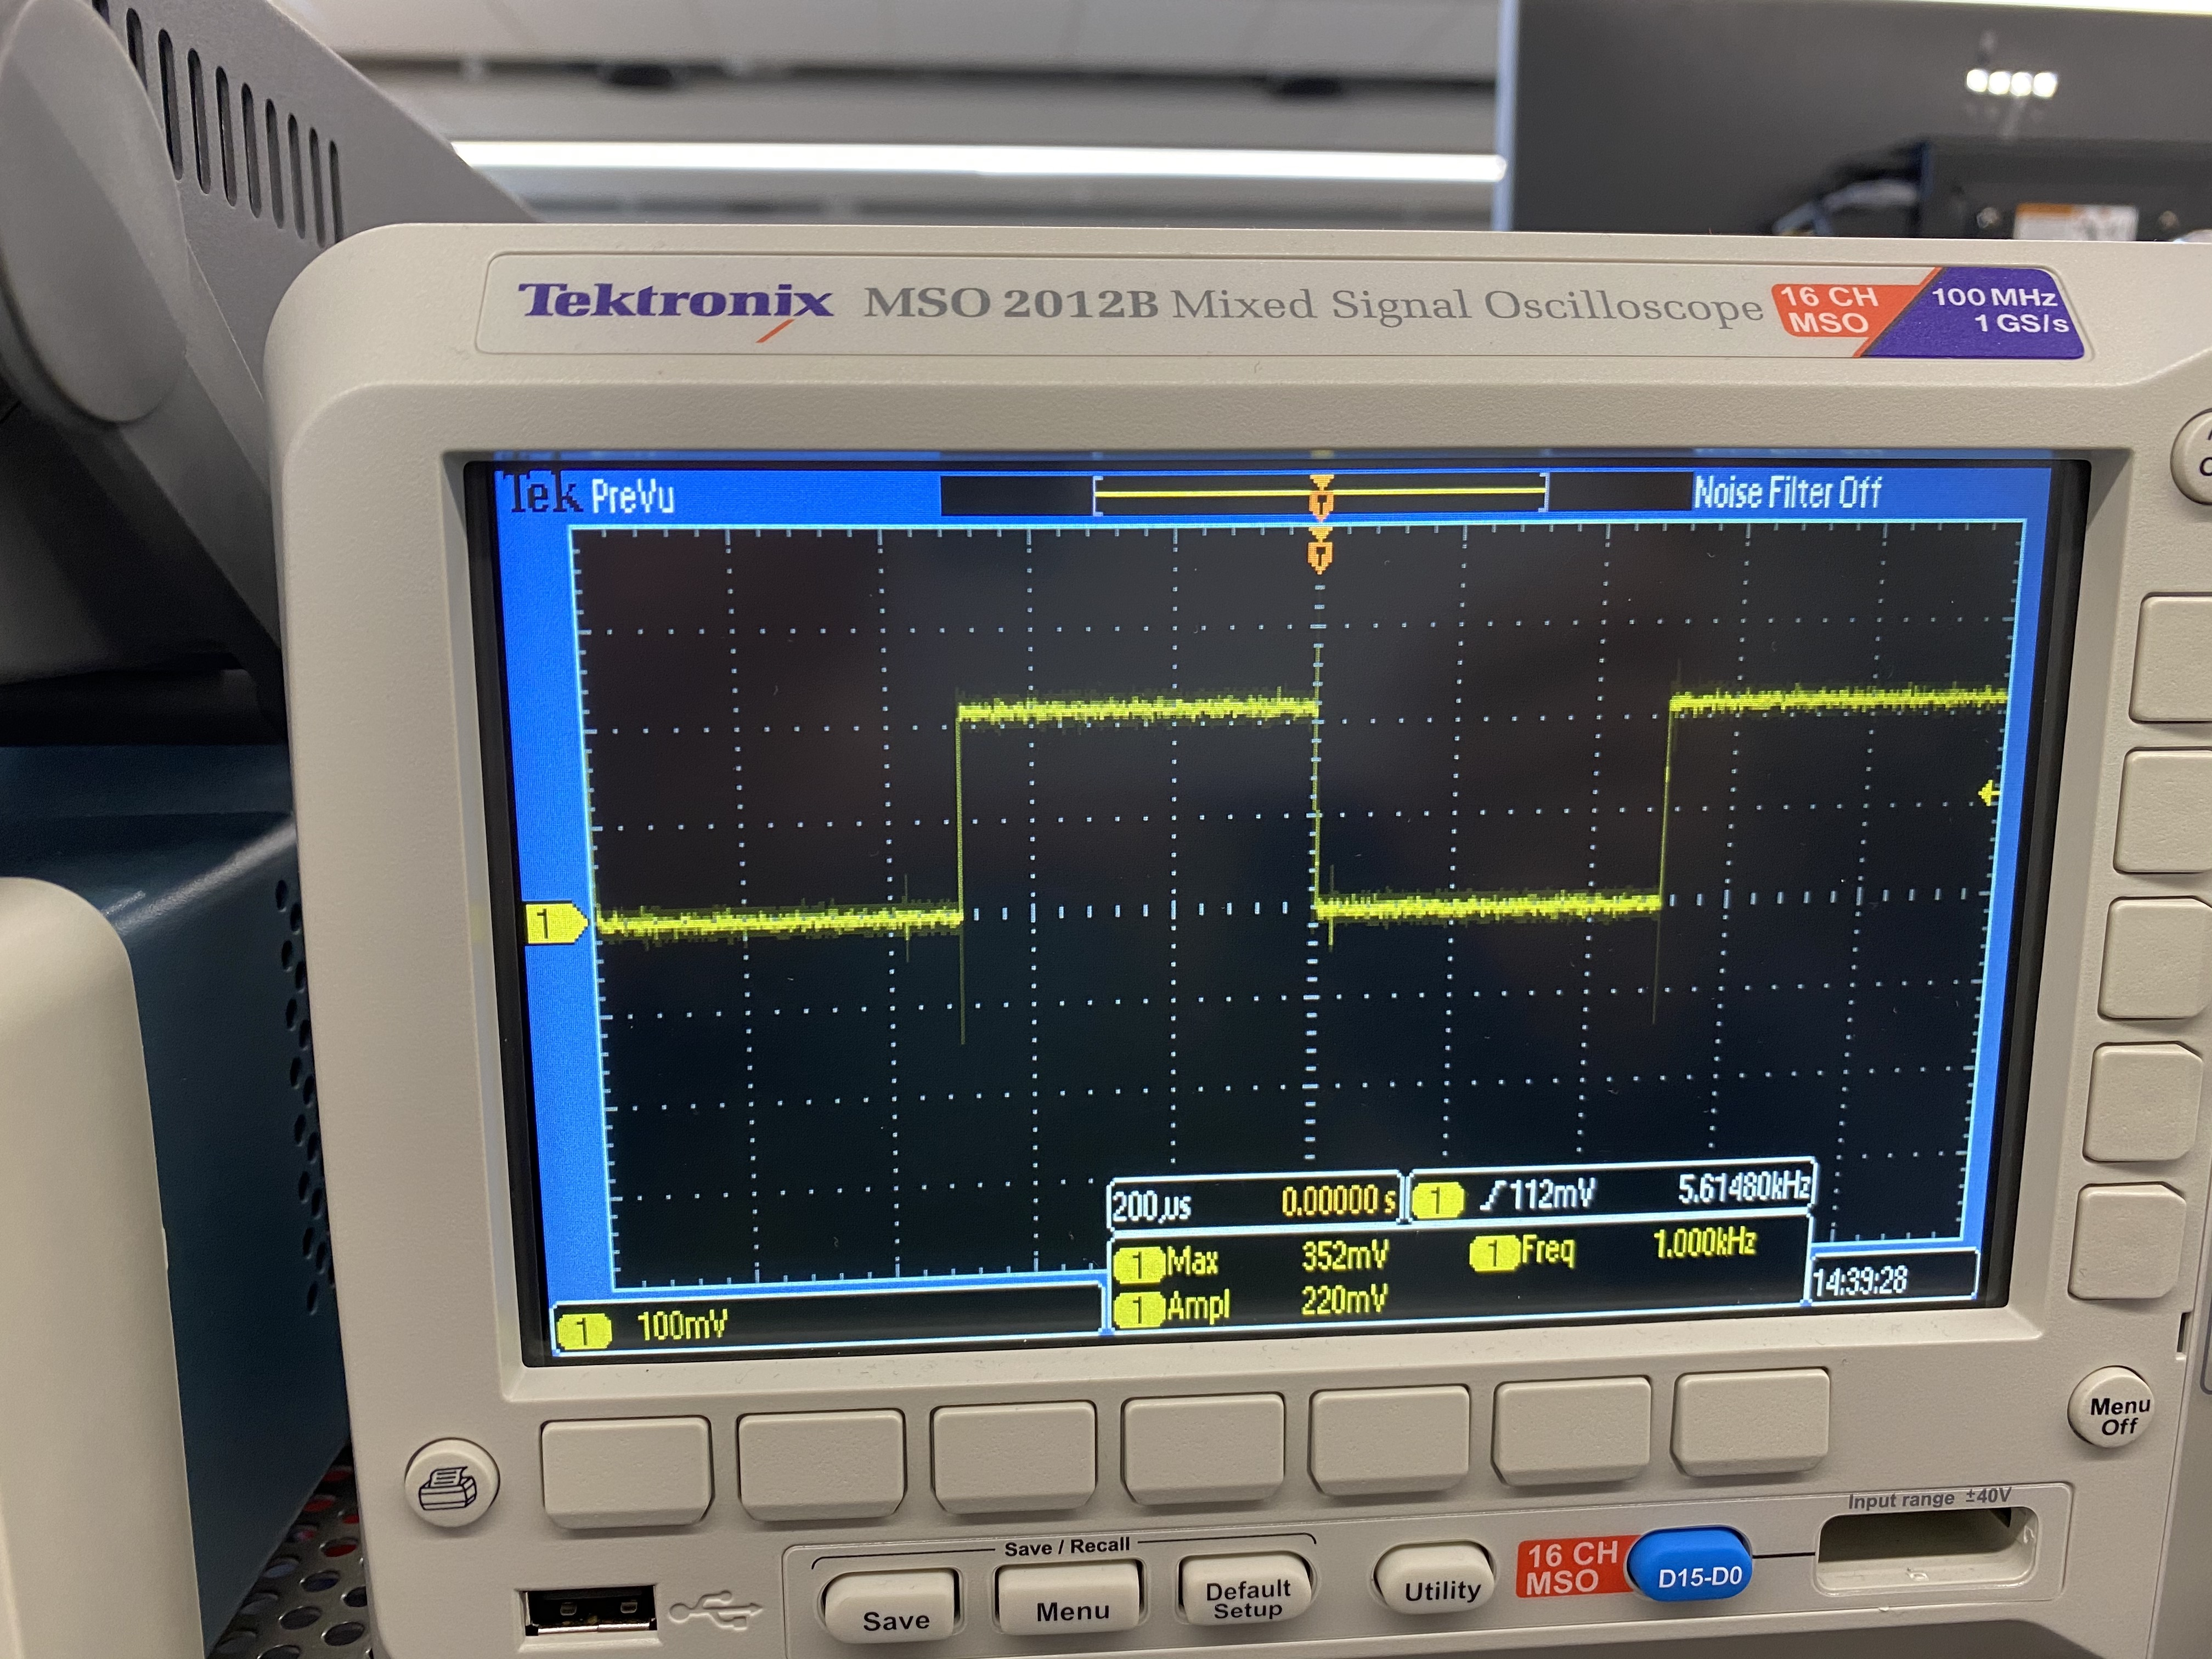
\includegraphics[scale=0.1]{LPFTest1KHz.PNG}}
    \caption{LPF test with 1KHz basband signal}
    \label{fig:LPF1K}
\end{figure}
\chapter{Transmitter's modulator}
% Describe how the output signal from t
The USB FTDI Chip is modulating the provided Voltage
% Controlled Oscillator (VCO).
The modulator has two parts: an op amp and an oscillator. The op amp was connected to the output port of FTDI chip, it amplified the TTL voltage level (0 - 3.3V) to a level which can make the oscillator working (0 - 10V). Followed by the op amp is the oscillator, which was controlled by two voltages: the Vcc port which was connected to the op amp, and the Vin which is connected to a voltage source to provide a voltage which let the oscillator operation in 2.45 GHz.
Under such configuration, the output from the oscillator is: 2.45GHz waveform with Vpp 10V to represent a bit 1, 0 V to represent a bit 0.

The device used is \textbf{ZX95-3000W+}, which is a wide band voltage controlled oscillator. The data sheet can be found at \href{https://www.minicircuits.com/pdfs/ZX95-3000W+.pdf}{MiniCircuit}.

\begin{figure}[ht]
    \centerline{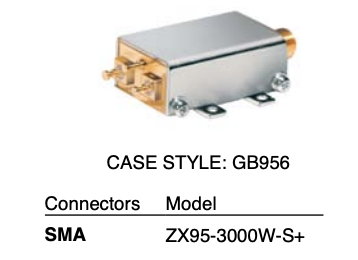
\includegraphics[scale=1.5]{osc}}
    \caption{ZX95-3000W+ oscillator}
    \label{fig:osc}
\end{figure}

\chapter{Entire system testing}
As it is depicted in \hyperref[fig:system_structure]{Figure \ref*{fig:system_structure}}, the signal start from the PC at the transmitter, amplified by the op amp, then modulated to be envelopes and sent by the antenna. This is the transmitter part of the wireless communication system. The microwave is received by the antenna at the receiver part, and it is amplified by the op amp to be detectable enough, filtered and rectified by the rectifier, finally received by the PC at the receiver part.

\begin{figure}[ht]
    
\begin{tikzpicture}
    \tikzstyle{cell} = [rectangle, rounded corners, minimum width=1.8cm, minimum height=1cm,text centered, draw=black, fill=gray!30]
    \node (FTDI) [cell] {Transmitter PC};
    \node (amp) [cell, right = 0.2cm of FTDI.east] {op amp};
    \node (modulator) [cell, right = 0.2cm of amp.east] {modulator};
    \node (transmit) [cell, right = 0.2 cm of modulator.east] {antenna};
    \node (receive) [cell, right = 1.2 cm of transmit.south] {antenna};
    \node (amp2) [cell, right = 0.2cm of receive.east] {op amp};
    \node (detector) [cell, right = 0.2cm of amp2.east] {rectifier};
    \node (rec) [cell, right = 0.2cm of detector.east] {receiver PC};
    
    \draw (FTDI) -- (amp);
    \draw (amp) -- (modulator);
    \draw (modulator) -- (transmit);
    \draw (receive) -- (amp2);
    \draw (amp2) -- (detector);
    \draw (detector) -- (rec);
\end{tikzpicture}
    \caption{Final structure of the system}
    \label{fig:final_structure}
\end{figure}

The task of testing the entire system is to setup the whole system first, then input something at the transmitter PC, the receiver PC should be able to display what has been typed in the transmitter PC.

Note that it is also possible to check the system availability from the raw bit waveform at the port of PCs of receiver and transmitter.

\begin{figure}[ht]
    \centerline{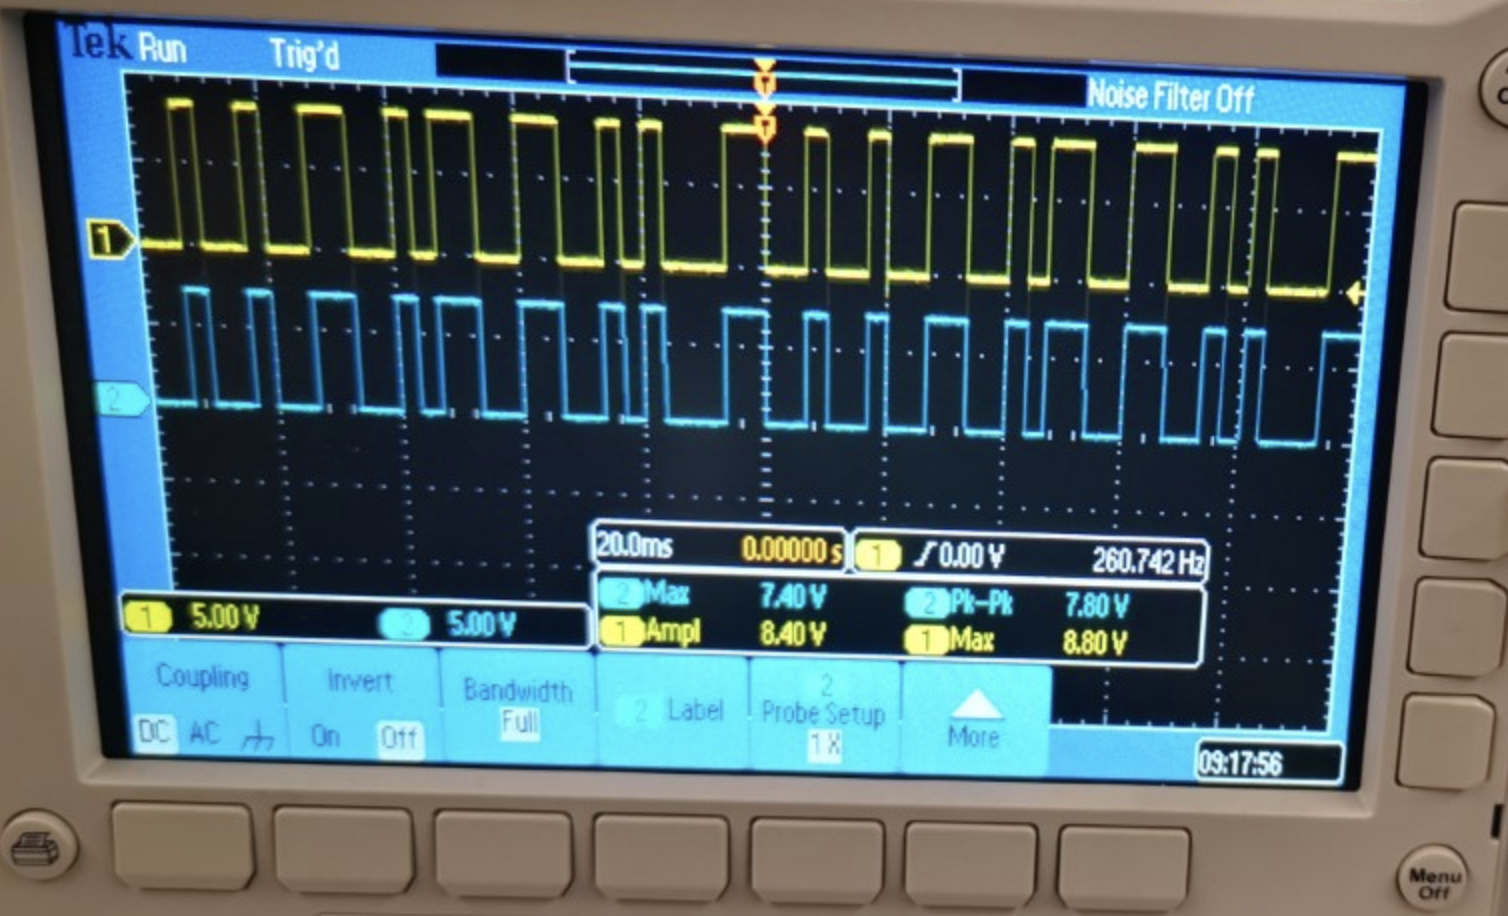
\includegraphics[scale=1]{raw_waveform_compare}}
    \caption{Waveforms at the transmitter PC and the receiver PC}
    \label{fig:raw_bit_waveform}
\end{figure}
% \begin{figure}
%     \centerline{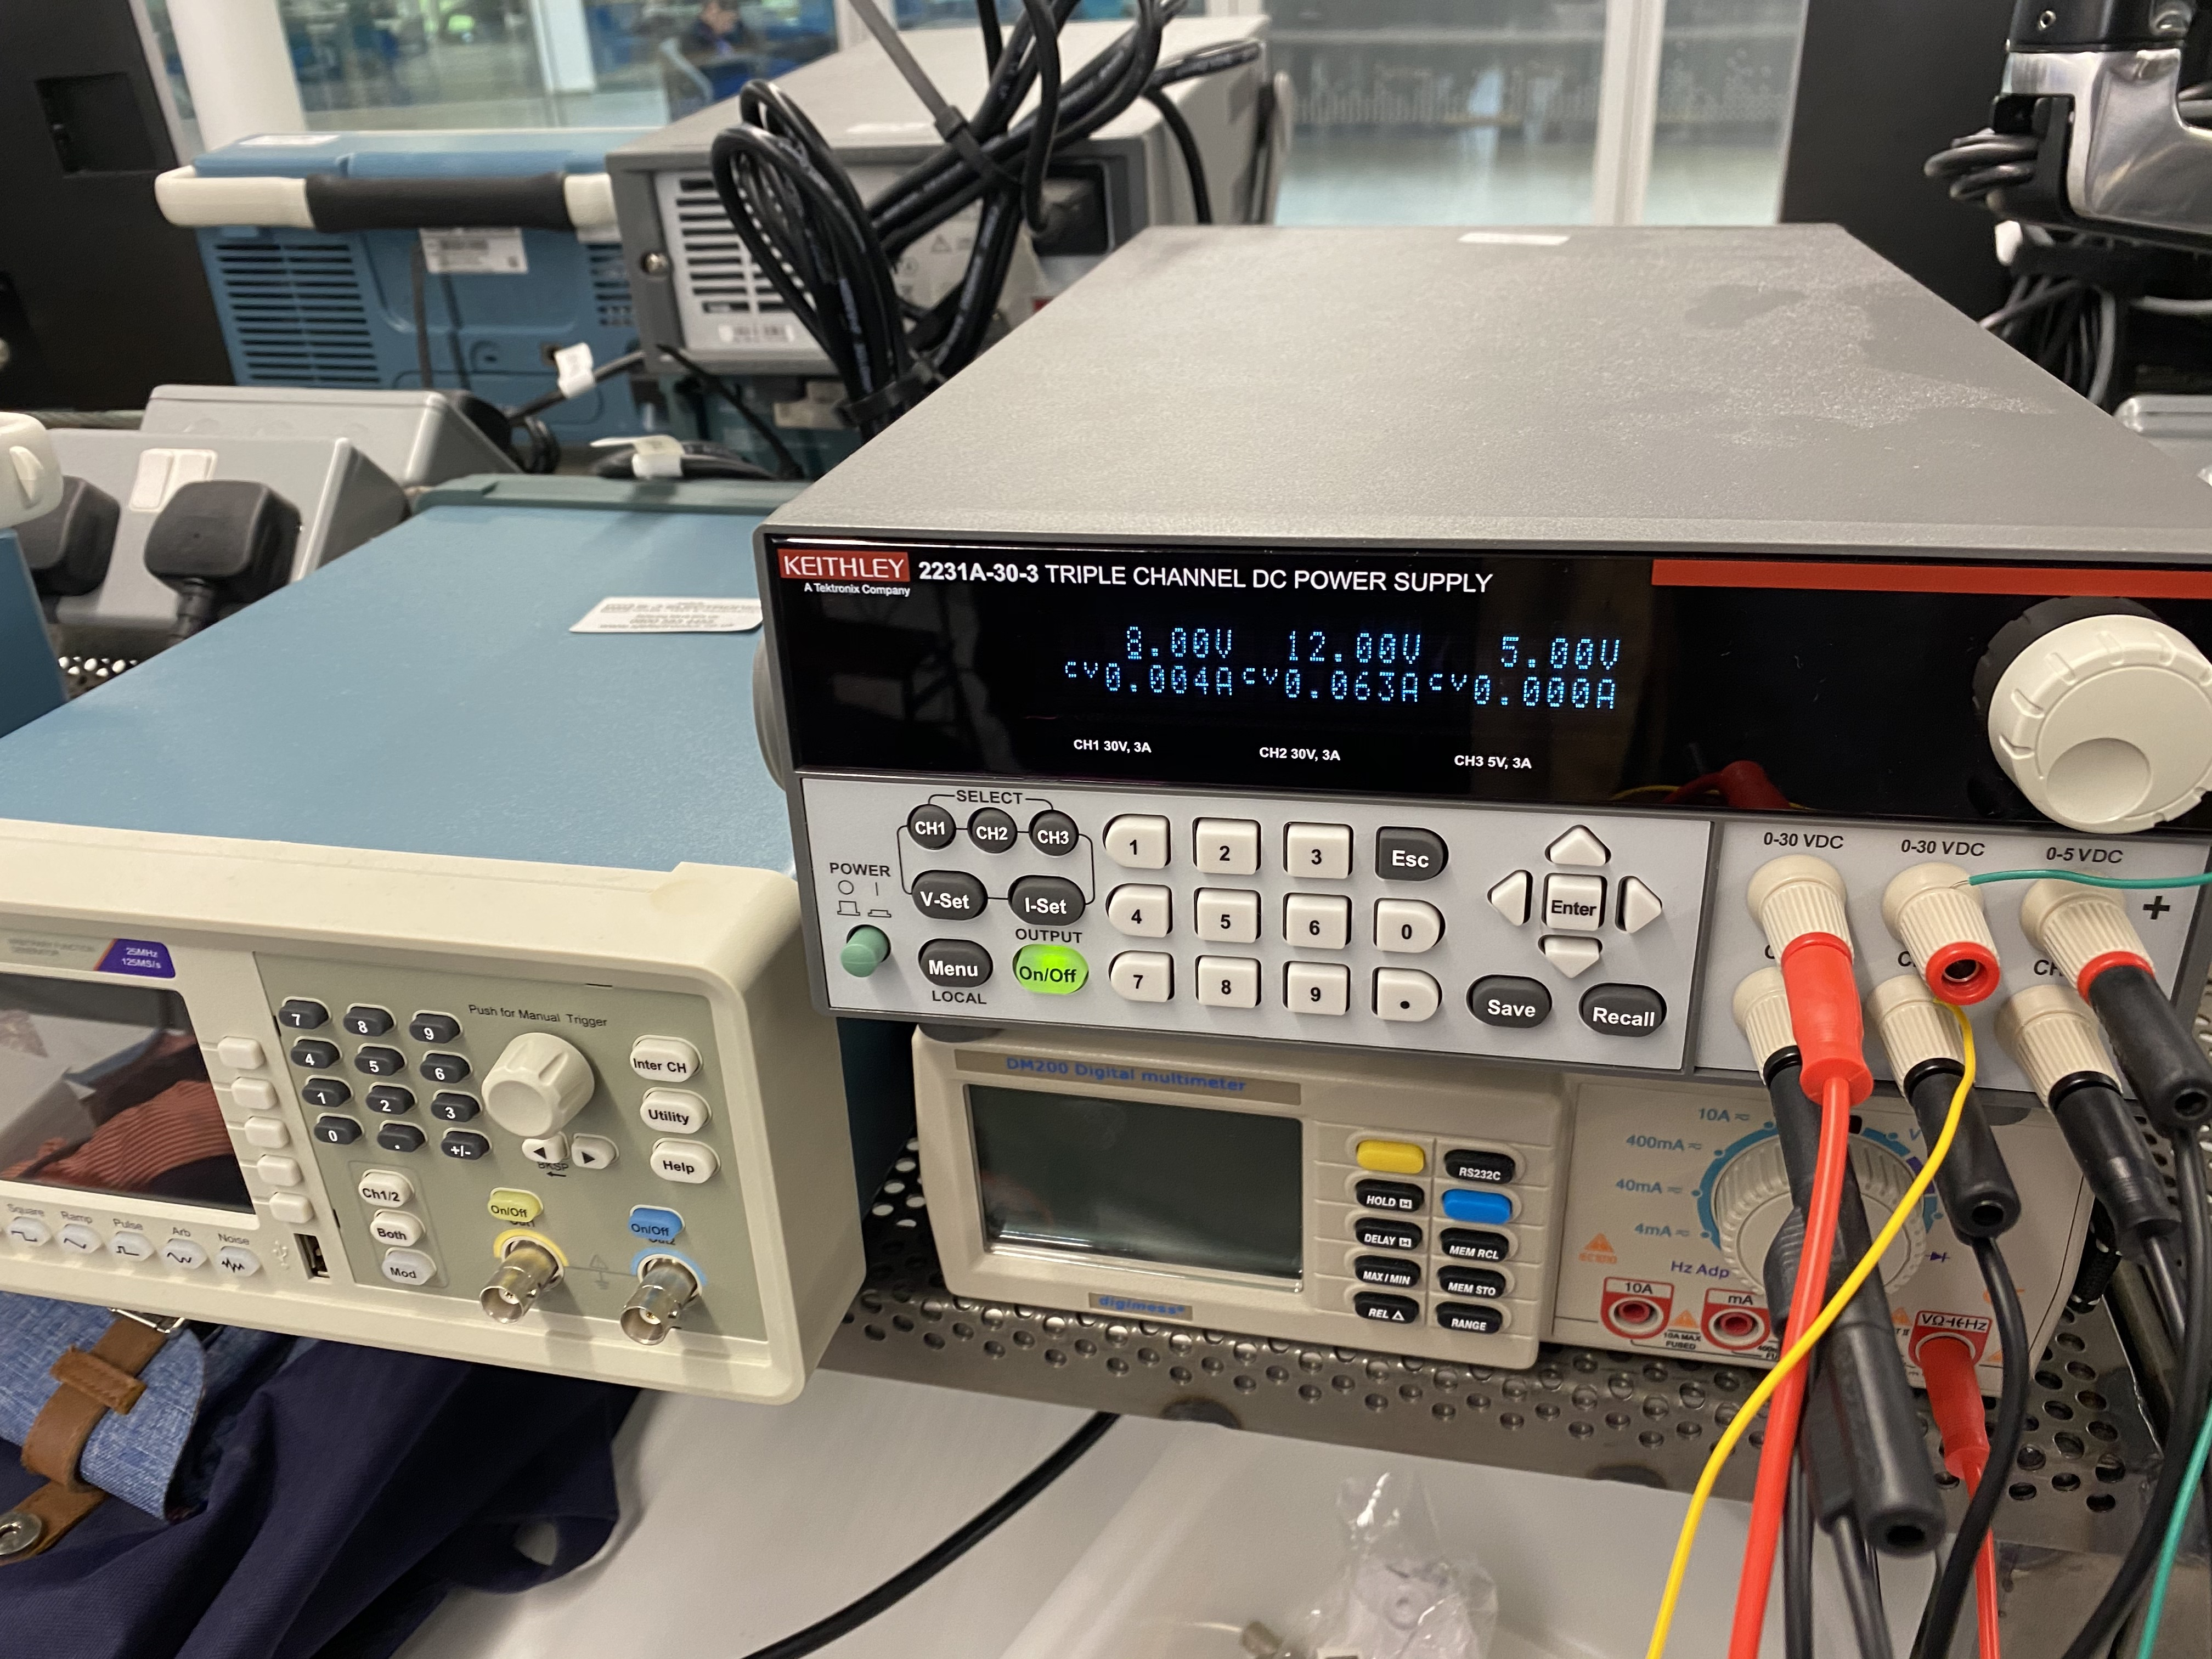
\includegraphics[scale=0.1]{DC_PowerSupplyReceiver.PNG}}
%     \caption{DC power supply at transmitter side}
%     \label{fig:DCT}
% \end{figure}
% \begin{figure}
%     \centerline{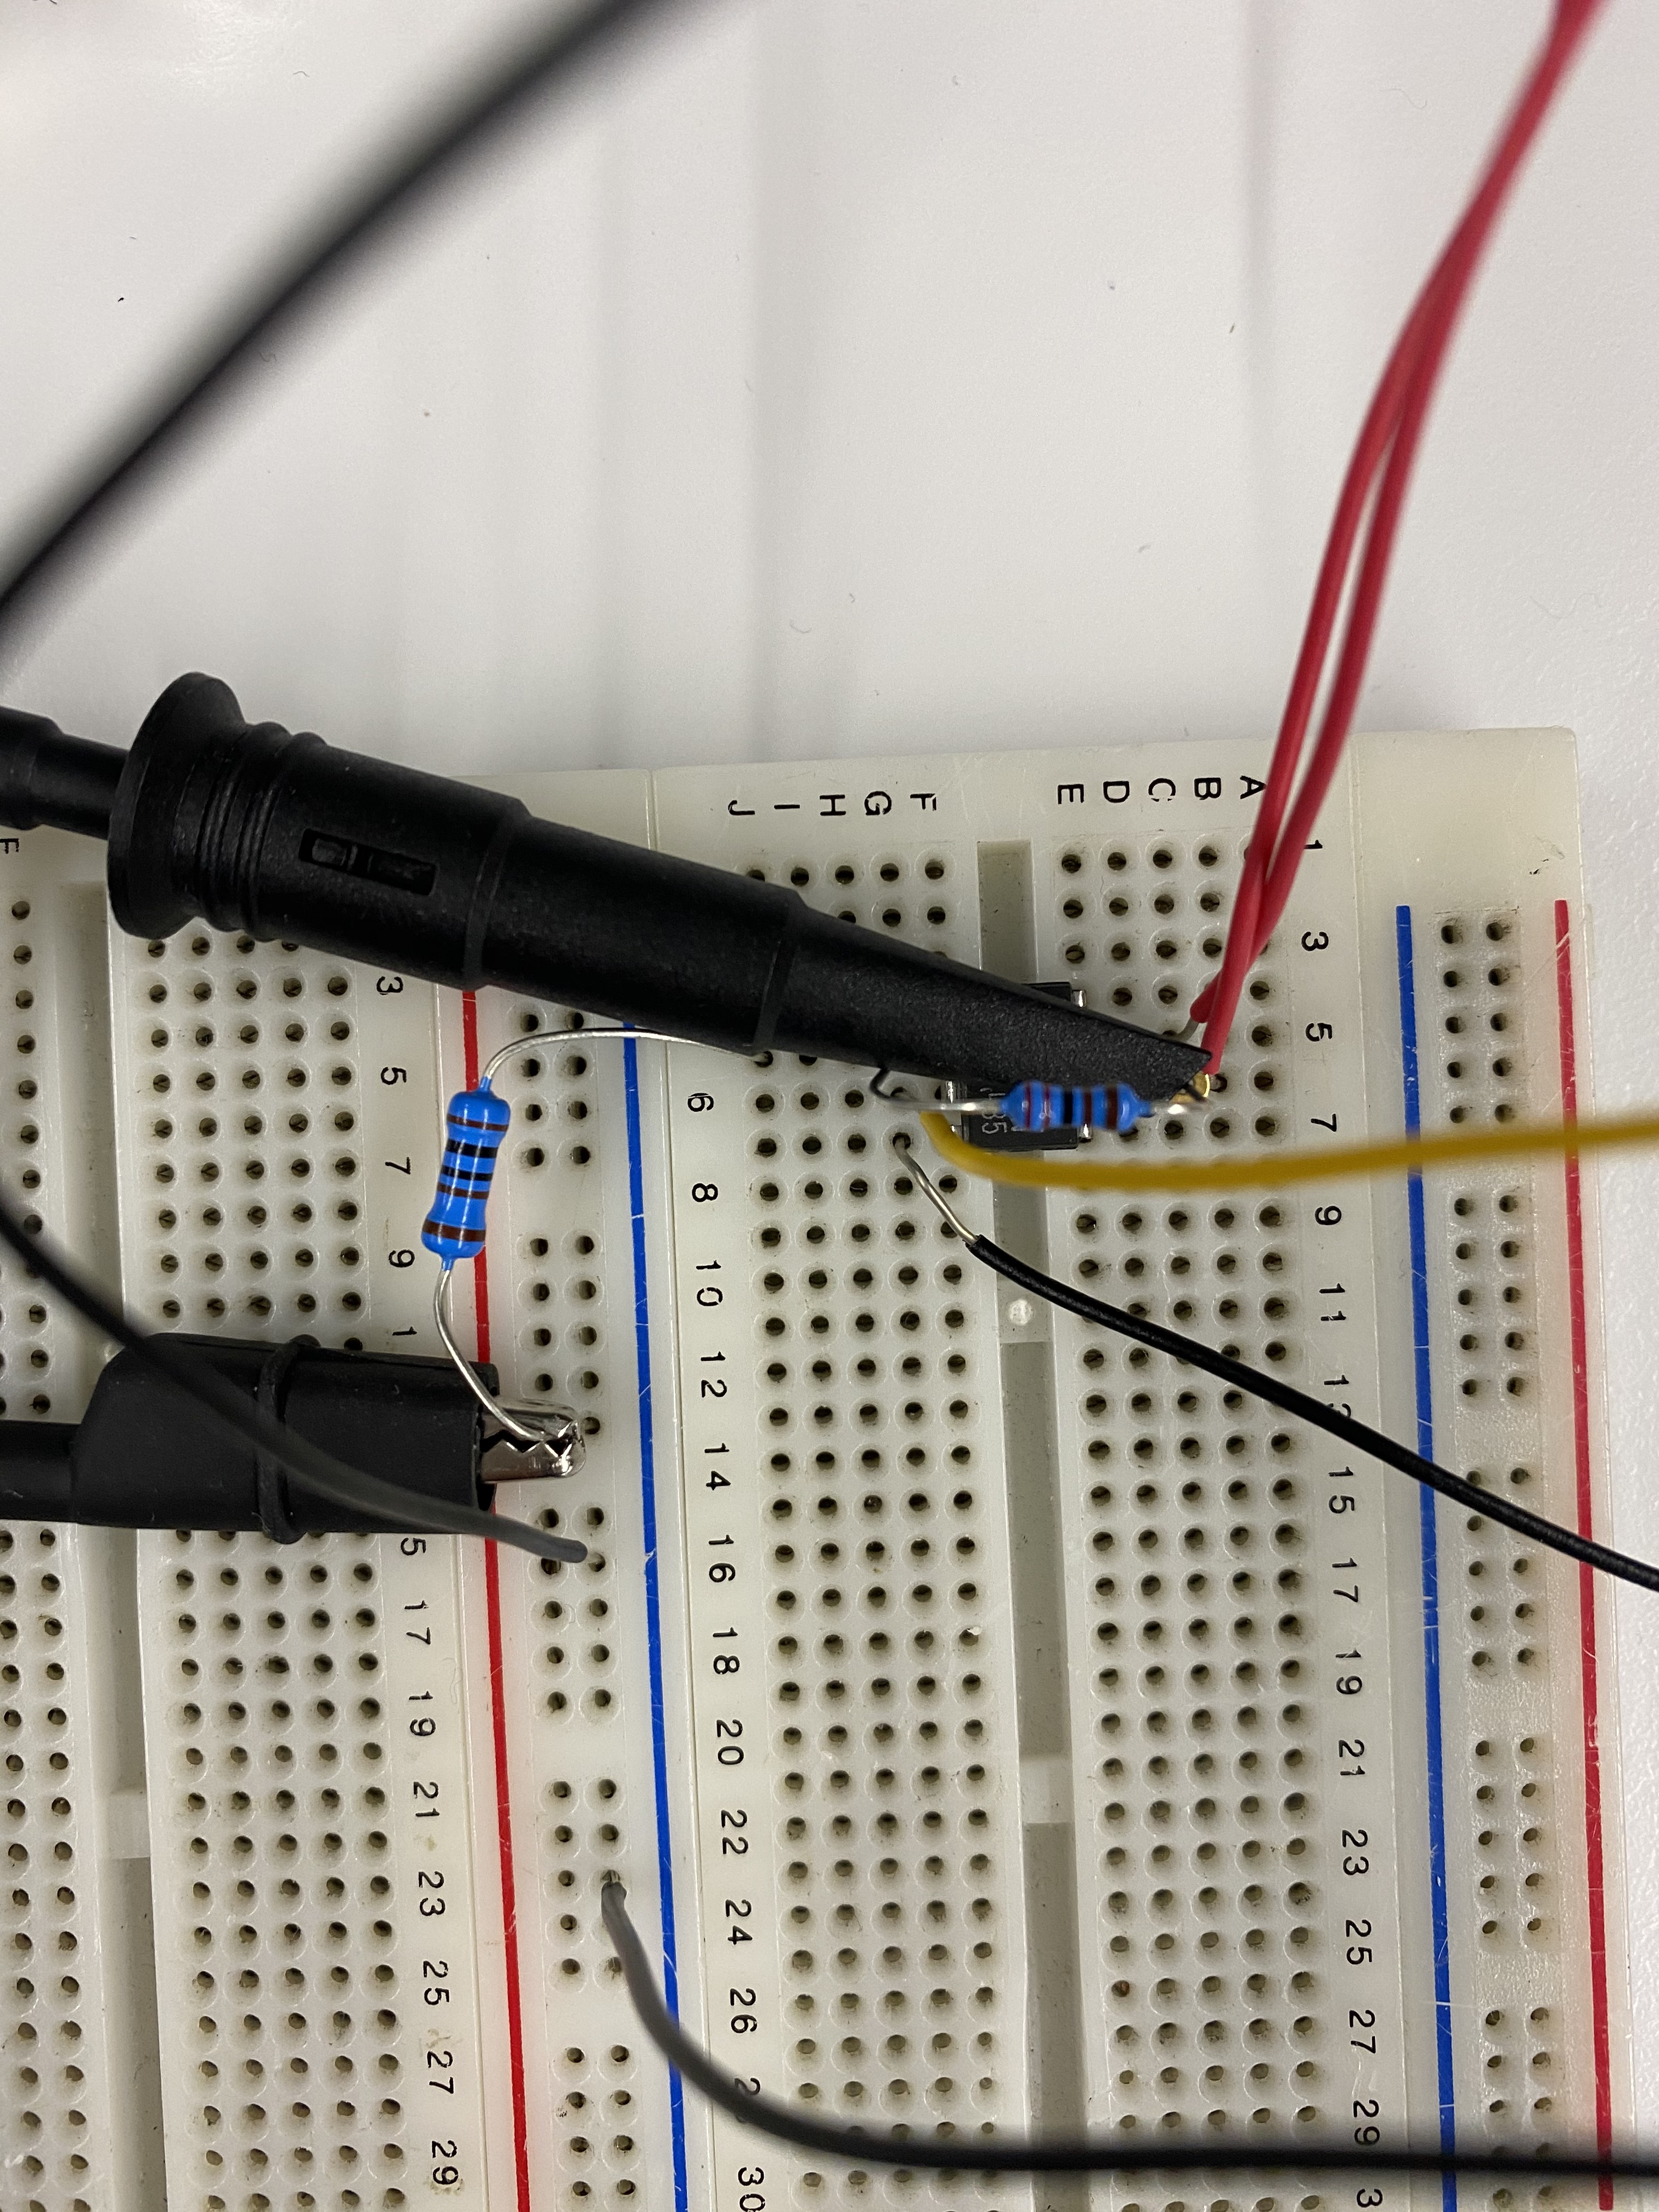
\includegraphics[scale=0.1]{OPAMP_Transmitter.PNG}}
%     \caption{OPAMP at transmitter side}
%     \label{fig:OPAMPT}
% \end{figure}
% \begin{figure}
%     \centerline{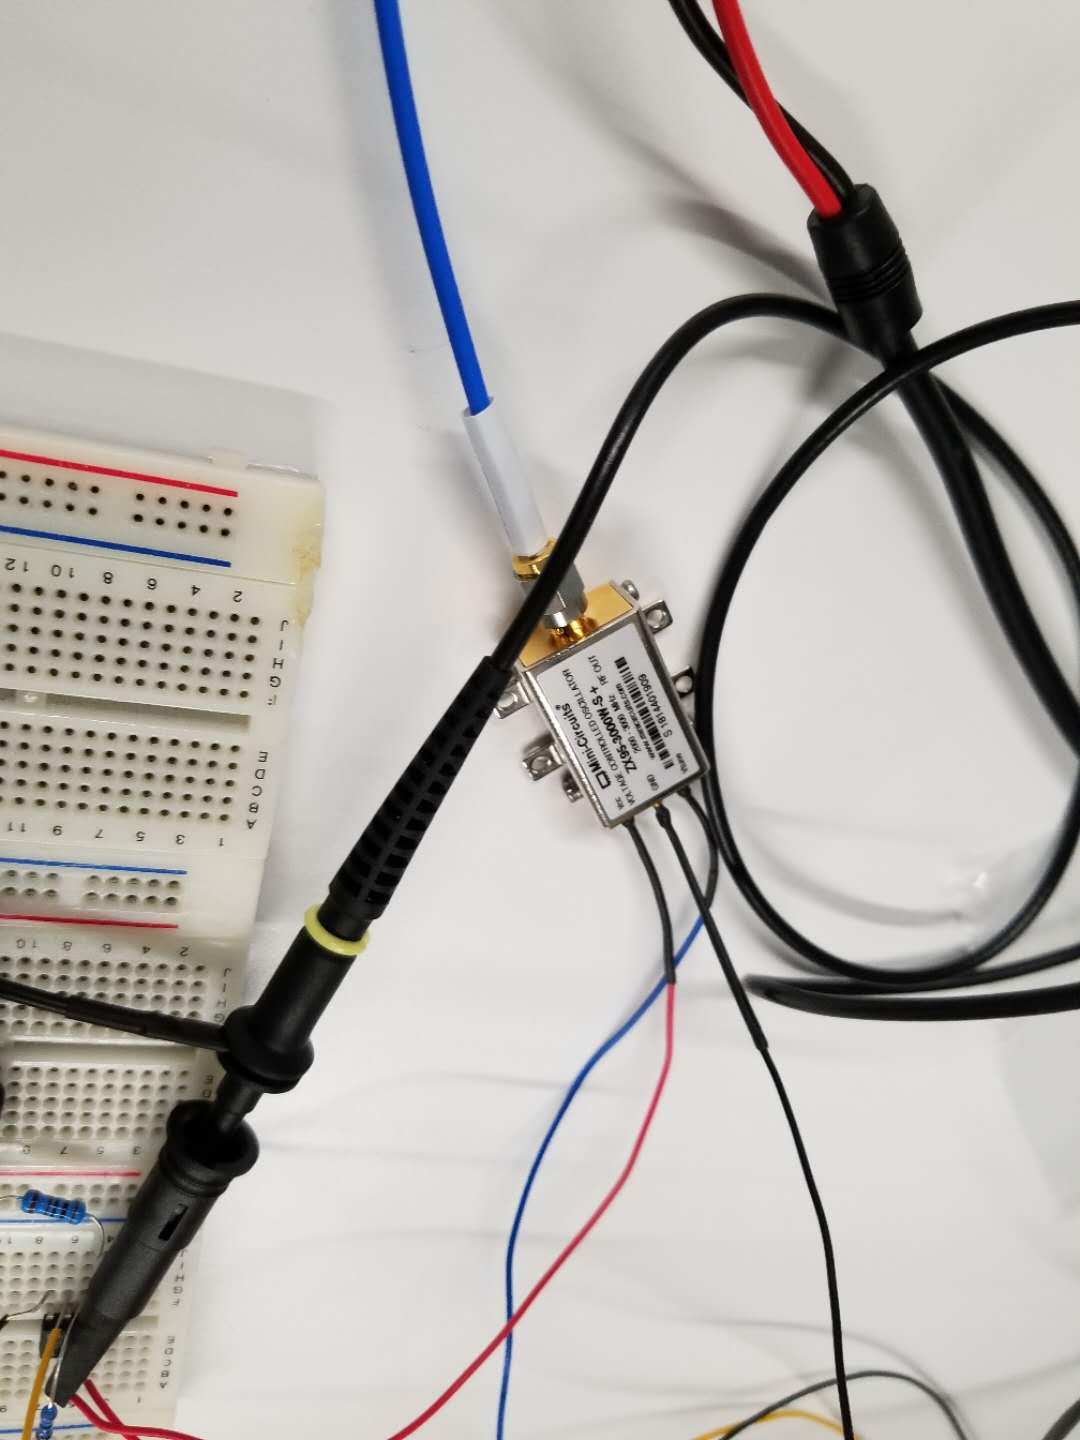
\includegraphics[scale=0.2]{Oscillator.PNG}}
%     \caption{Oscillator}
%     \label{fig:Oscilaltor}
% \end{figure}
% \begin{figure}
%     \centerline{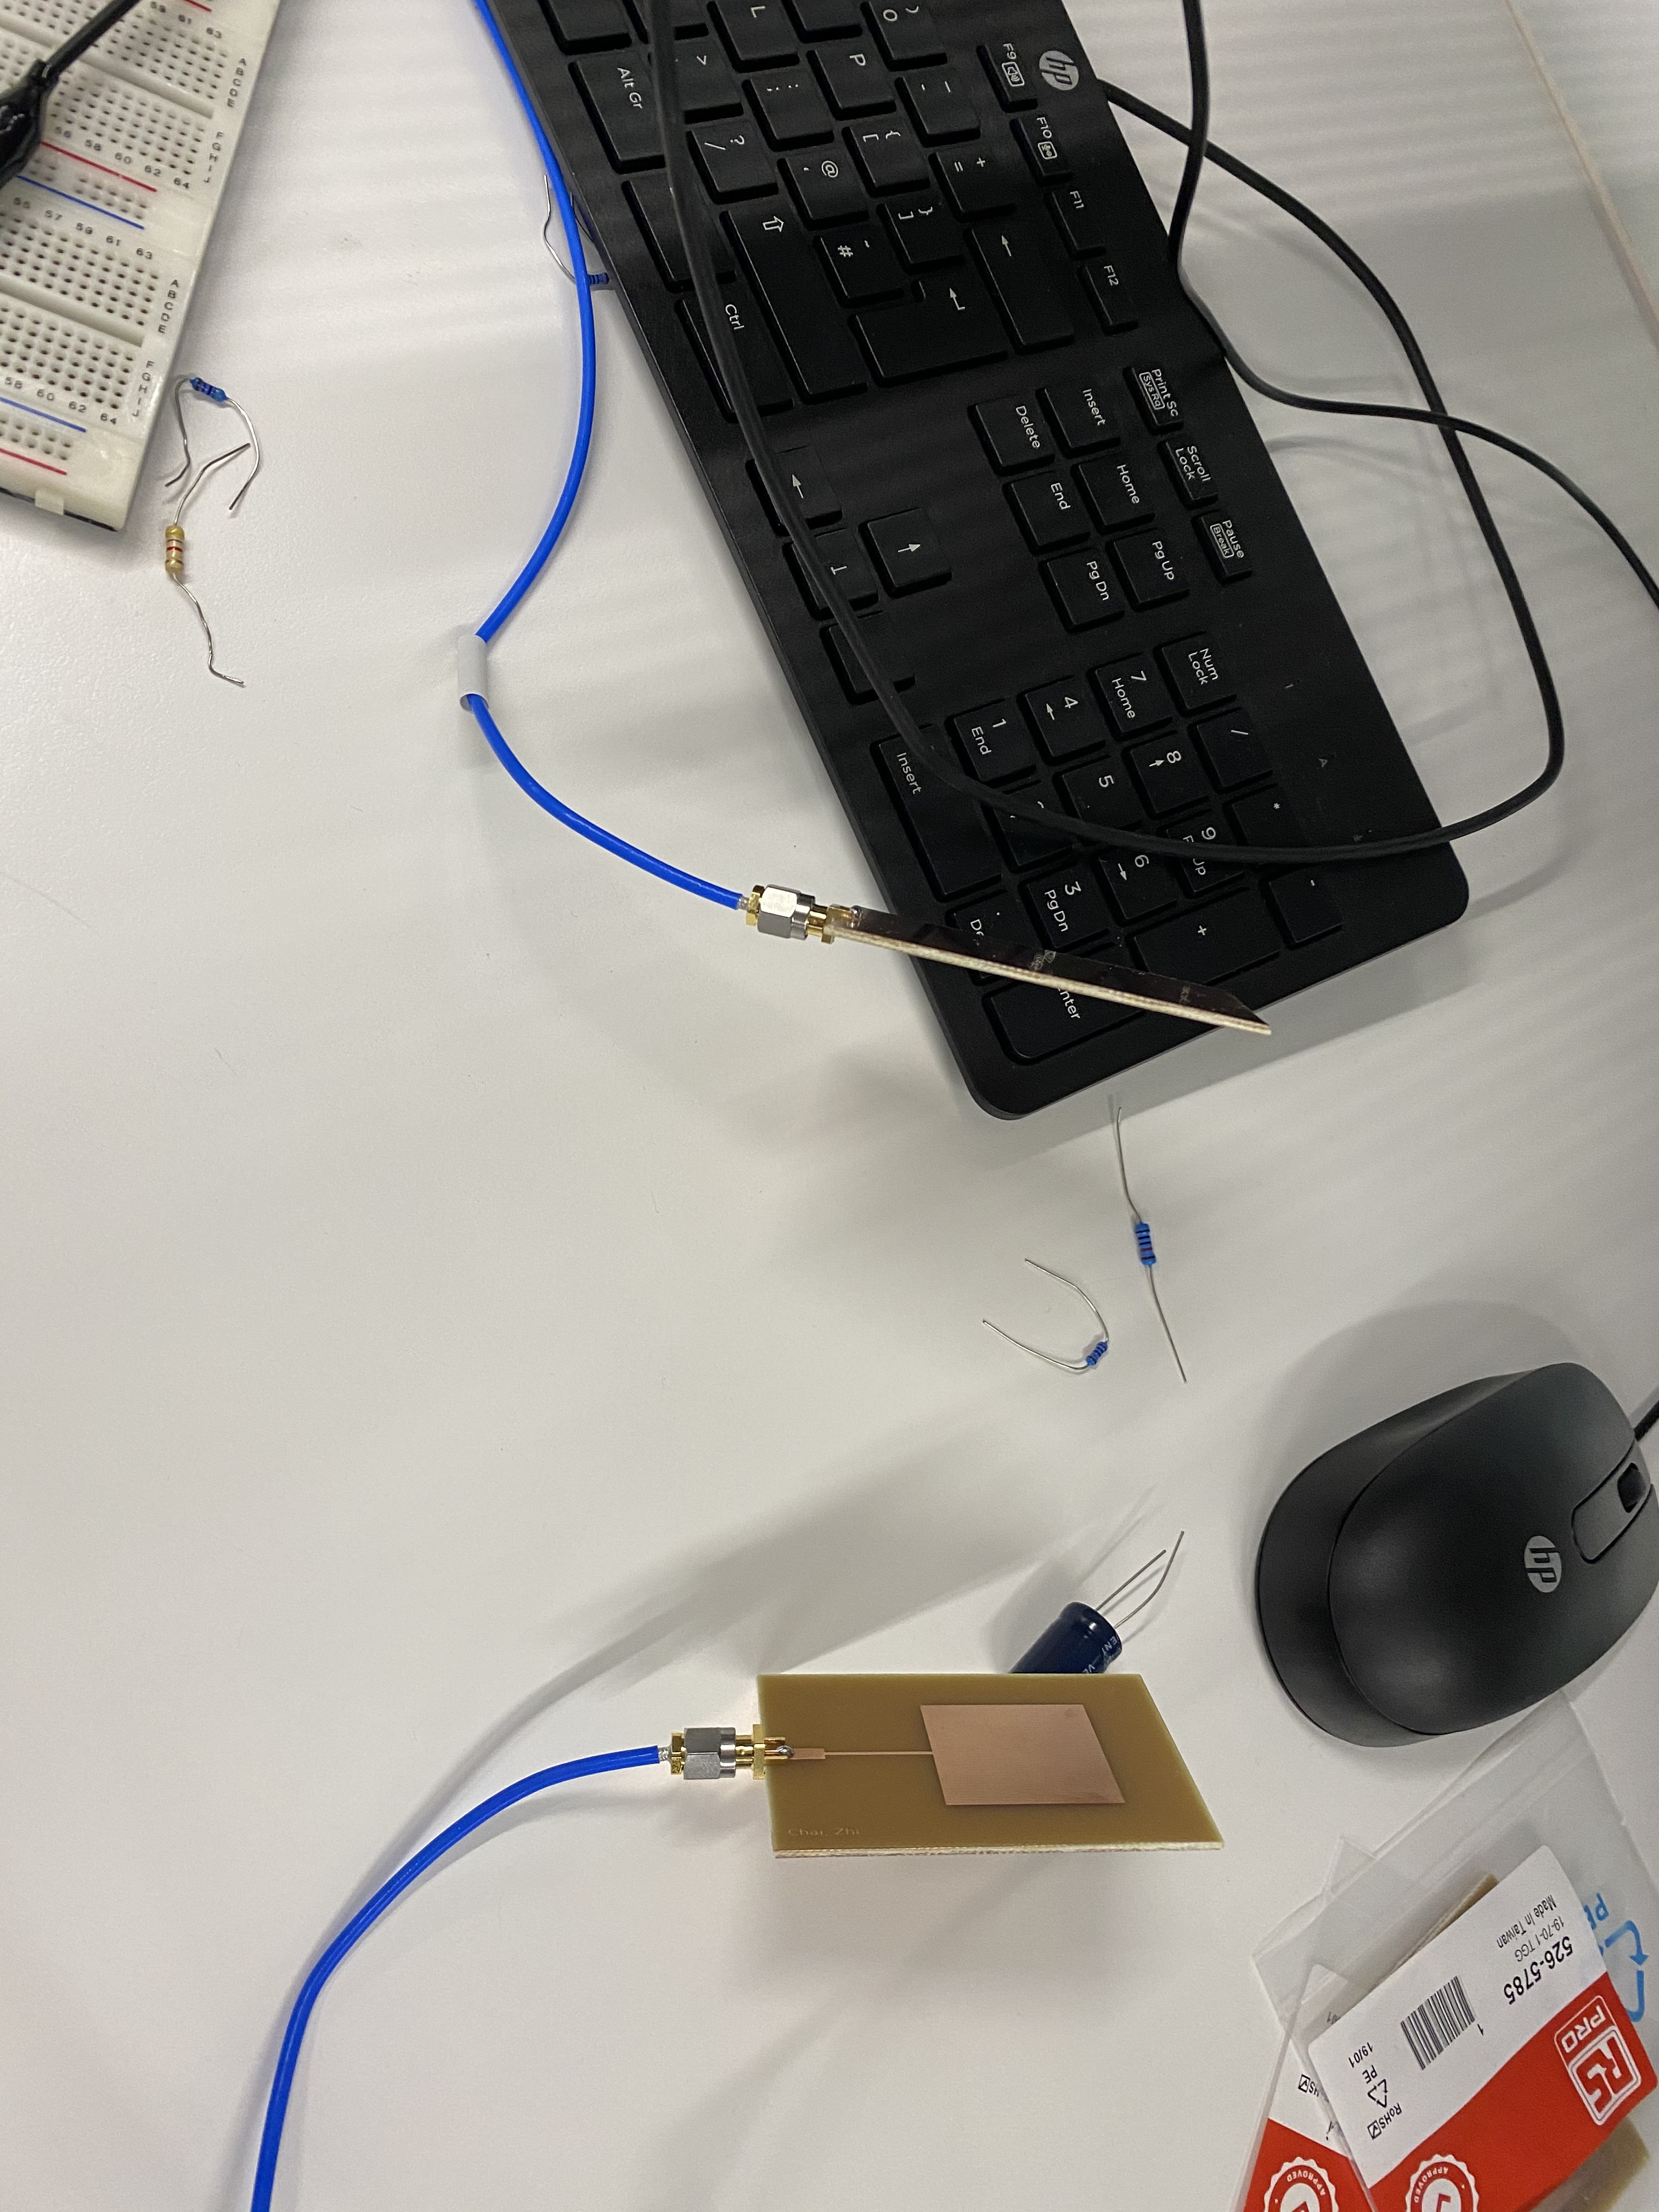
\includegraphics[scale=0.1]{Antennas.PNG}}
%     \caption{Transmitting antenna and receiving antenna}
%     \label{fig:Antennas}
% \end{figure}
% \begin{figure}
%     \centerline{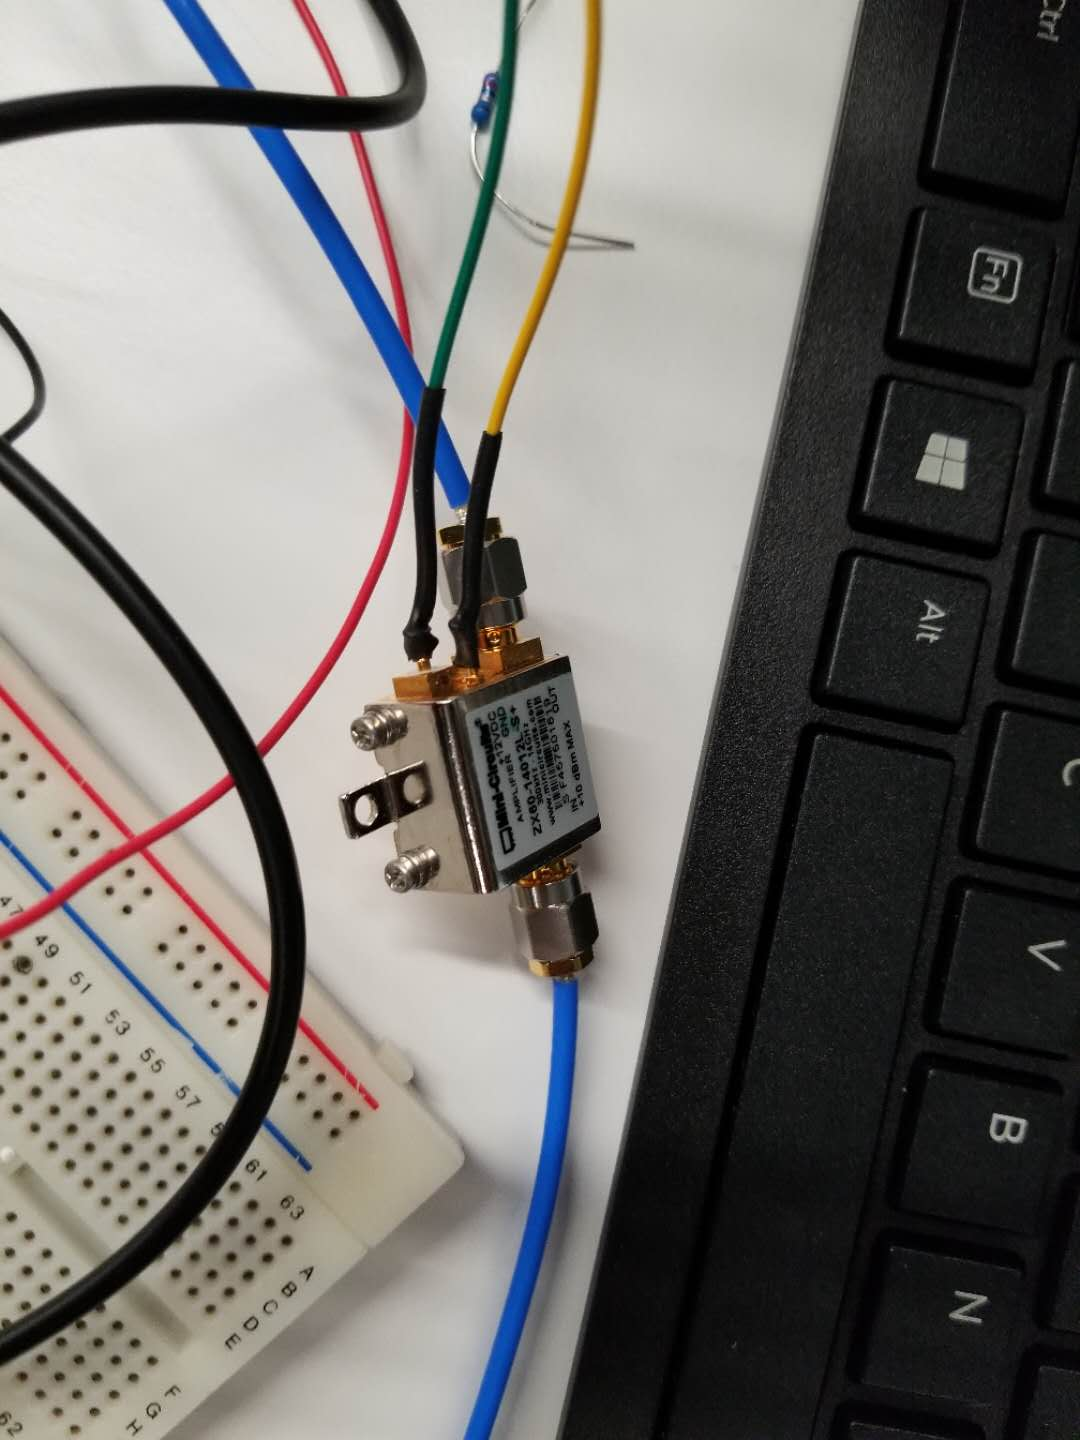
\includegraphics[scale=0.2]{LNA.PNG}}
%     \caption{Low noise amplifier}
%     \label{fig:LNA}
% \end{figure}
% \begin{figure}
%     \centerline{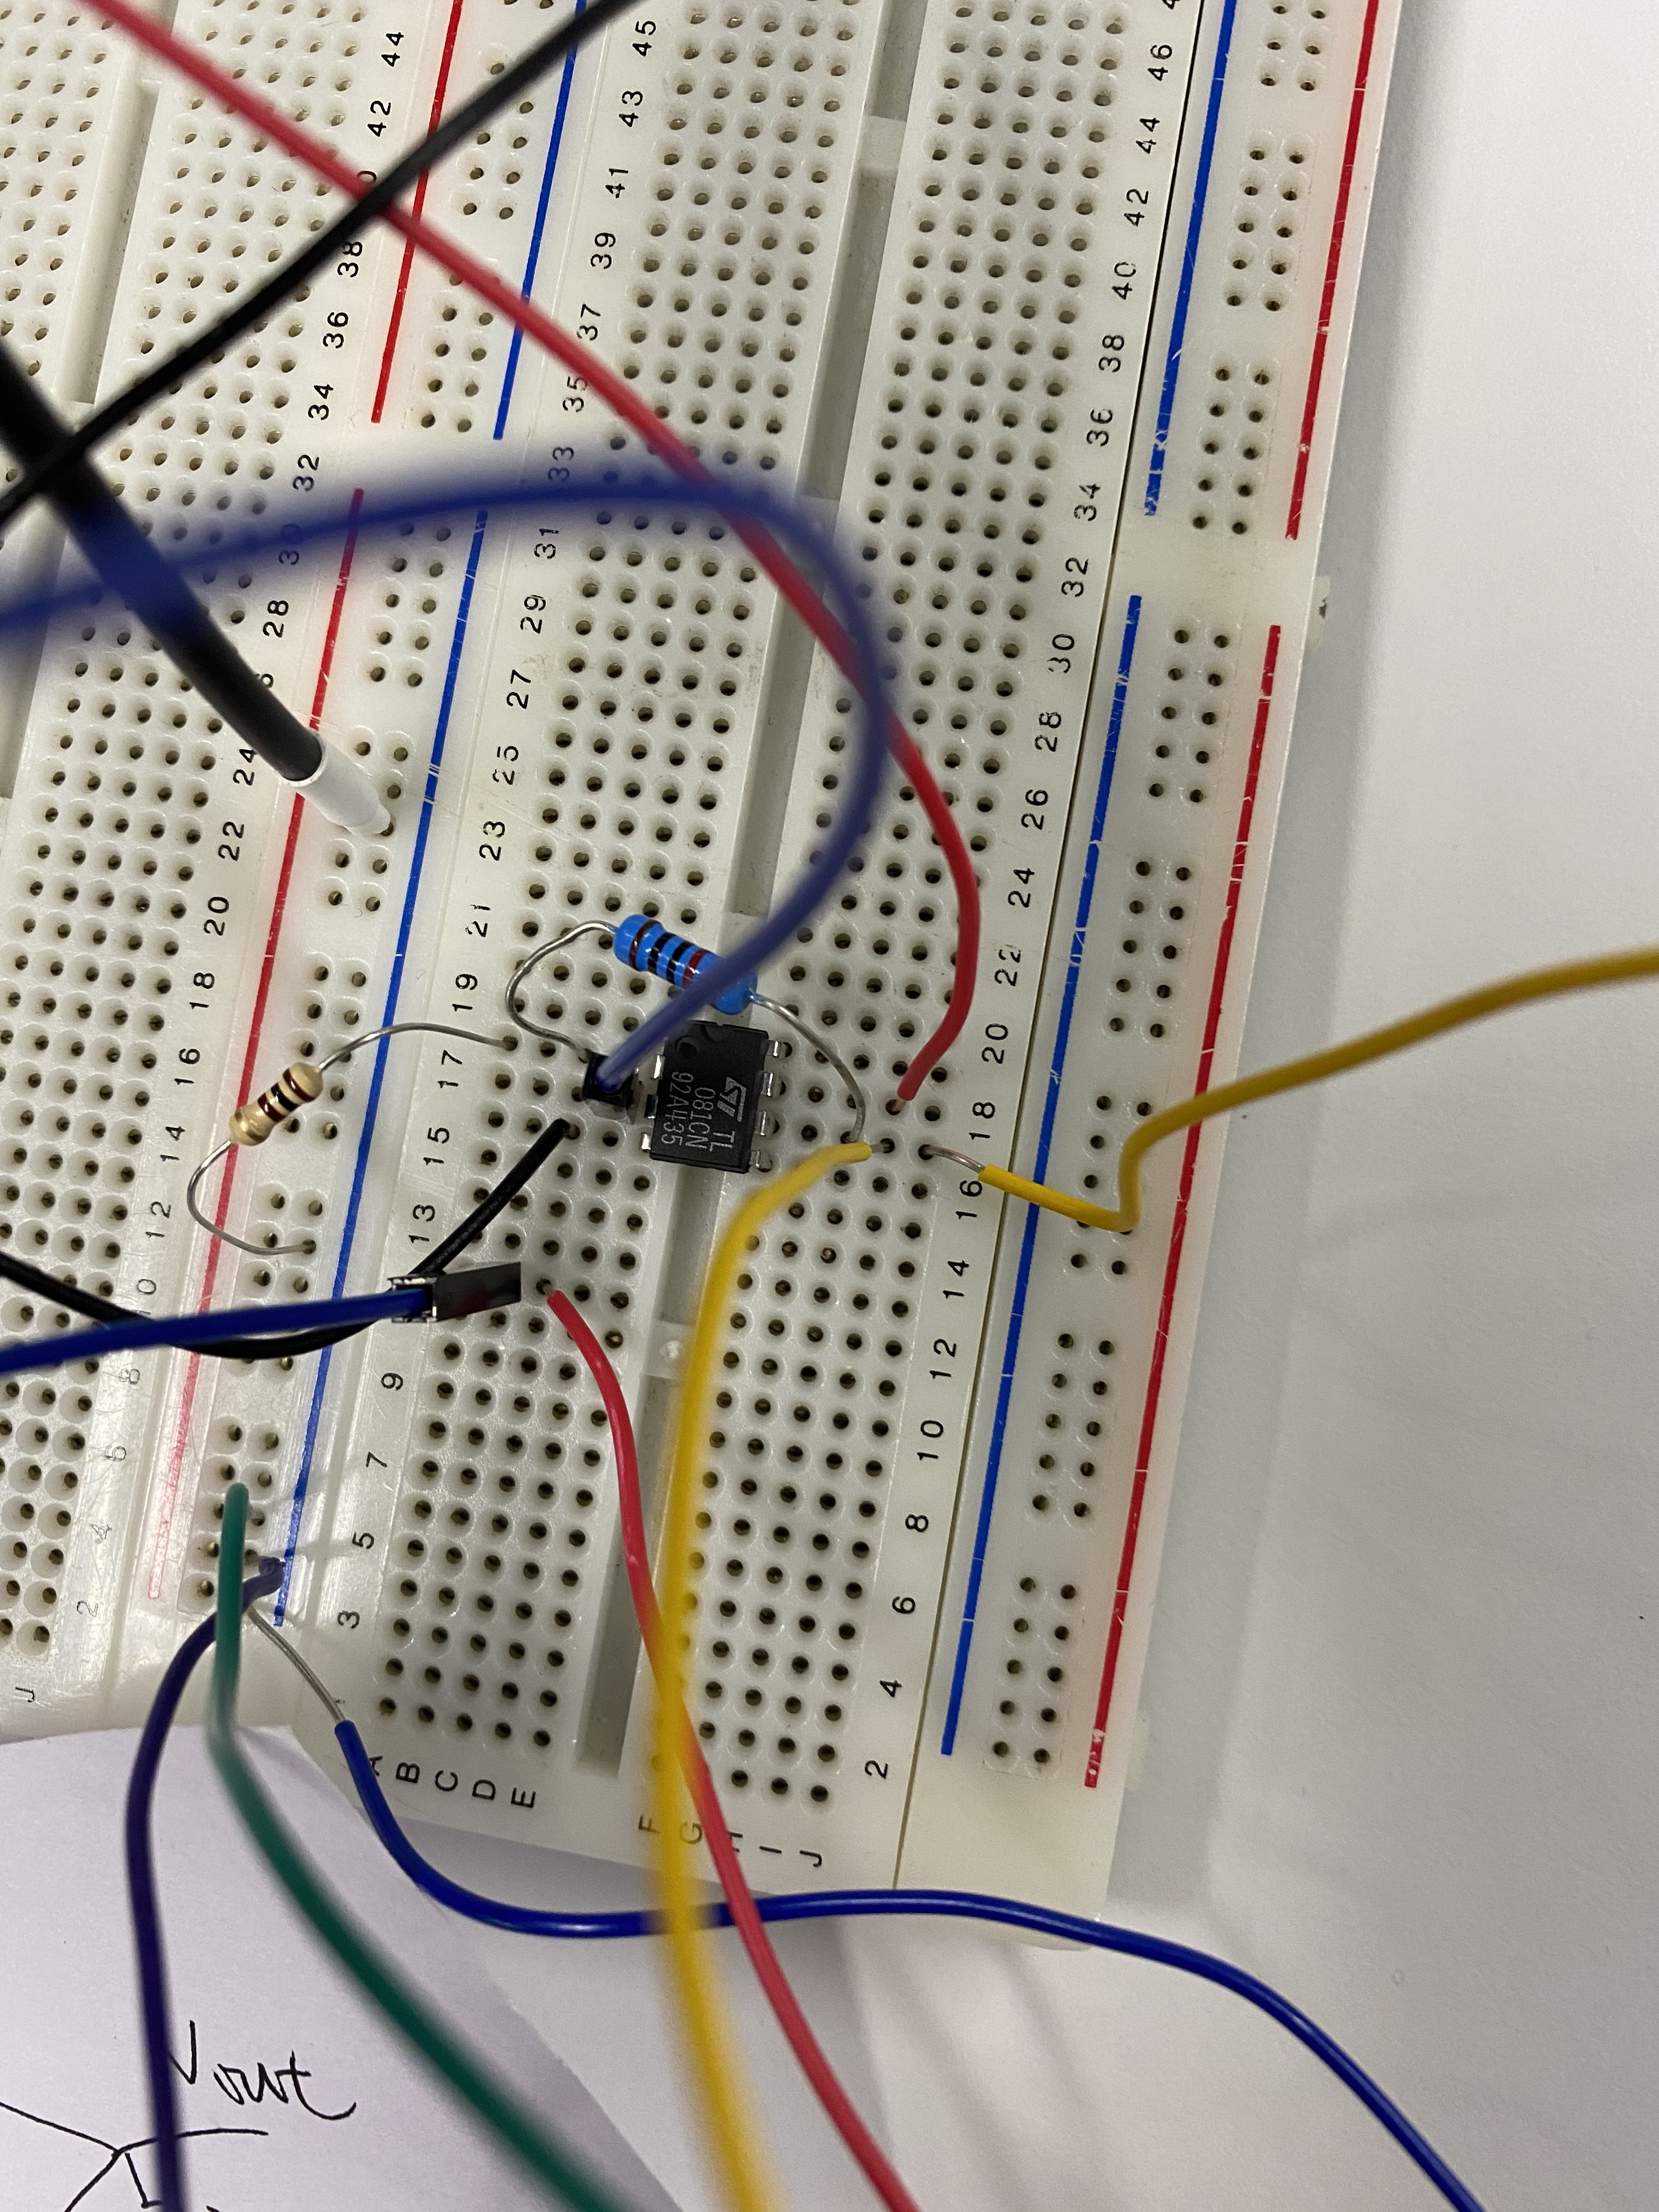
\includegraphics[scale=0.1]{OPAMPAtReceiver.PNG}}
%     \caption{OPAMP at receiver side}
%     \label{fig:OPAMPR}
% \end{figure}
% \begin{figure}
%     \centerline{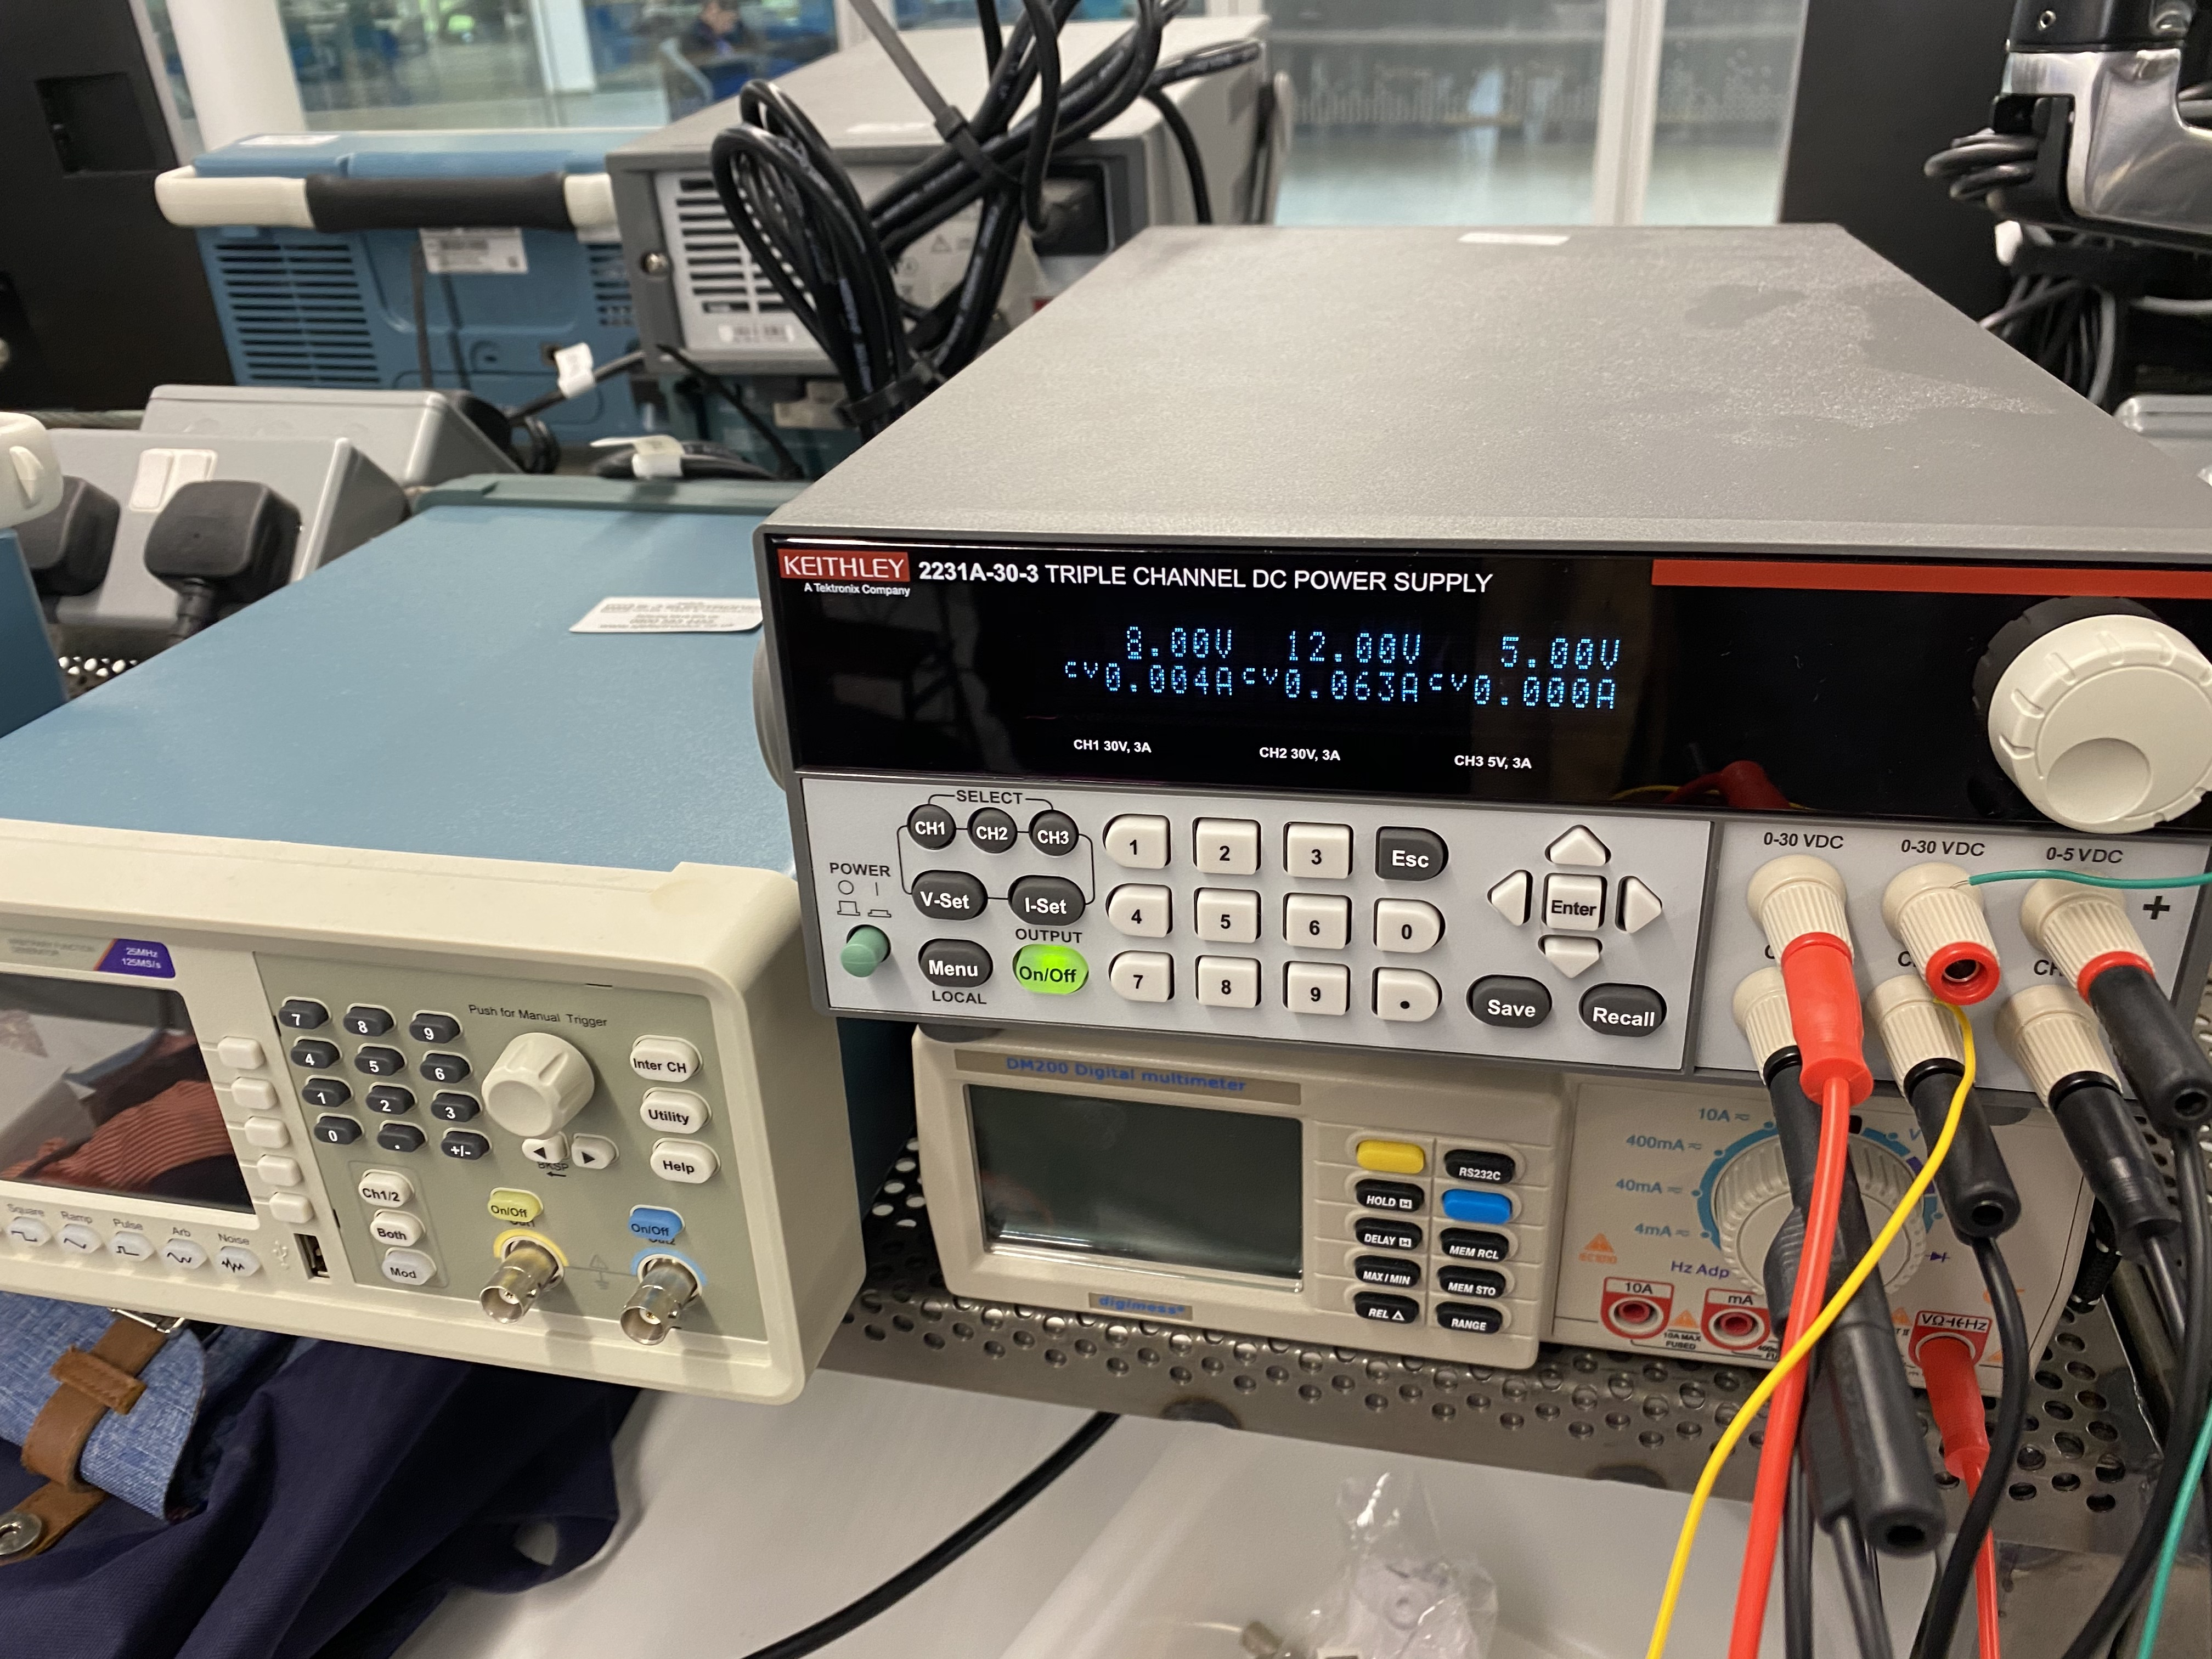
\includegraphics[scale=0.1]{DC_PowerSupplyReceiver.PNG}}
%     \caption{DC power supply at receiver side}
%     \label{fig:DCR}
% \end{figure}

\hyperref[fig:raw_bit_waveform]{Figure \ref*{fig:raw_bit_waveform}} shows the successful example acquired in the laboratory, where the upper one is the signal at the transmitter PC, and the lower one is the signal at the receiver PC.
% \hyperref[fig:DCT]{Figure \ref*{fig:DCT}} to \hyperref[fig:DCR]{Figure \ref*{fig:DCR}} are the components in the wireless communication system. DC power supplies, OPAMPS, oscilators, antennas and low noise amplifier etc. 
\hyperref[fig:DataR]{Figure \ref*{fig:DataR}} shows the received data. the data has been compared to the data at transmitter and no mistake happened.
% \section{Envelope Detector}

\begin{figure}[ht]
    \centerline{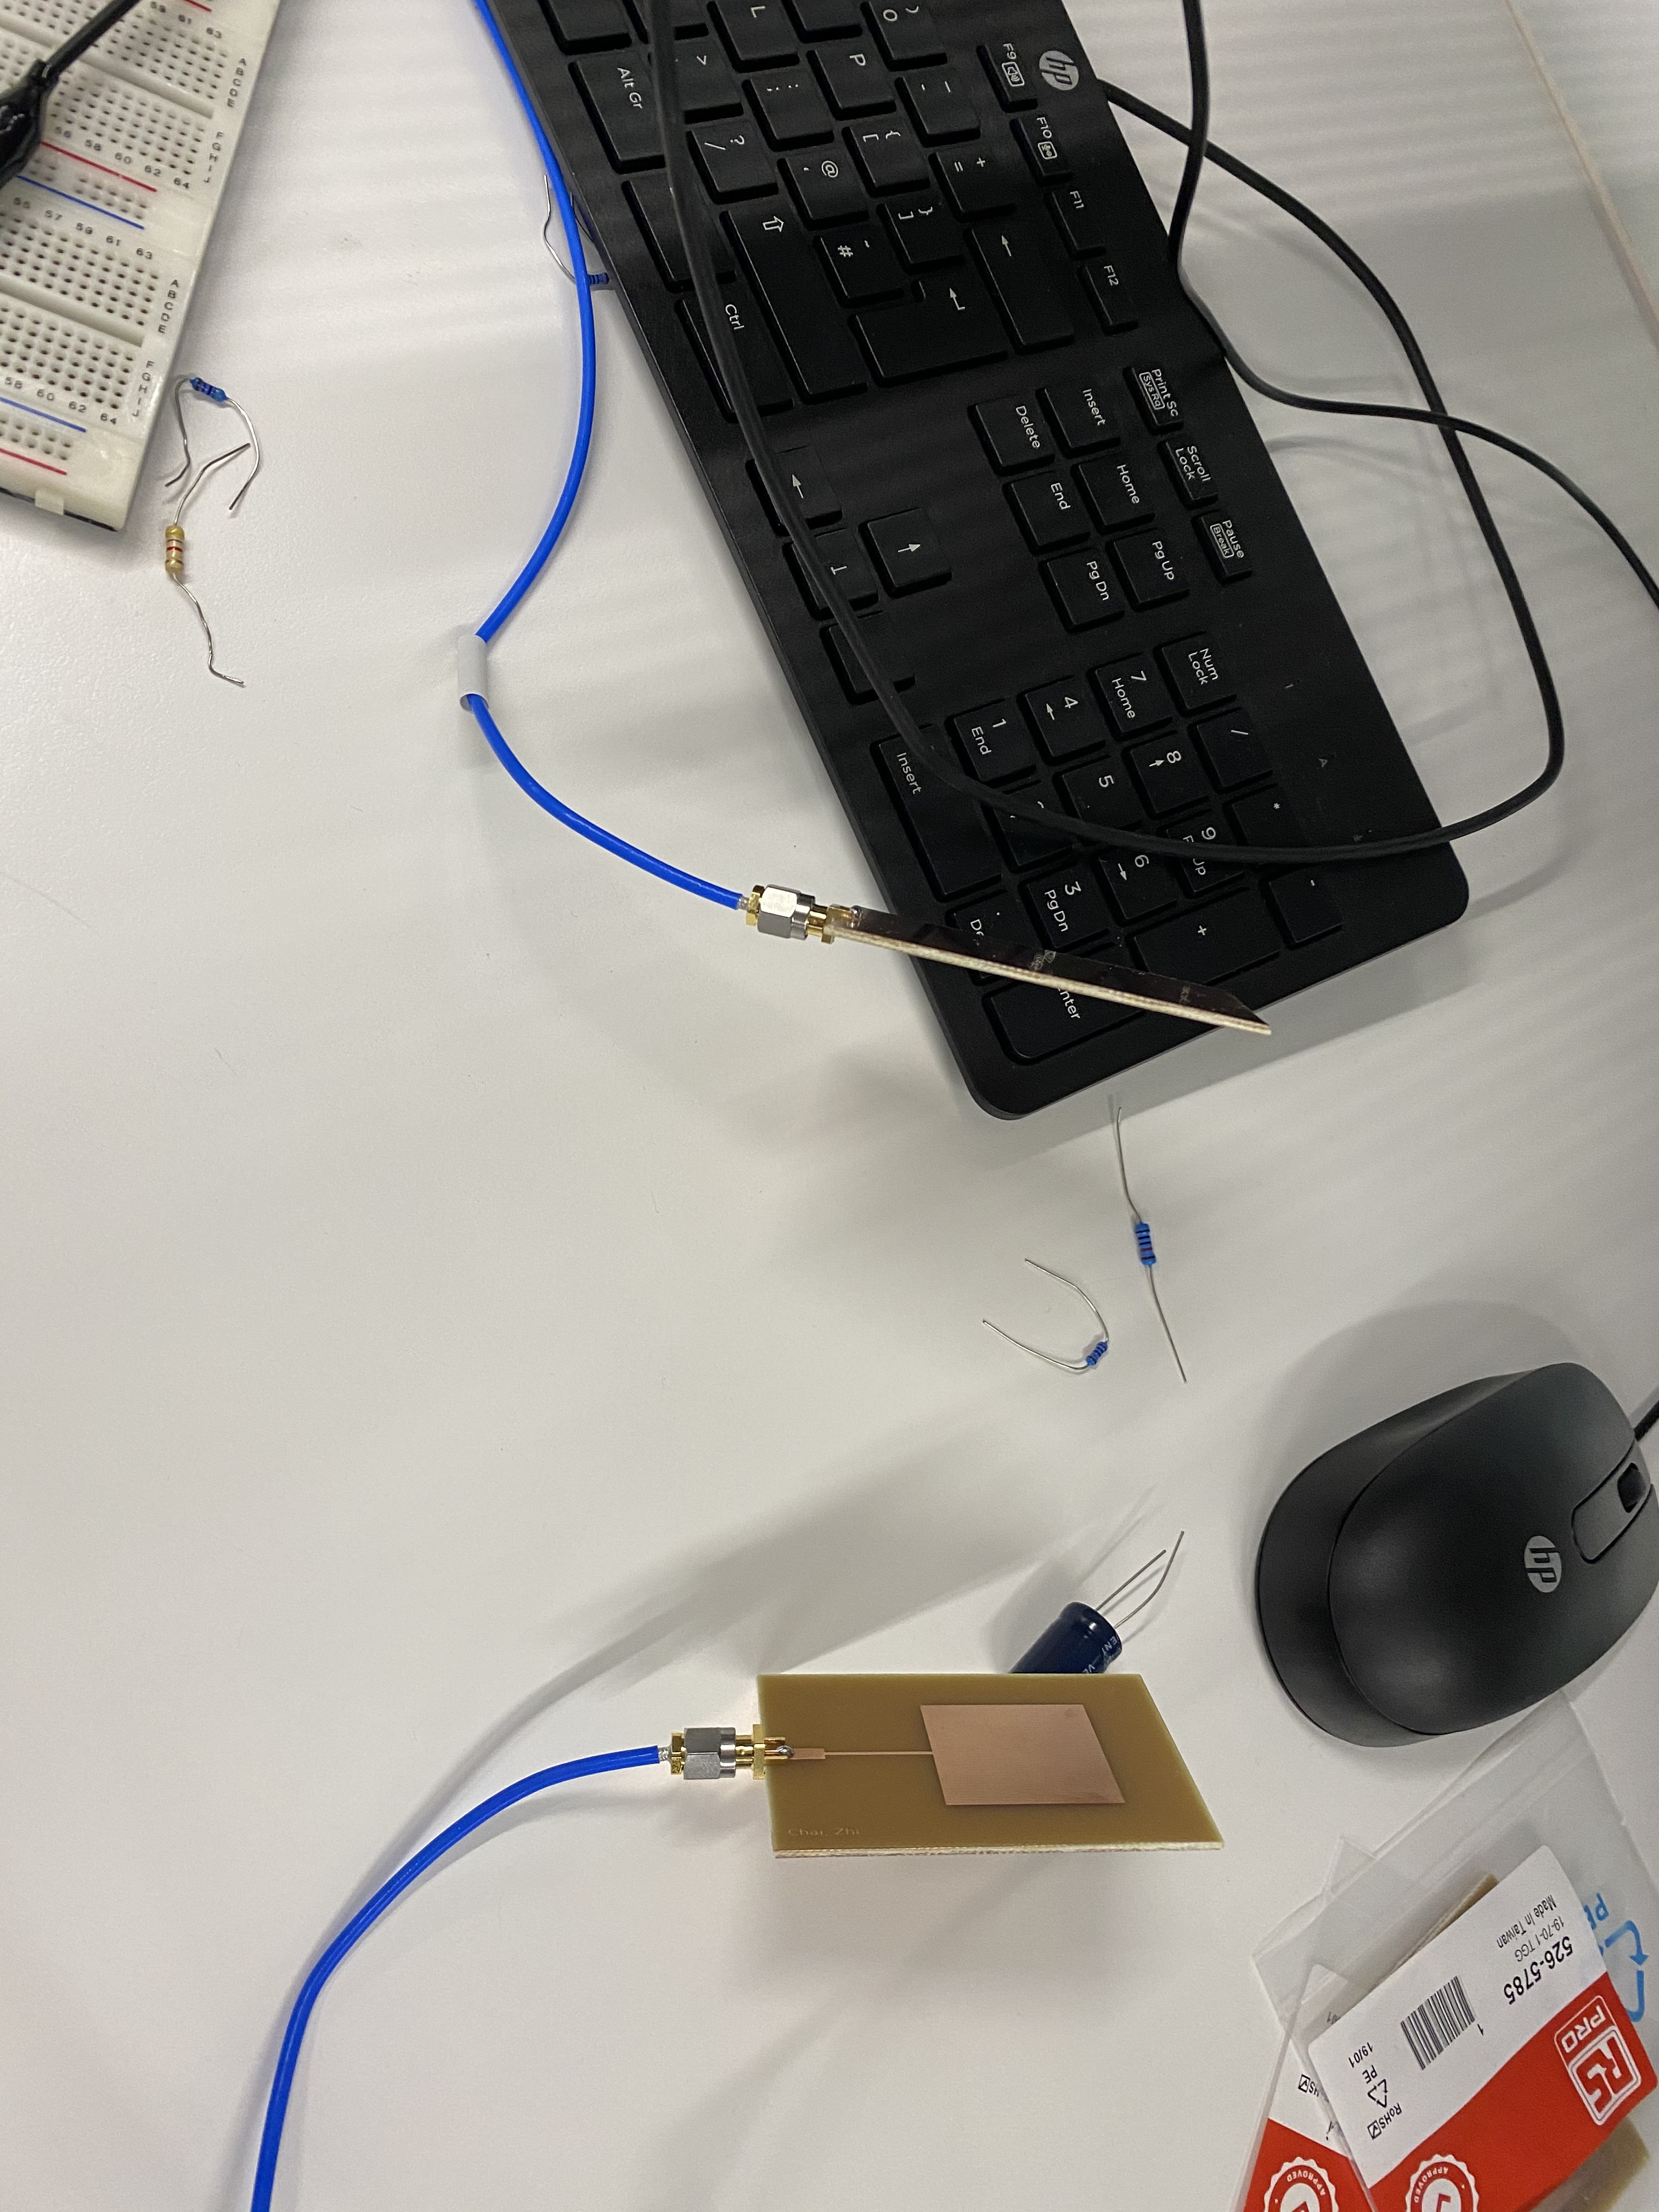
\includegraphics[scale=0.1]{Antennas}}
    \caption{Photo of antennas}
    \label{fig:antennas}
\end{figure}

\begin{figure}[htp]
    \begin{center}
      \subfigure[The test of LPF under 1KHz]
      {\label{fig:LPF_1KHz}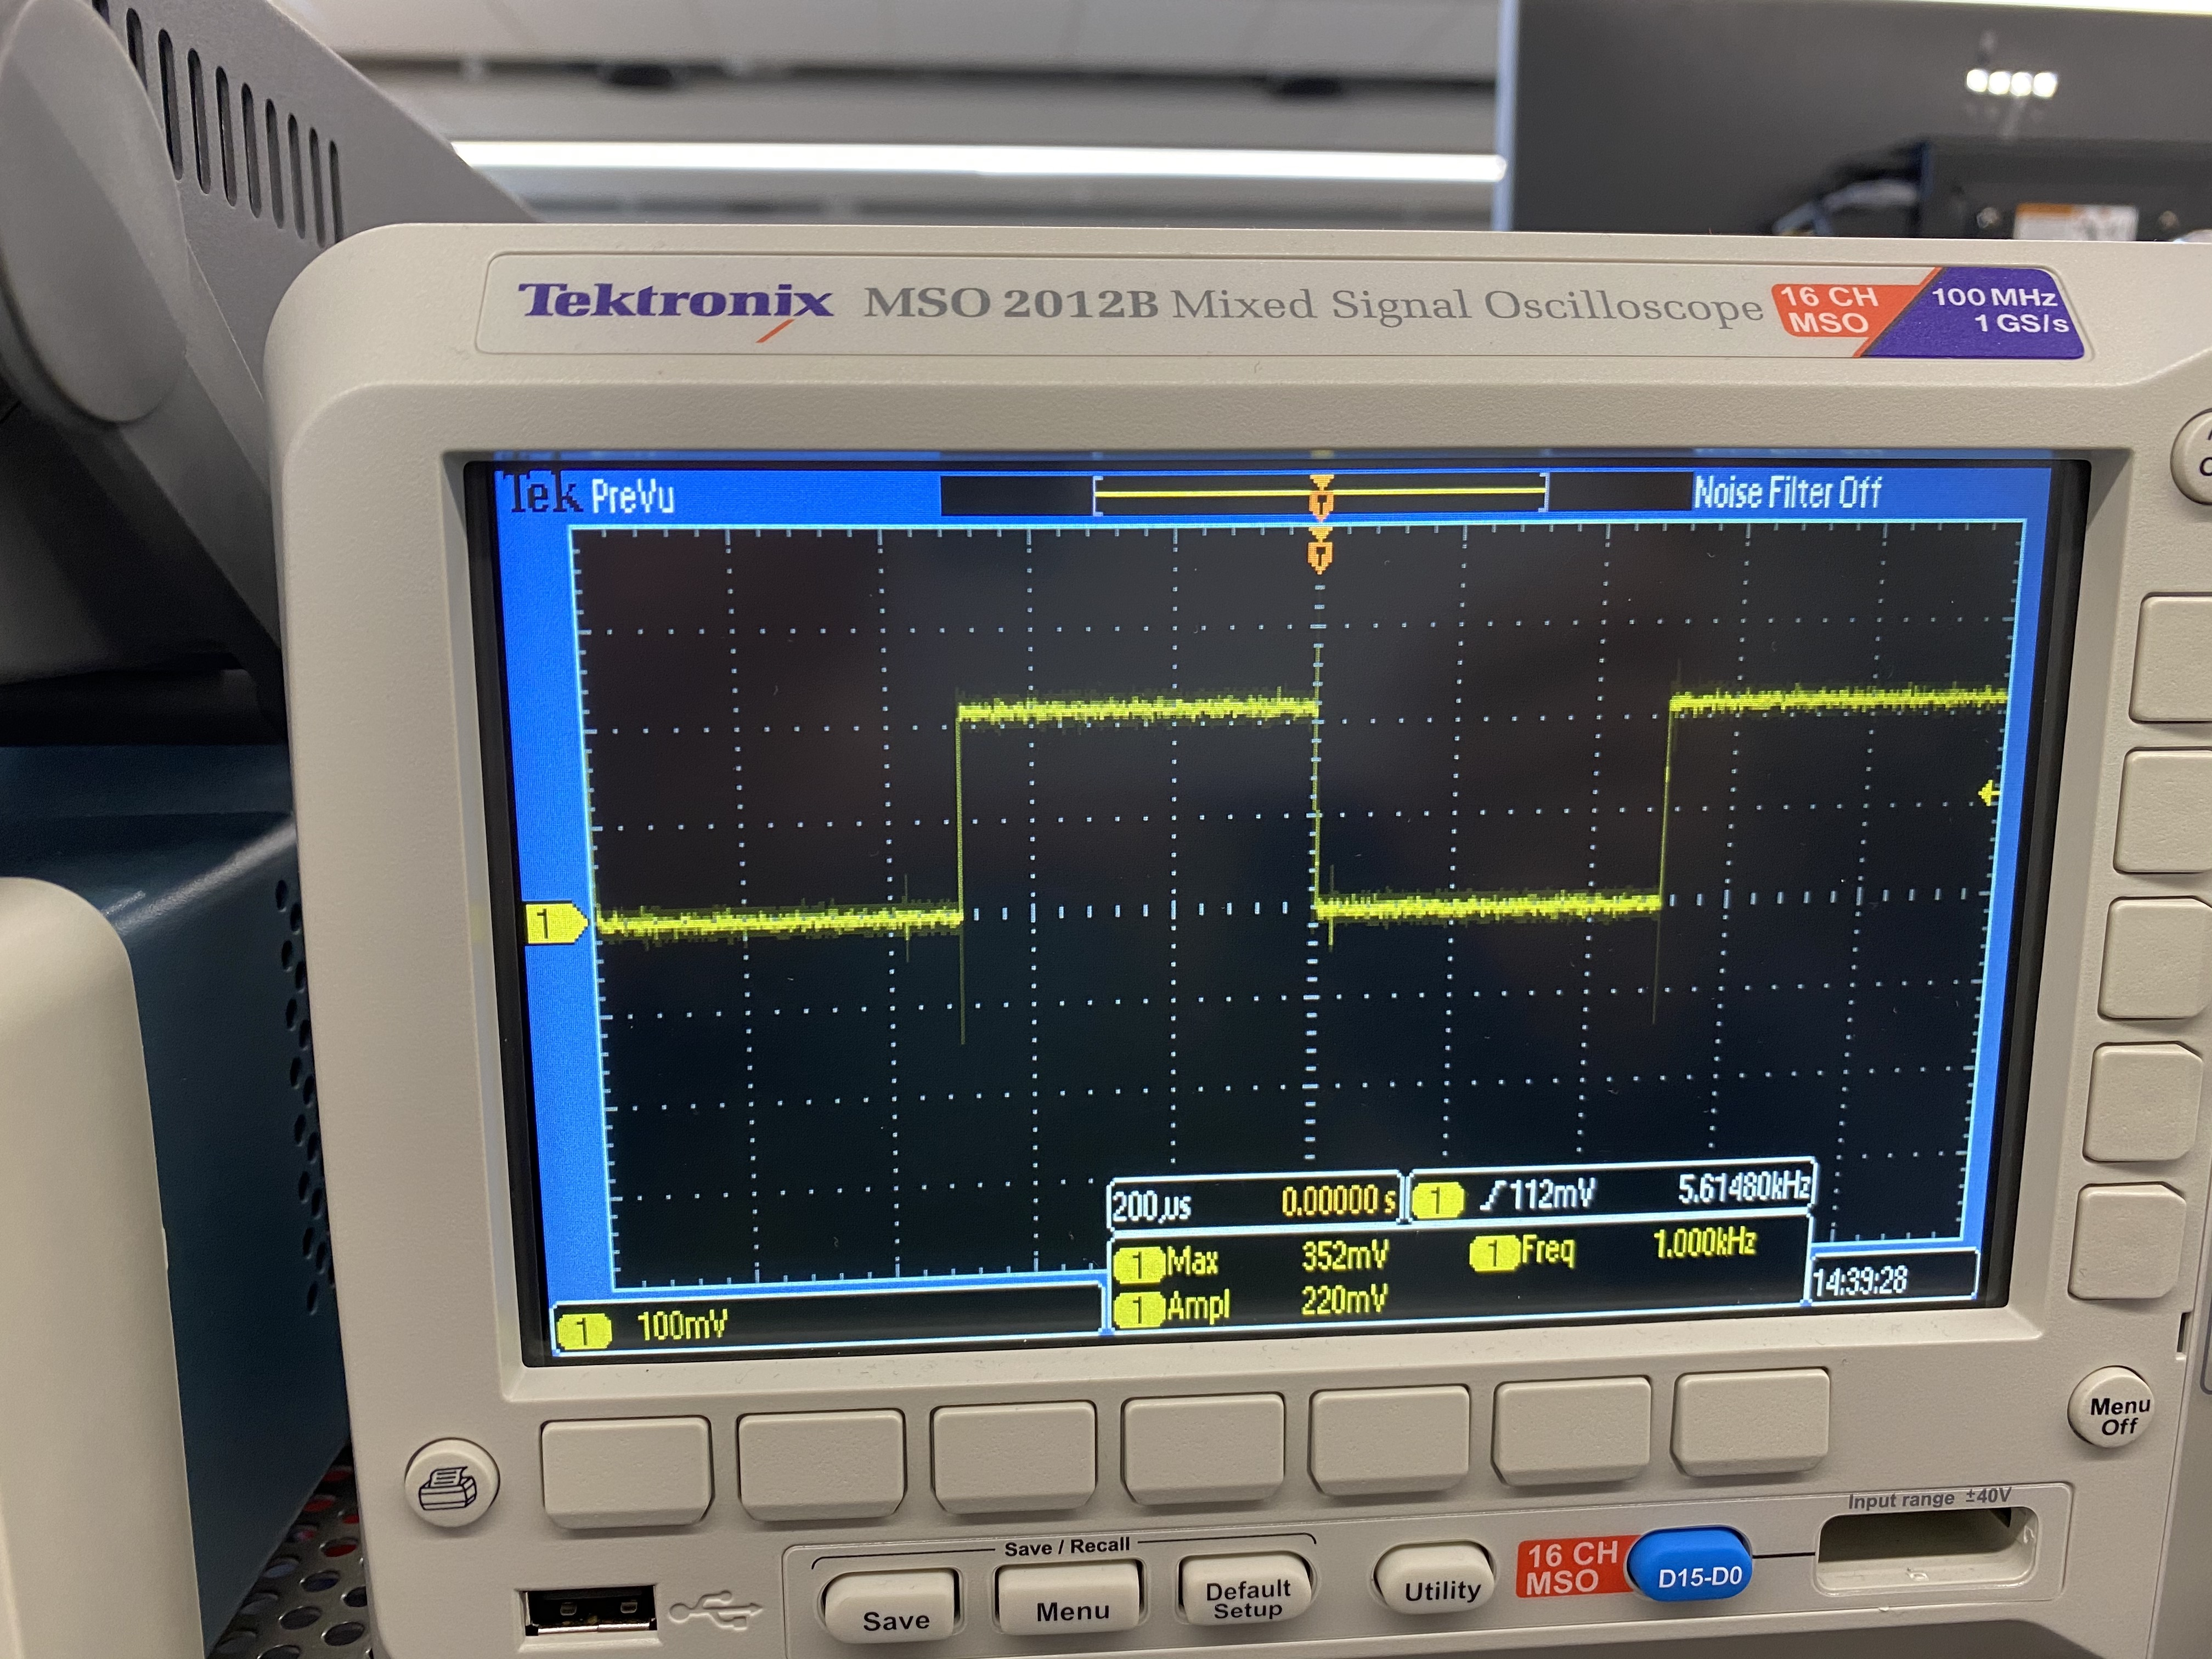
\includegraphics[width=.49\linewidth]{LPFTest1KHz}}
      \subfigure[The test of LPF under 2Hz]
      {\label{fig:LPF_2Hz}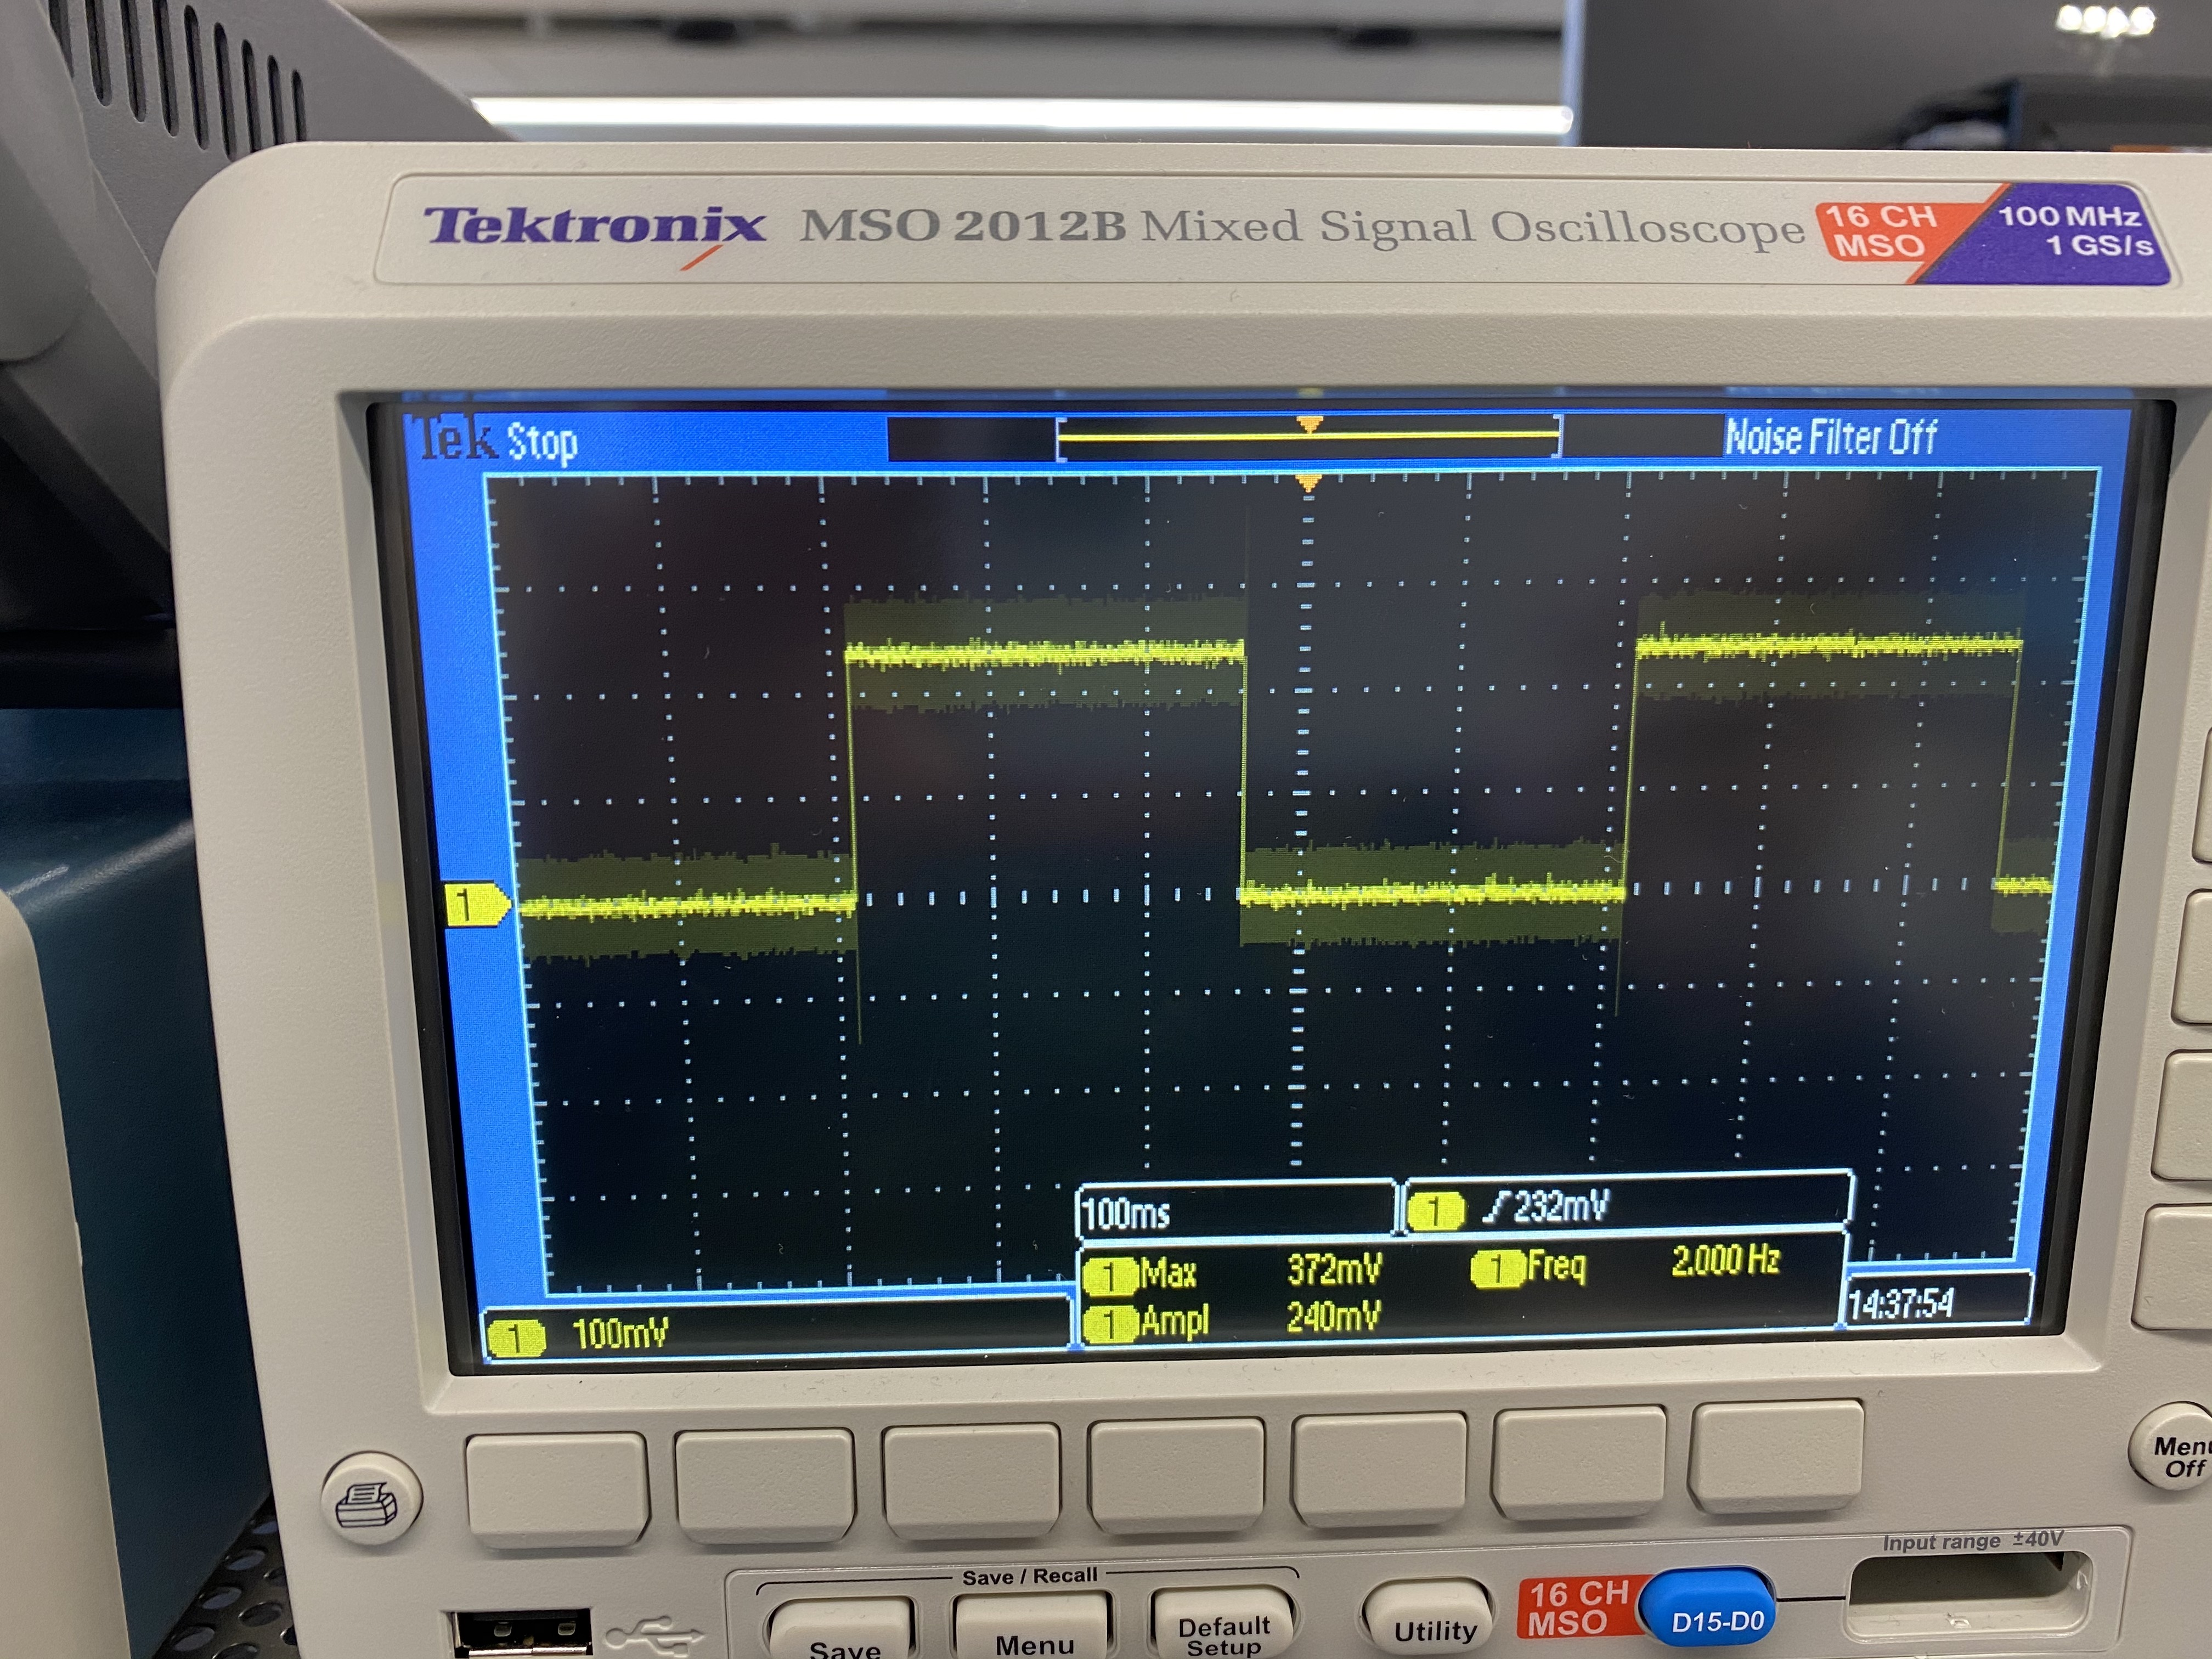
\includegraphics[width=.49\linewidth]{LPFTest2Hz}} \\
      \subfigure[The test of LPF under 5Hz]
      {\label{fig:LPF_5Hz}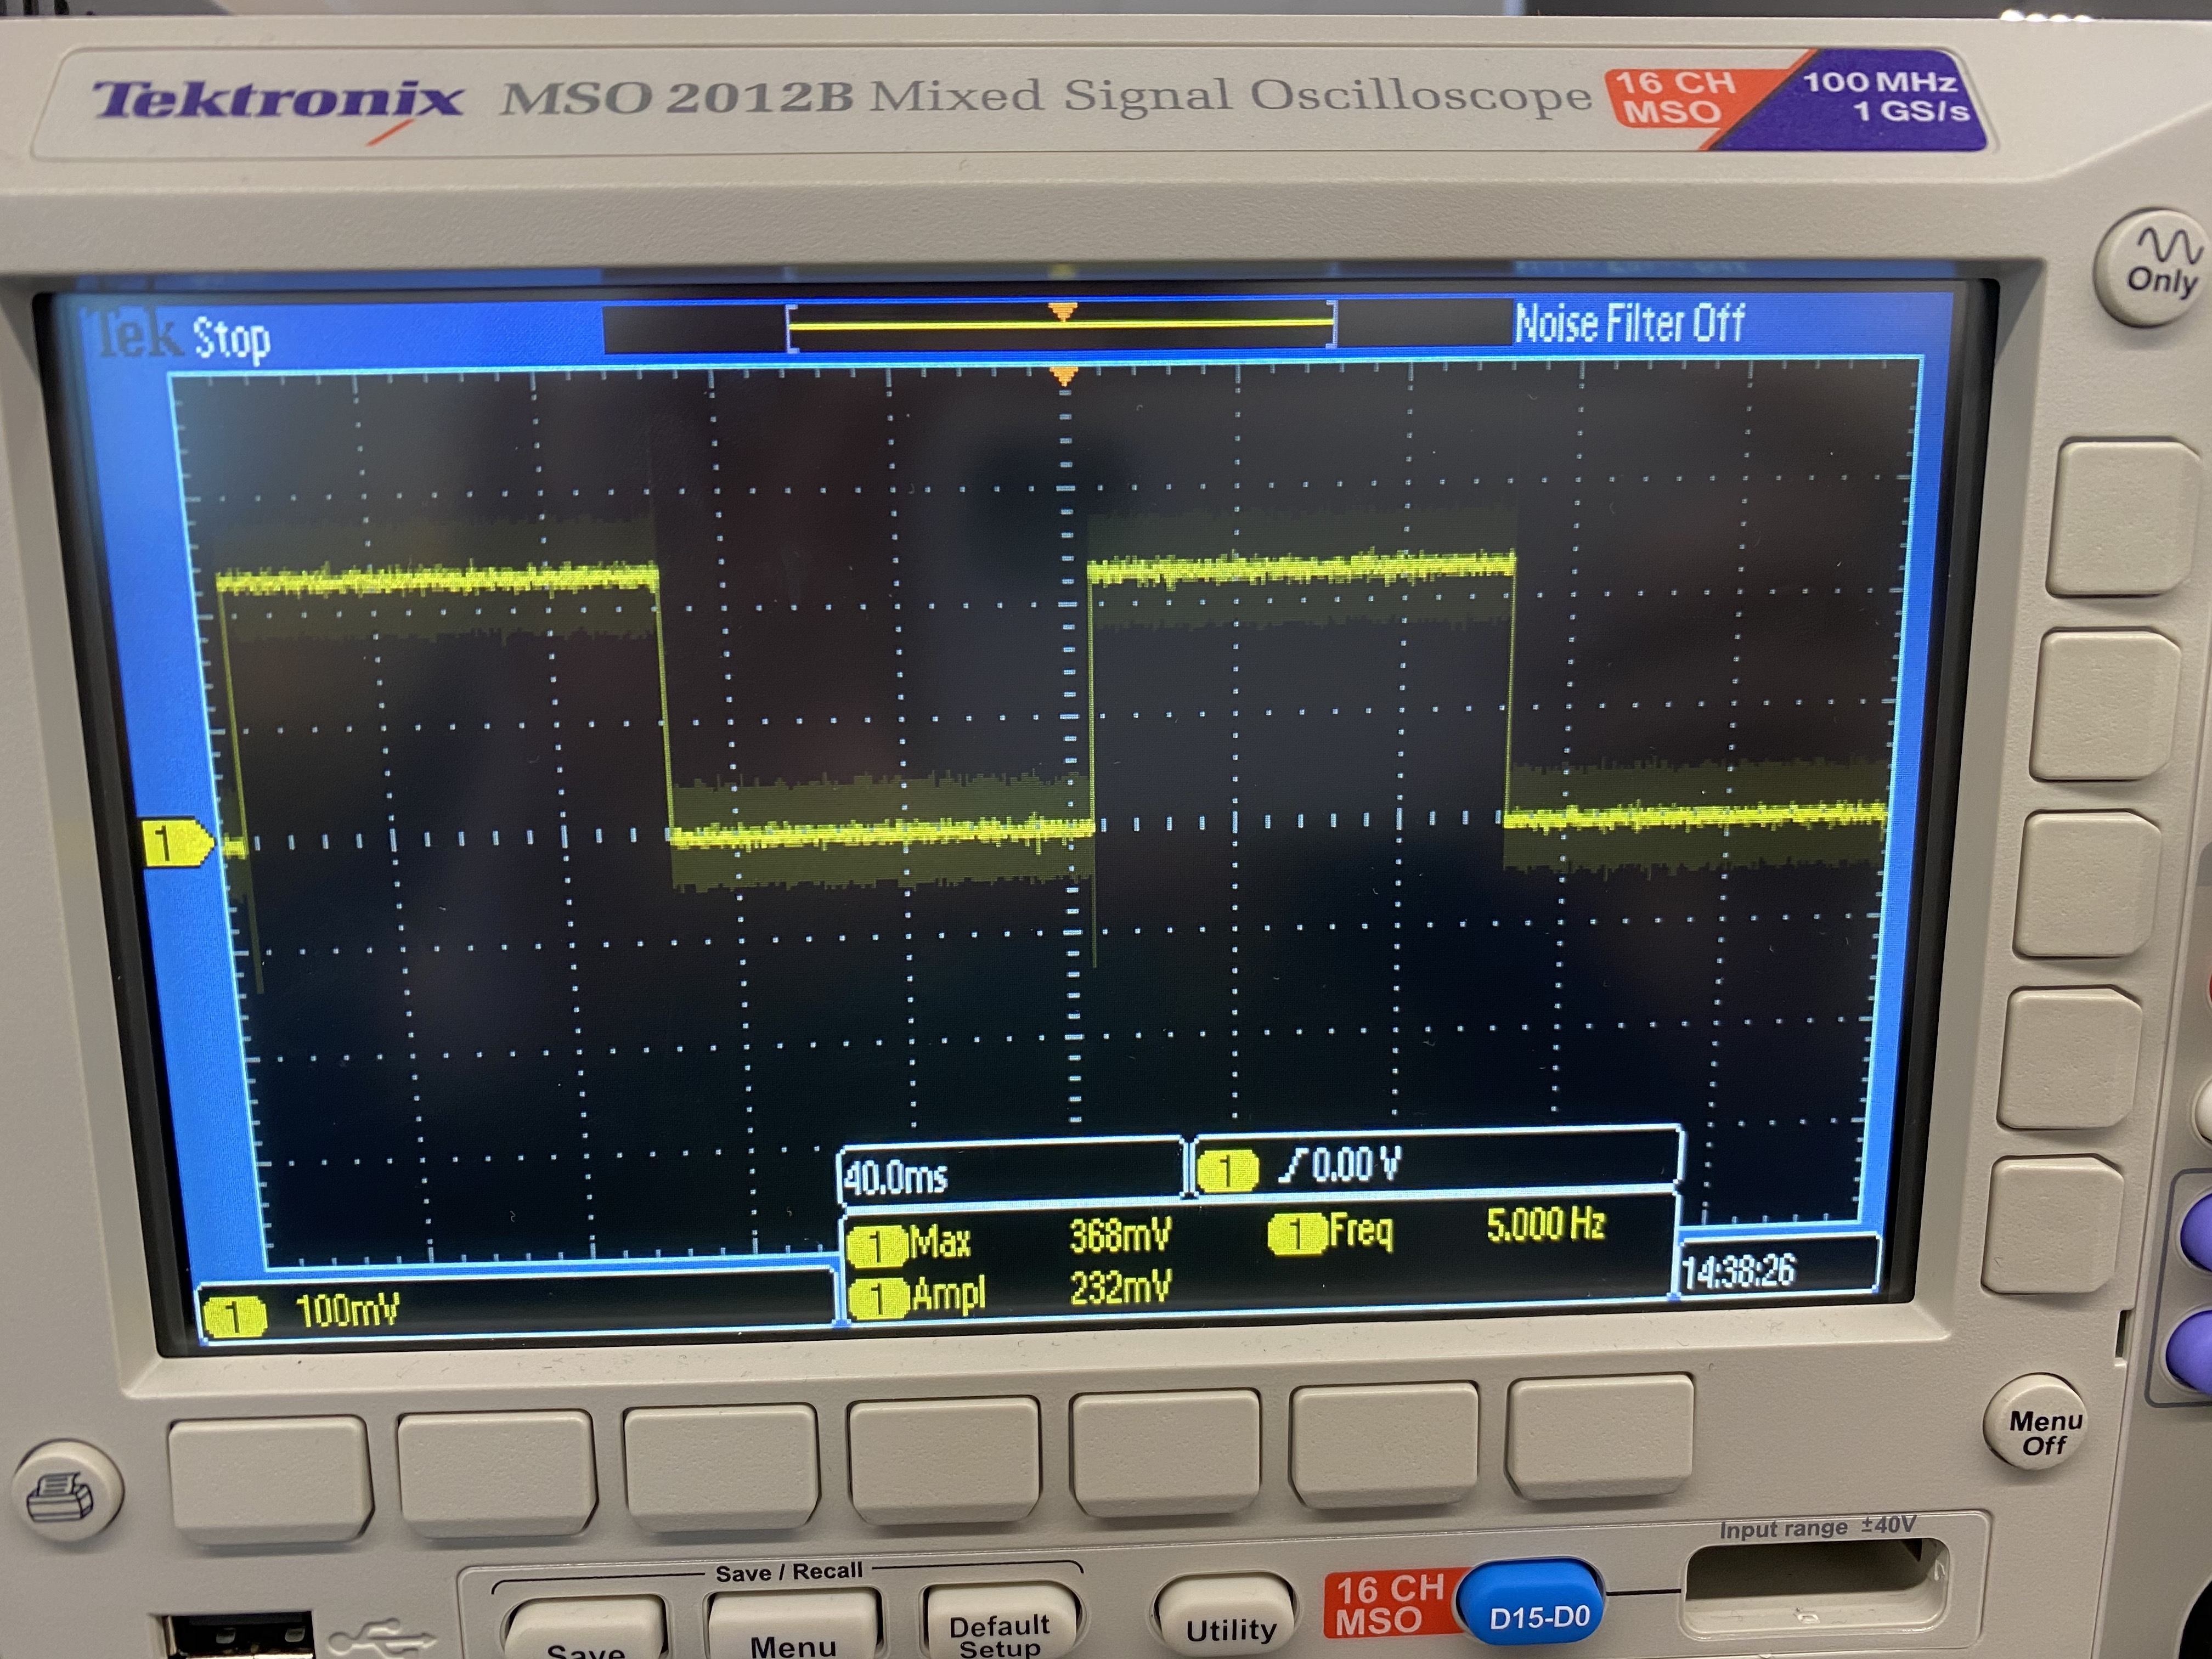
\includegraphics[width=.5\linewidth]{LPFTest5Hz}}
    \end{center}
    \caption{The performance of test of LPF}
    \label{fig:LPF_test}
\end{figure}

\begin{figure}[htp]
    \begin{center}
        \subfigure[transmittor op-amp]
        {\label{fig:trans_op_amp}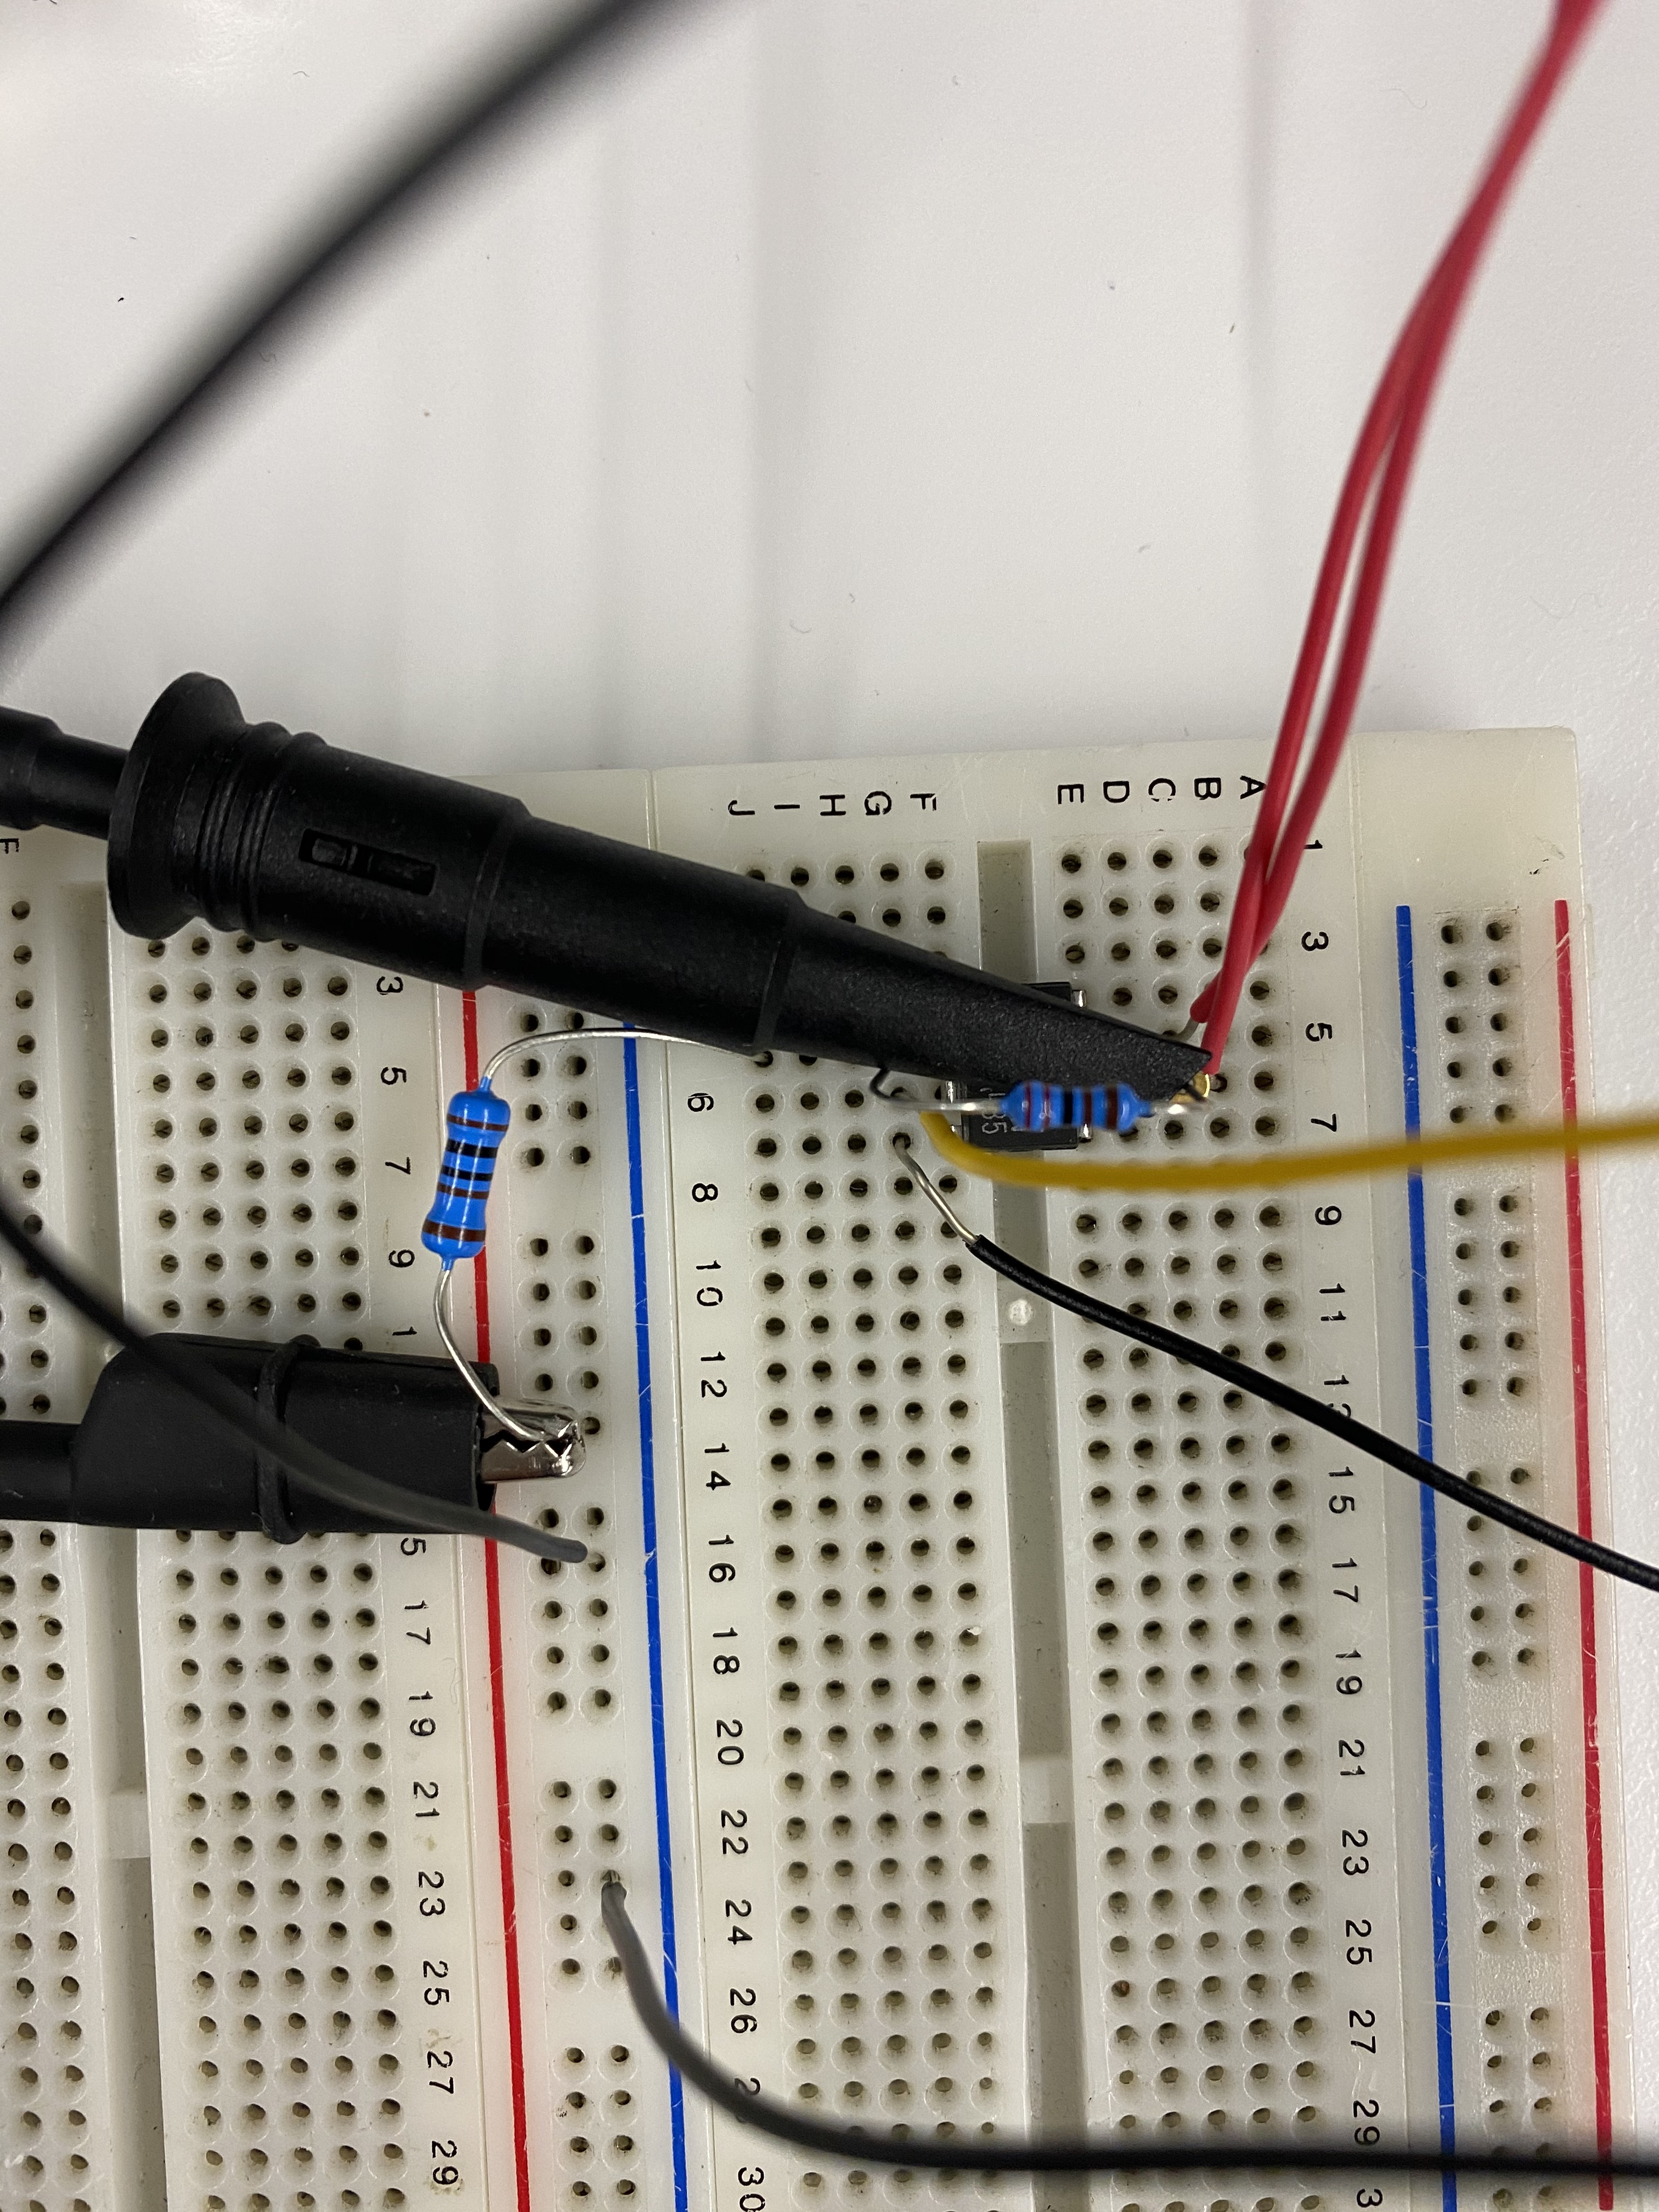
\includegraphics[width=.48\linewidth]{OPAMP_Transmitter}}
        \subfigure[receiver op-amp]
        {\label{fig:recev_op_amp}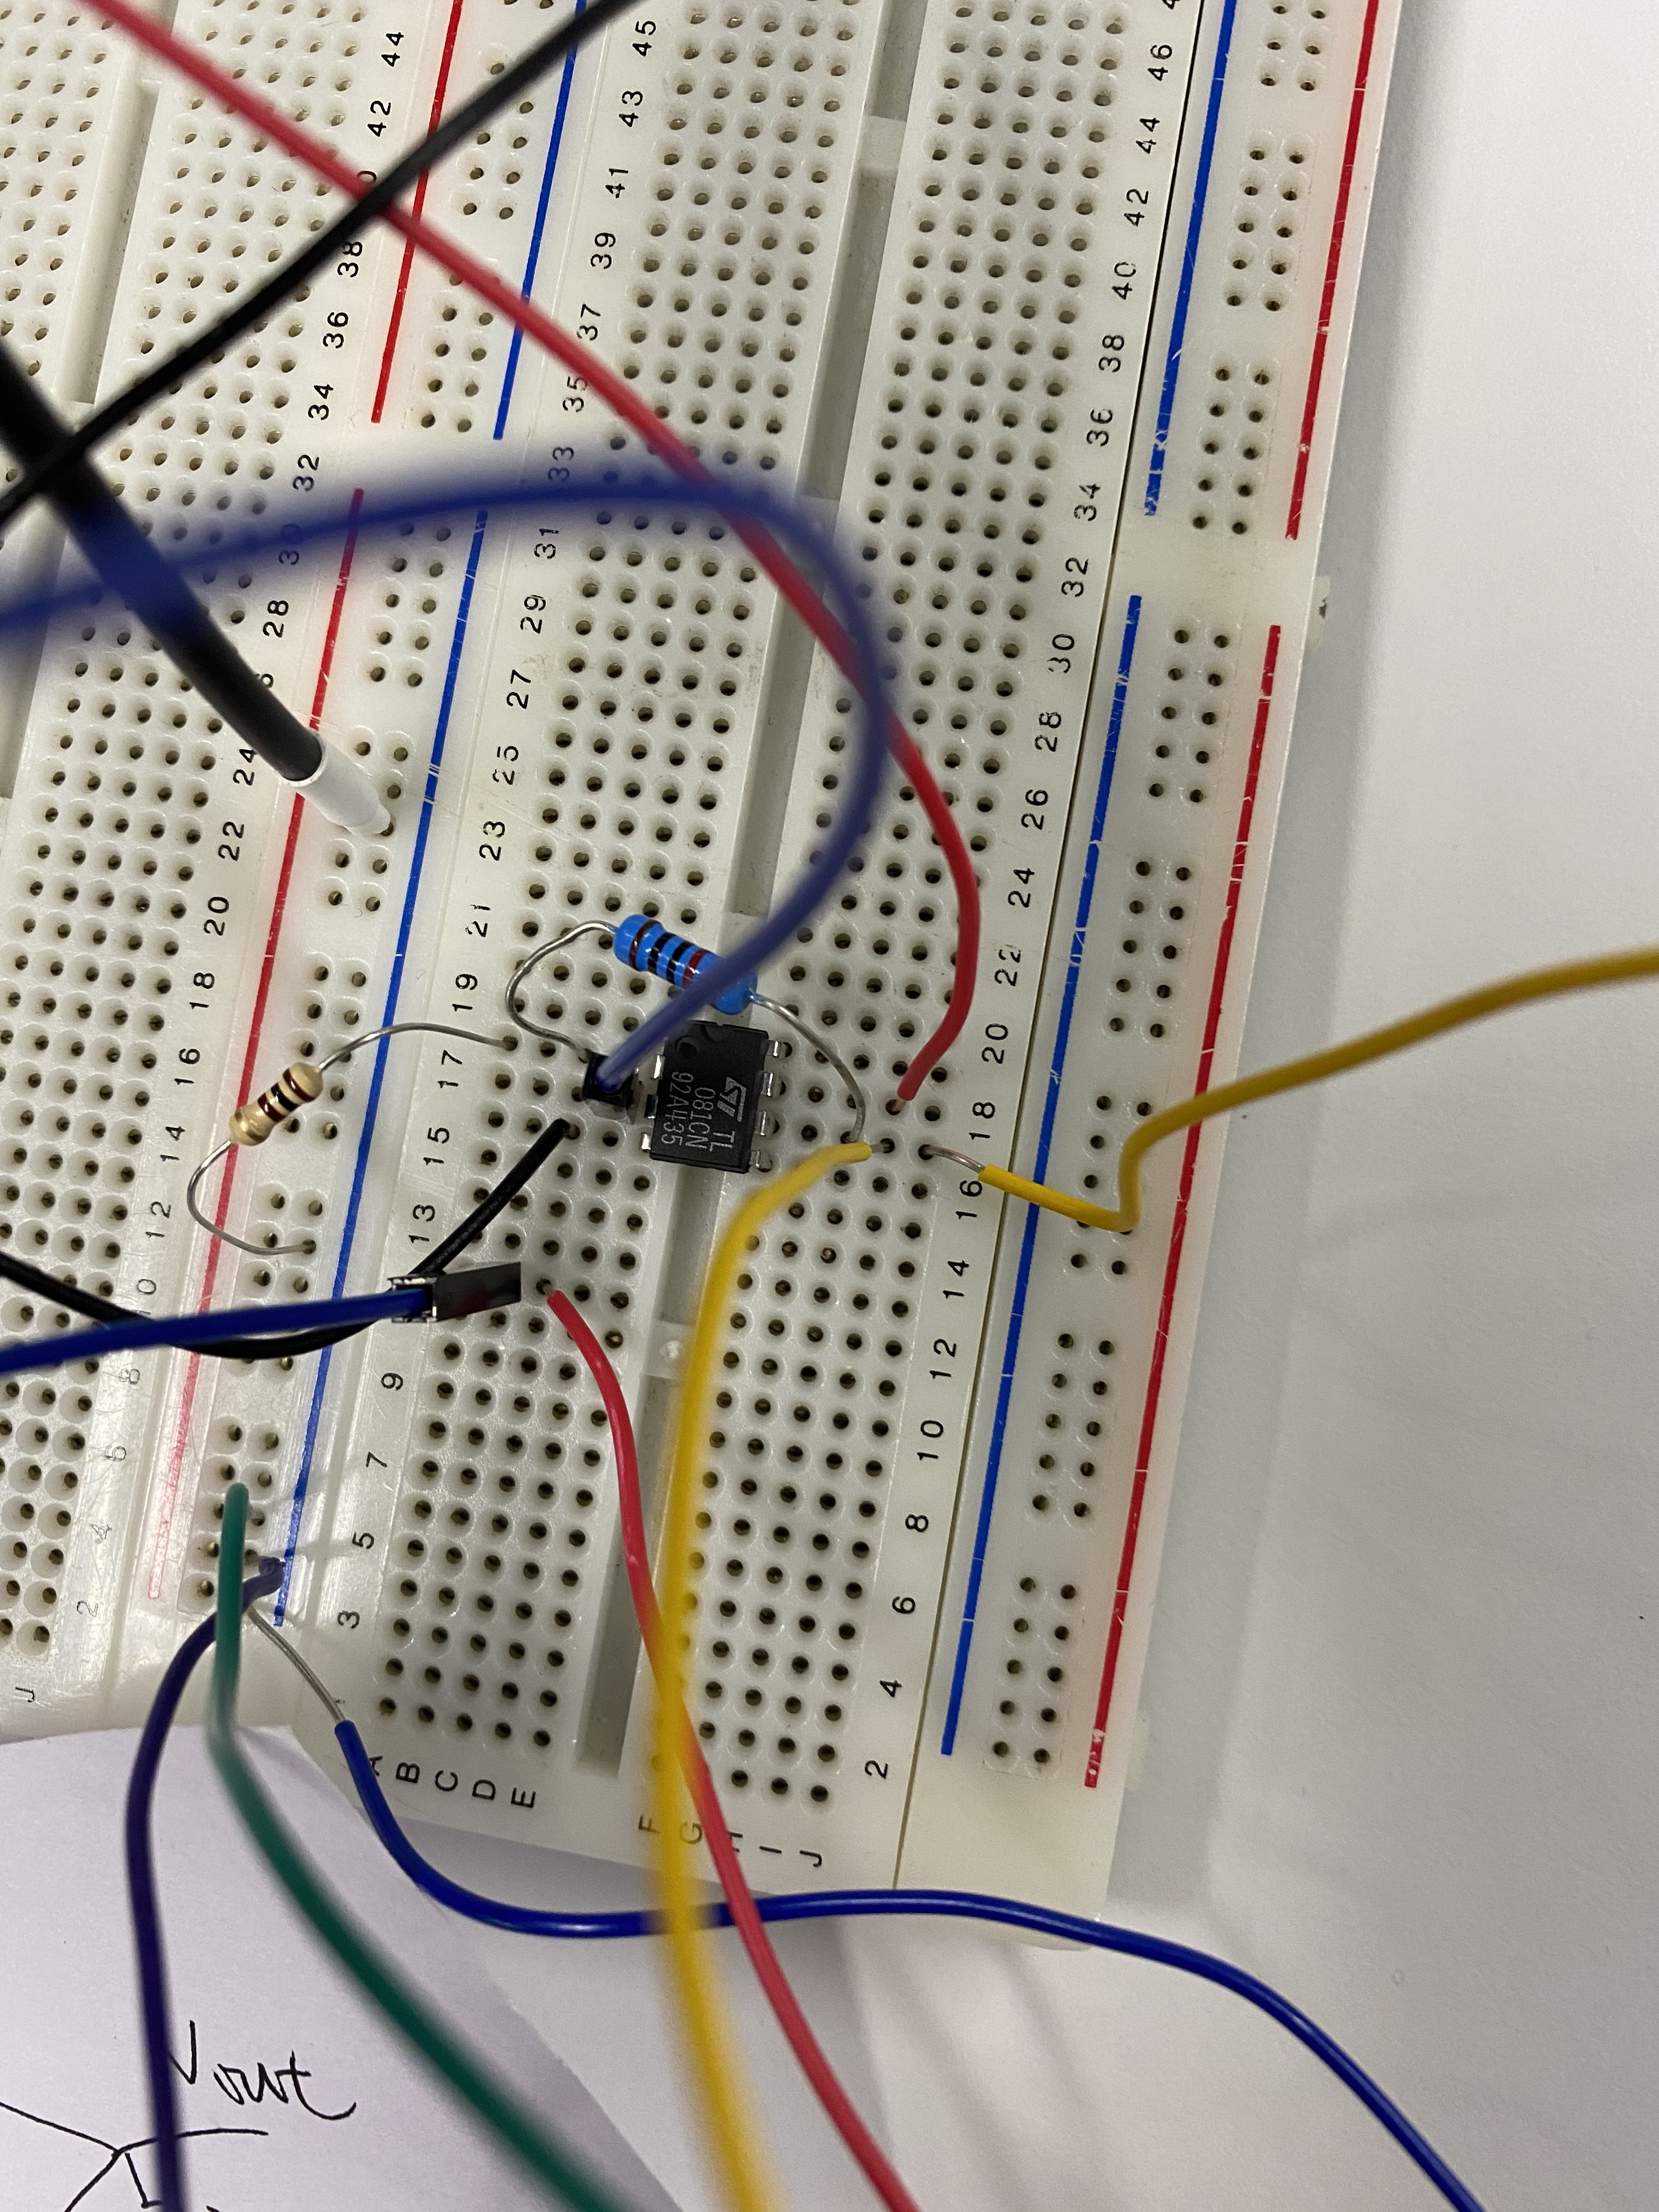
\includegraphics[width=.48\linewidth]{OPAMPAtReceiver}}
    \end{center}
    \caption{Photos of op-amps}
    \label{fig:opamps}
\end{figure}

\begin{figure}
    \centerline{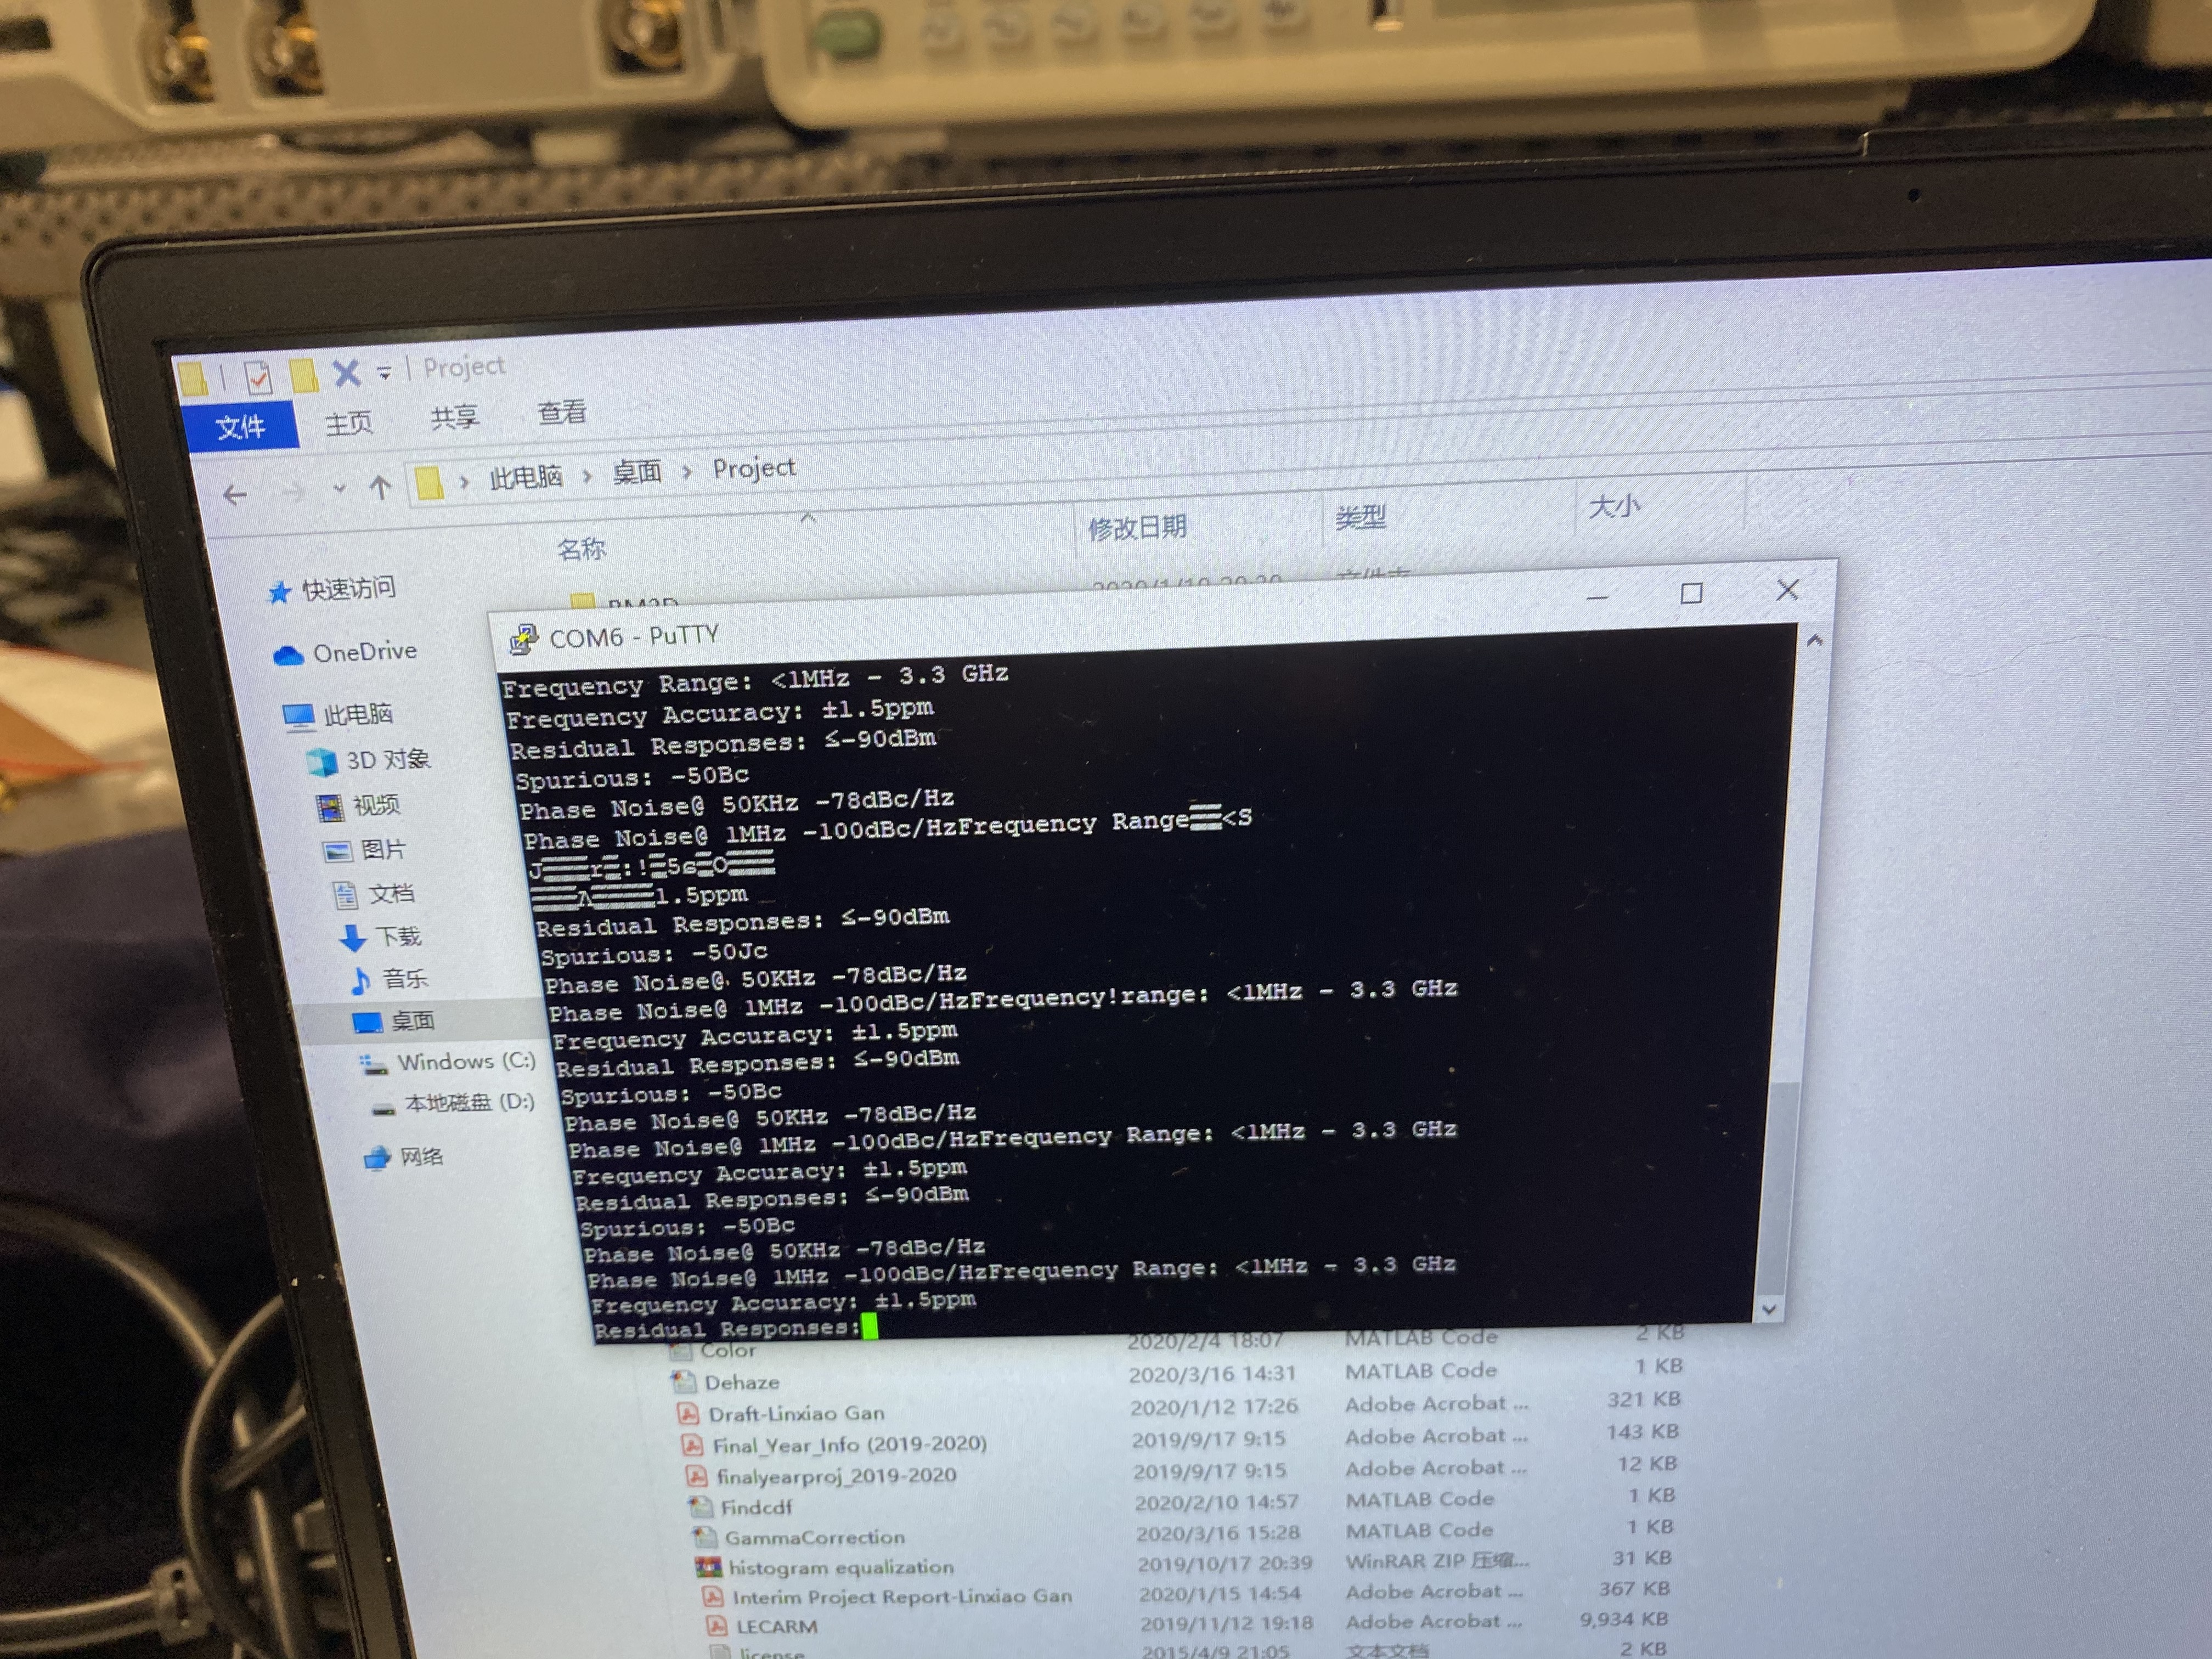
\includegraphics[scale=0.1]{ReceiverPC.png}}
    \caption{Received data}
    \label{fig:DataR}
\end{figure}

\begin{thebibliography}{99}

    \bibitem{input_impedance}
    J.D. Kraus , R.J. Marhafka.
    \textit{Antennas for All Applications, $3^{rd}$ ed.}
    Boston MA: McGraw Hill, 2002, p. 324.


\end{thebibliography}
    
\end{document}